%!TeX root = main.tex
%!TeX root = 2-thermo.tex
\documentclass[main.tex]{subfiles}

\begin{document}

\chapter{Thermodynamic Exploration of Xenon/Krypton Separation}
\vspace*{-1\baselineskip}

\section{Characterization of adsorption equilibrium properties}

Before exploring the thermodynamic properties of the adsorption-based xenon/krypton separation, this first section aims at  defining some key concepts that will be referenced throughout this manuscript. These concepts include the computational definition of the geometrical descriptors mentioned in Chapter 1, as well as the molecular simulations used to assess the separation performance of each material. In addition, the definition of these thermodynamic quantities will be elucidated to ensure a better understanding of the work presented in the following sections.

\subsection{Geometrical descriptors}

Before delving into the details of adsorption properties, it is important to introduce the different simulation techniques used to characterize the internal pore structure of the material. These properties play an essential role in interpreting the adsorption properties obtained using more complex molecular simulations. In this thesis, the Zeo++ software was utilized to calculate all the geometrical descriptors used.\autocite{Zeo++} While other tools exist,\autocite{First_2013,PoreBlazer} the use of Voronoi decomposition of the volume offers computational efficiency advantages (efficiency gain mainly on volume calculation),\autocite{Rycroft_2009} making Zeo++ the preferred tool in this study.

\subsubsection{Pore size}

Different definitions of pore sizes can be defined depending on the point where we measure it. These diverse pore sizes collectively form what is known as a pore size distribution. However, some pore size values are uniquely defined and can be used to characterize the internal structure. For instance, the diameter of the largest sphere that can freely diffuse in the structure is referred to as D$_f$. The diameter D$_{if}$ corresponds to the diameter of the largest included sphere along a free diffusion path. The diameter of the largest included sphere (not necessarily in a free diffusion path) is denoted D$_i$. The Figure~\ref{fgr:pore_size} illustrates the difference between these pore sizes. In thermodynamic studies, the term ``largest cavity diameter'' (LCD) will be frequently employed instead of the largest included sphere D$_i$. Moreover, the term ``pore limiting diameter'' will be used instead of D$_f$, especially when studying the transport effects within the nanopores.

\begin{figure}[ht]
  \centering
  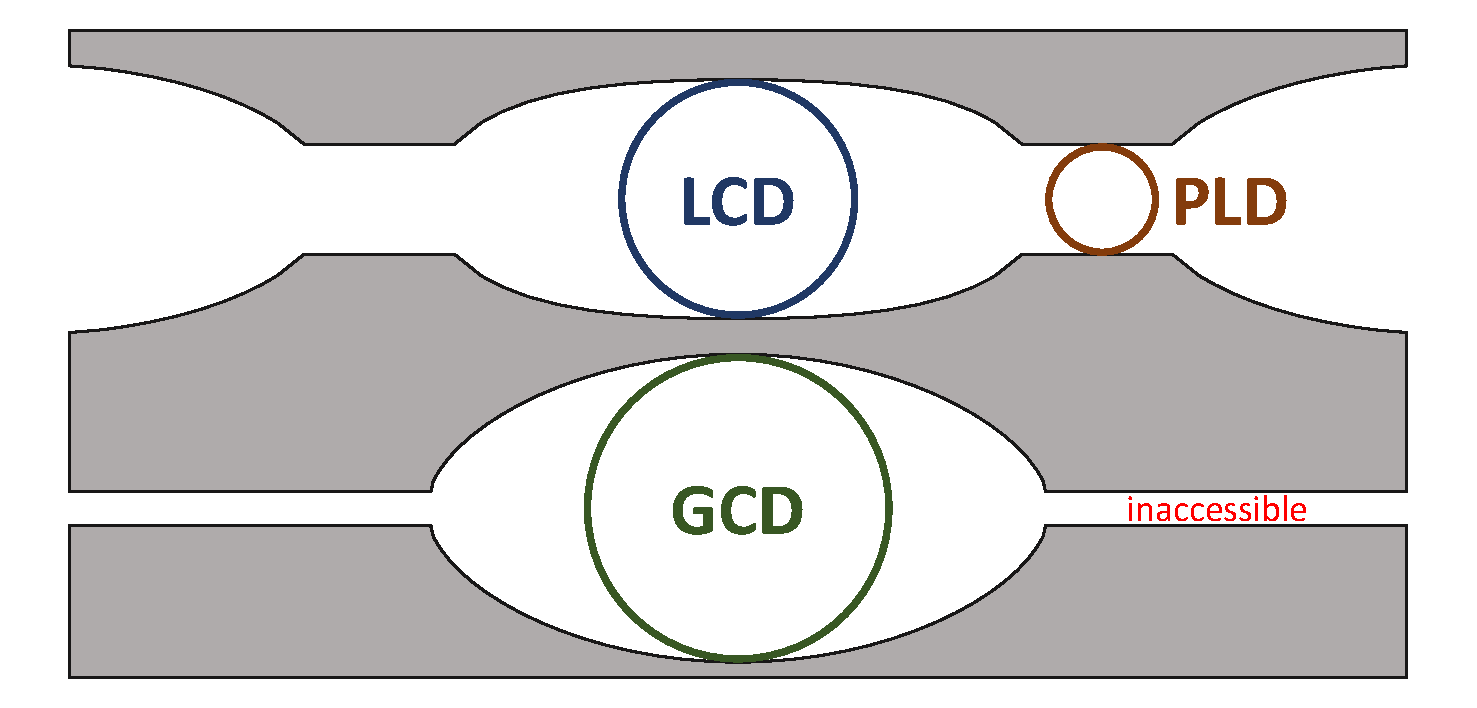
\includegraphics[width=0.65\textwidth]{figures/2-thermo/pores.pdf}
  \caption{Illustration of the different pore sizes D$_f$, D$_i$ and D$_{if}$. Note that in some materials D$_{if}$ is equal to D$_i$, when the largest included sphere is also accessible through a free diffusion path. }\label{fgr:pore_size}
\end{figure}

To define these pore sizes, it is necessary to first determine the radii of the framework atoms that shape the surrounding pores. These radii can be defined using different methods, with the default mode utilizing the Cambridge Crystallographic Data Centre's (CCDC) radii. This method is widely used in the literature. Additionally, this section introduces another set of radii based on the universal forcefield~\autocite{rappe1992}, which is used for all types of molecular simulations throughout this thesis. The determination of these radii are inspired by an approach developed by Hung et al.\autocite{Hung_2021} The atomic radii correspond to the distance at which the LJ potential reaches $3 k_\text{B} T/2$, for $T = \SI{298}{\kelvin}$. This definition enables easier comparison with the quantities obtained from molecular simulations. In case of ambiguity, different indices will be used to differentiate between the two methods. For instance, LCD\e{CCDC} corresponds to the standard definition of the LCD that utilizes the CCDC radii when running the Zeo++ software, while the LCD\e{UFF} is defined based on the atomic radii that is dependent on the UFF forcefield. In this chapter, I will mainly use the forcefield-based definition --- the largest cavity diameter denoted LCD\e{UFF} will be predominantly used, and the studies on void fraction and surface areas will also be defined using this set of radii.


\subsubsection{Surface area}

The surface areas are calculated using a random sampling technique across the surface of the different atom surfaces. The algorithm counts only the points that do not overlap with another atom. This allows for the calculation of an adsorbable surface for each atom. Ultimately, the surface area can be obtained by summing up all these surfaces. This algorithm, known as the ``rolling ball'' algorithm, was initially developed by Shrake and Rupley in 1973.\autocite{Shrake1973} The Voronoi tessellation determines the accessible and non-accessible areas of the structure by using a probe. Depending on the location of the surfaces, they are categorized as either accessible or non-accessible surface areas. In this chapter, the accessible surface area is defined using a probe of $1.2$~\si{\angstrom}. This value is computationally equivalent to the experimental \ce{N2} BET surface area.

\begin{figure}[ht!]
  \centering
  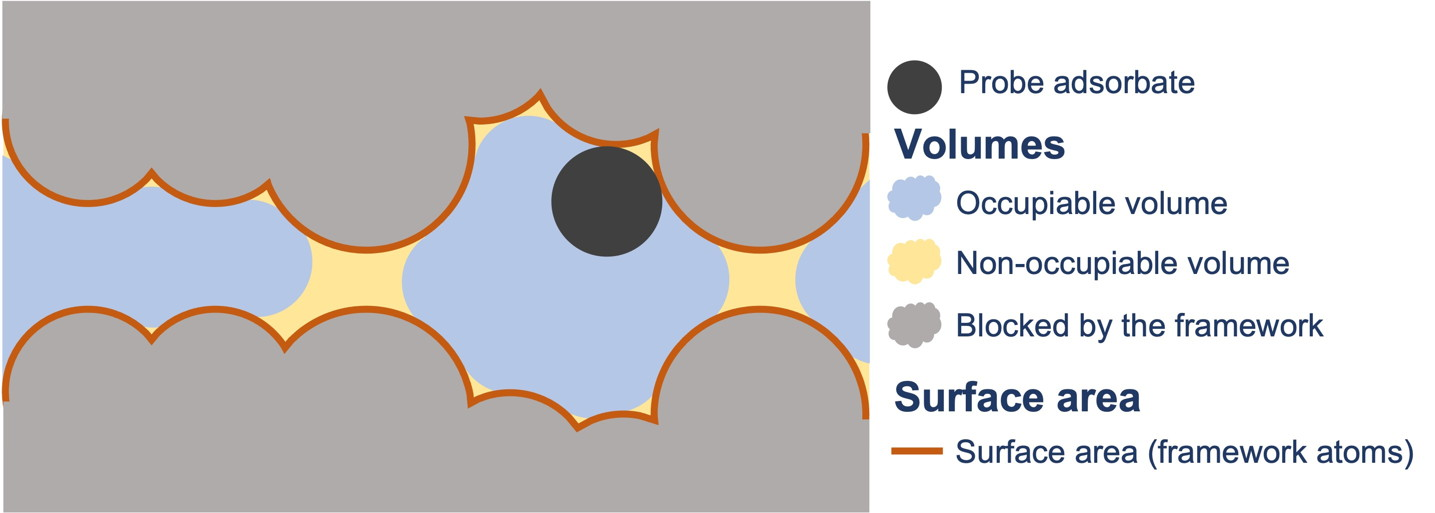
\includegraphics[width=0.65\textwidth]{figures/1-screening/Pore_descriptors.jpg}
  \caption{Illustration of the pore surface area and volume in a nanoporous material. As illustrated, there are different definitions of the pore volume: we can either consider the whole volume of the pores (occupiable+non-occupiable) or only the volume occupiable by a probe. People usually use the first definition, but the second definition has recently been proposed. Studies have shown that occupiable volume has a better accordance with experimental data.\autocite{vol_Ongari2017} The surface area also changes depending on the definition. \todo{à discuter}}\label{fgr:pores}
\end{figure}

\subsubsection{Pore volume and porosity}

The pore volume is calculated by randomly sampling the accessible and inaccessible Voronoi cells. Similarly, other algorithms perform a random sampling over a regular mesh. If the probe used for sampling does not overlap with a framework atom, then it is counted in the number of accessible points $N$ in the volume. The ratio of this number $N$ and the total number of points sampled gives the fraction of the pore volume, also known as the void fraction or porosity. By using the Voronoi decomposition, it is also possible to define the accessible and non-accessible Voronoi cells to reduce the space that needs to be sampled in a Monte Carlo simulation for the surface area and the void fraction calculations.


\subsection{Intermolecular interactions}\label{sct:interaction}

In most of the studies in this thesis, rigid structures interacting with guest adsorbates are considered. The intramolecular interactions will not play any significant role in the simulations, as the ionic, chemical, or metallic bonds between the atoms of a molecule are predefined at a specific set of distances and remain unchanged throughout the simulations. As discussed in the final chapter, this approximation can generate discrepancies between the theoretical model and the experimental observations. However, considering the goal of achieving screening approaches, such as the ones introduced in Chapter 1, adding flexibility in intramolecular interactions would significantly reduce the size of the database that can be screened. For these reasons, the term ``interaction energy'' will mainly refer to the guest--host and guest--guest intermolecular interactions --- host--host interactions would compromise the assumption of framework rigidity.

In classical theory of molecular physics, the intermolecular interactions can be categorized into three different types based on their strength: (i) the ion--dipole and ion--induced dipole interactions ($40$--$600$~\si{\kilo\joule\per\mol}), (ii) the hydrogen bonding ($10$--$50$~\si{\kilo\joule\per\mol}), and (iii) the van der Waals interactions ($1$--$10$~\si{\kilo\joule\per\mol}). It is important to note that these energy values are only indicative and the interaction depends on the nature of the molecules. However, they provide a ranking of the different forces according to their strength. Moreover, the ionic and covalent bonding is always stronger than any intermolecular interactions (over $100$~\si{\kilo\joule\per\mol}). The generic term ``van der Waals interactions'' actually encompasses three different concepts known as the Keesom, Debye and London interactions. The Keesom interaction focuses on the electrostatic interaction between permanent multipoles (representing the electronic density around the molecules),\autocite{keesom1915second} while the Debye induction force corresponds to the interaction between a multipole of a molecule and an induced multipole of another one.\autocite{Roberts_1938} The London dispersion interaction occurs between instantaneous multipoles created by natural fluctuations in the electron density around polarizable atoms.\autocite{london1930theorie,polanyi1932section} To quantify these interactions, it is possible to consider dipole interactions since they have the most influence in the multipole expansion of the electron density. The Keesom interaction potential $U\e{K}$ can therefore be reduced to the dipole--dipole interaction, which depends on the inverse third power of the distance for fixed dipoles. However, in fluid phases, the average over all angles is better described by the inverse sixth power, as shown in the equation~\ref{eq:keesom} below:
\begin{equation}\label{eq:keesom}
  U\e{K} = -\dfrac{\mu_1^2\mu_2^2}{{(4\pi\epsilon_0\epsilon_r)}^2r^6}\times\dfrac{2}{ 3k\e{B}T}
\end{equation}
where $\mu_1$ and $\mu_2$ are the dipole moments of the molecules $1$ and $2$, $\epsilon_0$ the vacuum dielectric permittivity and $\epsilon_r$ relative permittivity of the surrounding material, k\e{B} the Boltzmann constant, $T$ the temperature and $r$ the intermolecular distance. The Debye interaction potential $U\e{D}$ being reduced to the permanent dipole--induced dipole interactions can now be expressed using the electric polarizability $\alpha_1$ and $\alpha_2$ of the molecule $2$ as shown in equation~\ref{eq:debye}.
\begin{equation}\label{eq:debye}
  U\e{D} = -\dfrac{\mu_1^2\alpha_2 + \mu_2^2\alpha_1}{{(4\pi\epsilon_0\epsilon_r)}^2r^6}\times\dfrac{1}{k\e{B}T}
\end{equation}
Finally, the London dispersion interaction potential $U\e{L}$ is now the fluctuating dipole--induced dipole interaction and can be expressed as follows:
\begin{equation}\label{eq:london}
  U\e{L} = -\frac{\alpha_1\alpha_2}{{(4\pi\epsilon_0\epsilon_r)}^2r^6}\times\frac{3}{2}\times\frac{I_1 I_2}{I_1+I_2}
\end{equation}
where $I_1$ and $I_2$ are the first ionization energies. Note that the van der Waals potentials are all negative (attractive interaction) and depend on the inverse sixth power of the distance --- considering only the dipole moments. Before delving into the computational modelization of these long-distance intermolecular forces, it is necessary to specify the repulsive force that occurs at very short distances. This force can be explained by the Pauli exclusion principle, which states that electrons in both atoms cannot occupy the same quantum space.

For the system of interest, the adsorption of noble gases in nanoporous materials, the guest--guest and guest--host interactions can be described by the induction and dispersion interactions only. I will use a simple model, the Lennard-Jones (LJ) potential $U\ex{LJ}$,\autocite{LJ_1924} that relies on a repulsive term for the Pauli exclusion principle and an attractive term to model the attractive van der Waals component of the interaction, as shown below:
\begin{equation}\label{eq:LJ}
  U\ex{LJ} = 4\epsilon \left({\left(\dfrac{\sigma}{r}\right)}^{12} - {\left(\dfrac{\sigma}{r}\right)}^{6}\right)
\end{equation}
where $\epsilon$ is the depth of the well (minimal attractive energy) and $\sigma$ is the distance at which the potential is zero. The forcefield defines the LJ parameters $\epsilon$ and $\sigma$ for either all atom pairs or only for the same type of atoms. For the commonly used universal forcefield (UFF),\autocite{rappe1992} only the parameters for atoms of the same nature are defined and the parameters of the pair atoms can be induced using combining rules. In this thesis, I will use the UFF forcefield (as it performs well compared with \emph{ab initio} forcefields for \ce{CO2} and \ce{CH4} uptake values\autocite{McDaniel_2015}) and the Lorentz-Berthelot mixing rules to combine the LJ parameters --- it makes an arithmetic average of the $\sigma$ values (Lorentz rule) and a geometric one of the $\epsilon$ values (Berthelot rule). Finally, to reduce the computation time, one usually set a cutoff distance at which the LJ potential can be considered negligible. At this cutoff distance, one can apply a shift so that the energy equals zero at the cutoffs (discontinuity of energy), just truncate (discontinuity of the force), or use a tail switching function to make the tail converge smoothly to zero near the cutoff. In most of the simulations in my screening studies, I adopted a shifting strategy combined with a cutoff of \SI{12}{\angstrom}.

In adsorption simulations of other gas molecules with partial charges, it is usually necessary to calculate the Coulomb interaction between the partial charges of the host framework and those of the adsorbate --- in periodic systems, an Ewald summation is typically employed to account for this interaction. However, in the case of noble gases, such ion--dipole and dipole--dipole interactions do not exist due to the perfect neutrality of the molecules. Nevertheless, it can be argued that the ion--induced dipole can be adequately described by a simple LJ potential. To provide a comprehensive representation of the intermolecular interactions, the energy induced by the charges of the surrounding framework atoms should be added to the adsorbate. Several approaches have been developed in the literature to enhance the description of the intermolecular interactions by coupling LJ potentials with an induction potential,\autocite{Lachet_1998,Becker_2017} which are not used in my work.

To summarize this section on the modelization of the intermolecular interactions in the adsorption simulations, it is essential to highlight the main assumptions in the modelization that may impact the accuracy of the method. Firstly, the framework remains rigid throughout the simulation, which eliminates the need for molecular dynamics simulations of the framework to save time, but it also hides the effects of a known phenomenon.\autocite{Witman_2017} Secondly, the polarizability of the adsorbate is only partially considered, as the interaction with the charges of the framework is not taken into account. The difference in polarizability between xenon and krypton can be further exploited to enhance the selectivity, as suggested by experimental studies emphasizing the key role of polar groups and open metal sites.\autocite{Li_2019,Pei_2022,Perry_2014} Lastly, the complex induction and dispersion interactions are described using a two-parameter model. Although this model does not capture all the nuances of differences between the same atom in different environments, it is possible to fine-tune these parameters for very specific cases. However, in a screening strategy, some accuracy on specific cases can be sacrificed to improve the generalization error, as demonstrated by the good performance of the UFF forcefield on a large dataset.\autocite{McDaniel_2015}
These assumptions have been made to strike a balance between the computational speed and a detailed description of the physical phenomena at stake. Moreover, the focus this thesis is on the development of screening methodologies rather than molecular interaction modeling.


\subsection{Mixture adsorption: Grand Canonical Monte Carlo}\label{sct:GCMC}

%intro 
As previously discussed, adsorption can be viewed as a gas--solid or liquid--solid interfacial phenomenon. The adsorbate phase fills the accessible pore volumes depending on the physical conditions of the material. Predicting how adsorbates would interact with the pore surface, the maximum number of molecules that can fit, the most stable configuration, etc., is challenging and cannot be achieved through a simple model. To address these questions, it is necessary to evaluate all possible adsorption configurations each with a different number of adsorbate molecules, and then select the most thermodynamically plausible ones. This evaluation requires these configurations to follow a predefined probability distribution from statistical physics, such as the grand canonical ensemble probability, as it allows for the variation of the number of molecules (adsorbate molecules) and the total energy. By using a Monte Carlo simulation, it is possible to vary the energy and the loading inside the pores so that the distribution of configurations $c$ follows the probability law below: 
\begin{equation}\label{eq:gc}
  P_c = \dfrac{1}{\Xi}e^{-\beta\left(E_c-\mu N_c\right)} 
\end{equation}
where $E_c$ and $N_c$ are respectively the energy and the number of adsorbate particles in the configuration $c$. Normally the energy and the number of molecules of all particles should be considered, but for now, since the whole system is considered rigid, I will only focus on the adsorbate molecules. The chemical potential $\mu$ and the temperature $T$ ($\beta=1/k\e{B}T$) correspond to the ones of the gas phase in equilibrium with the adsorbent material. And the pressure and volume $V$ are considered fixed under the rigidity assumption. The grand canonical partition function $\Xi(\mu,V,T)$ will then be the following sum over all possible configurations: 
\begin{equation}
  \Xi(\mu,V,T) = \sum\limits_c e^{-\beta\left(E_c-\mu N_c\right)} 
\end{equation}
This multiplicative constant does not need to be known in the Monte Carlo simulation I will describe now. 

Beyond these theoretical considerations, the grand canonical Monte Carlo simulation which refers to a Metroplis-Hastings Monte Carlo algorithm in the context of the grand canonical thermodynamic ensemble, requires several key characteristics to fulfill the above-mentioned probability distribution of the configurations. Monte Carlo (MC) refers to the randomness inherent to gambling games at the eponymous casino on the azure coast of Monaco. In MC simulations, are therefore relying on randomly generating atomic configurations; but it is necessary to remain in the physically possible atomic space to the greatest extent, while exhaustively exploring all possible chemical configurations. 
Starting from an initial configuration $c_0$, the algorithm has different rational moves to change the configuration with a controlled degree of randomness. Some of these moves are illustrated in Figure~\ref{fgr:mc}. The second key algorithmic step (acceptance or rejection condition), introduced by Metropolis and co-workers, allows the reproduction of any distribution with an unknown multiplicative prefactor.\autocite{Metropolis1949} The configuration $c_1$ resulting from the random move is evaluated by calculating the transition probability (like in a Markov chain) or acceptance rate $acc(c_0 \rightarrow c_1)$: 
\begin{equation}
  acc(c_0 \rightarrow c_1) = \min\left(1, e^{-\beta\left(E_{c_1}-E_{c_0}-\mu \left(N_{c_1}-N_{c_0}\right)\right) }\right)
\end{equation}
The configuration $c_1$ is accepted if a number randomly drawn from the $[0,1]$ interval is higher than the acceptance rate $acc(c_0 \rightarrow c_1)$. For an acceptance rate of $1$, when $c_1$ is more stable than $c_0$ ($E_{c_1}-\mu N_{c_1}\leq E_{c_0}-\mu N_{c_0}$), the move is automatically accepted since by construction this randomly drawn number would be lower than $1$. On the other hand, if the move is rejected, then we generate another configuration $c_1$ using another random move, and the acceptance/rejection process restarts until a move is accepted. At the end of the $n$ cycles of the MC simulation, only the accepted configurations $\left\{c_0,\ldots,c_n\right\}$ form a Markov chain, and this sequence describes the probability distribution of the grand canonical ensemble described in equation~\ref{eq:gc}. The multiplicative prefactor does not influence the algorithm since the acceptance rate corresponds to ratios of probabilities $P_c$, so that no prior knowledge of the chemical space is needed, which is a valuable simplification.

\begin{figure}[ht]
  \centering
  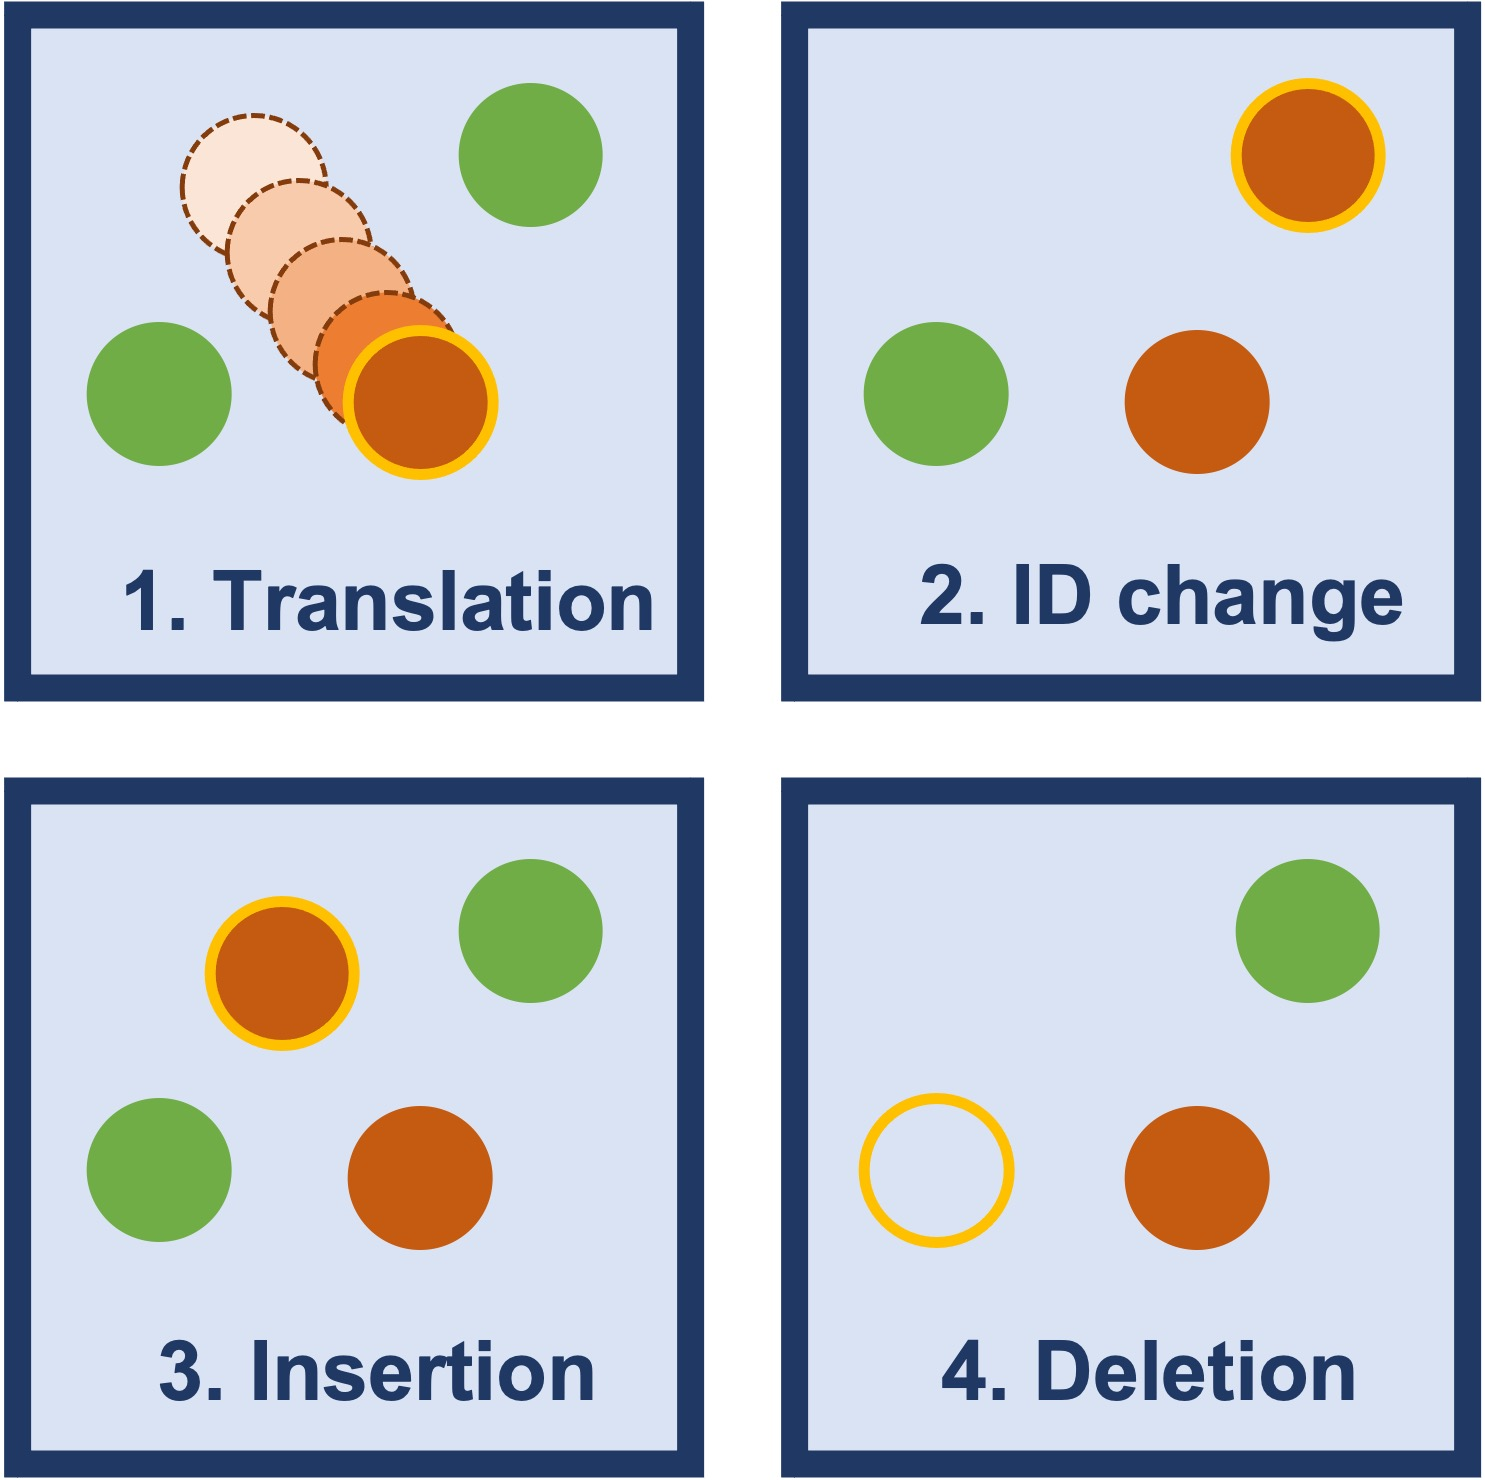
\includegraphics[width=0.99\textwidth]{figures/2-thermo/MC_moves.jpg}
  \caption{MC moves in a system of two types of monoatomic atoms (green and orange). The modification on the first box is highlighted by the yellow circle and the dragging pattern is represented by a set of dashed circles. The boxes 2 to 4 represent the moves going from the initial state represented in box 1, the corresponding move is highlighted by a yellow outer circle. All these moves are used in the GCMC calculations performed using the RASPA2 software. }\label{fgr:mc}
\end{figure}

To complete the description of the grand canonical Monte Carlo (GCMC) simulation, let us now consider the different MC moves used to generate a configuration from another. The probabiities of occurrence of these moves vary depending on the chosen parameterization. For monoatomic molecules, there are only four relevant moves (Figure~\ref{fgr:mc}): (i) translation of a randomly selected molecule with a displacement randomly chosen within a specific radius, (ii) conversion of the identity of a randomly chosen molecule to another one, (iii) insertion of an adsorbate molecule, and (iv) deletion of an adsorbate molecule. Rotations of the adsorbate are deliberately omitted due to the spherical symmetry of noble gases, and the change of volume is also dismissed since the flexibility of the material framework is not considered. In the GCMC screenings performed in this thesis, the probabilities of translation (i), of identity change (ii), of particle reinsertion ((iii) and (iv)) and of particle swap ((iii) or (iv)) are respectively $1/6$, $1/3$, $1/6$ and $1/3$. To clarify the terms used here, for a particle reinsertion, a particle is selected and moved randomly to another location; and for a particle swap, there is the same equal chances to insert a new molecule or to delete one. 

By using a GCMC algorithm, it is possible to generate a set of configurations according to their corresponding probability of occurrence. Since the probability law is directly derived from equation~\ref{eq:gc}, the series of configurations describe the thermodynamic equilibrium state of a nanoporous material in contact with a reservoir containing a xenon-krypton mixture at a given composition, pressure and temperature. Ensemble averaging enables the derivation of different thermodynamic quantities, such as the averaging loading or uptake at a given pressure (several pressures yield the isotherm) and the isosteric heat of adsorption for each adsorbate (Xe and Kr). The ratio of the uptakes $q$ informs on the selectivity $s$ of the thermodynamic separation process: 
\begin{equation}\label{eq:selec}
  \boxed{
  s = \dfrac{q\ex{Xe}}{q\ex{Kr}}\times\dfrac{y\ex{Kr}}{y\ex{Xe}}
  }
\end{equation}
where $y\ex{Xe}$ and $y\ex{Kr}$ designate respectively the mole fractions of Xe and Kr in the gas phase reservoir.

To characterize a separation process, it is theoretically sufficient to perform a GCMC calculation at every pressure, temperature and composition conditions. However, such simulations can be very time-consuming due to the need to extensively test insertion/deletion moves to accurately estimate the number of adsorbed molecules and the composition of the mixture. As a result, faster methods (machine learning) have been developed to estimate the selectivity at different physico-chemical conditions.\autocite{Simon_2015,Kang_2023} For the case of infinite dilution, faster methods are already available. One such method that will be introduced in the following subsection is the Widom insertion, which enables the estimation of adsorption performances at infinite dilution by estimating the Henry adsorption constant.


\subsection{Infinite dilution adsorption: Widom insertion}\label{sct:widom}

In 1963, B. Widom introduced a simple method for calculating thermodynamic properties in materials or fluid mixtures.\autocite{Widom1963} This method typically allows accessing to the difference of internal energy before and after the insertion of a test particle while keeping all other particles fixed, thereby comparing the N-particle and (N+1)-particle states. This energy difference $\Delta \Phi$ can then be used to deduce the excess free energy associated with the insertion $\Delta F\e{exc} = -k\e{B} T \ln\left(\langle \exp(- \beta\Delta \Phi) \rangle\right)$ by averaging the Boltzmann factors, which corresponds to the excess chemical potential induced by the addition of a particle. More precisely, the average is theoretically performed for all possible positions of the inserted particle; in practice, the tridimensional space is uniformly and randomly sampled until convergence of the value of $\Delta F\e{exc}$. In the domain of fluid phase equilibrium, Widom insertion is the most straightforward method to calculate chemical potential values. However, it has limitations in liquid-like phases where the insertable space is very narrow, and no relaxation is implemented to account for the reorganization of surrounding particles.\autocite{Nezbeda_1991} 

This thesis will only focus on the insertion from 0 to 1 particle, where no issues of overlap between adsorbate particles occur. In this low-loading limit, Widom insertion is simply a random insertion of an adsorbate into an empty nanoporous framework. By randomly sampling the void space, a distribution of interaction energies $\mathcal{E}\e{int}$ can be obtained. The average of the Boltzmann weights associated with these energies is directly proportional to the adsorption free energy $\Delta G\e{ads}$ and the Henry adsorption constant $K\e{H}$. By taking the Boltzmann average of the interaction energies, the adsorption enthalpy $\Delta H\e{ads}$ can also be computed. It should be noted that these quantities remain valid only at infinite dilution, and for higher quantities of adsorbates, the previously described GCMC technique should be used. If the sampling is thorough enough, it is possible to derive the following definitions of $\Delta G\e{ads}$ (equation~\ref{eq:ads_gibbs}), $K\e{H}$ (equation~\ref{eq:henry}) and $\Delta H\e{ads}$ (equation~\ref{eq:ads_enthalpy}) based on a complete sampling of the interaction energies $\mathcal{E}\e{int}$ in all points of the space. 

\subsubsection{Adsorption Gibbs free energy}

The adsorption Gibbs free energy $\Delta G\e{ads}$ is equal to the excess free energy previously calculated in a Widom insertion as the structure is rigid and $PV$ does not fluctuate ($G = F + PV$). 

\begin{equation}\label{eq:ads_gibbs}
  \boxed{
  \Delta G\e{ads} = -RT \ln\left(\langle \exp(-\mathcal{E}\e{int}/RT) \rangle\right)
  }
\end{equation}

\subsubsection{Henry constant}

To derive the Henry constant $K\e{H}$, let us consider an ideal gas in the bulk phase. The number of adsorbed molecules $n\e{ads}$ can then be expressed using the bulk density of the adsorbate molecule $\rho\e{ads,bulk}$ and the volume of the pores $V\e{pore}$:

\begin{equation}\label{eq:1}
    n\e{ads} = \rho\e{ads,bulk} \times V\e{pore}  
\end{equation}

The pore volume can be seen as the continuous sum of each voxel times the Boltzmann probability of presence, which is represented by the following integral of the Boltzmann factors. This integral can then be changed to the average of the Boltzmann factors:

\begin{equation}\label{eq:vpore}
    V\e{pore} = \int_V \exp\left(- \mathcal{E}\e{int}(\textbf{r})/RT\right) d\textbf{r} = V \langle \exp\left(-\mathcal{E}\e{int}/RT\right) \rangle
\end{equation}

Let us apply equation~\ref{eq:vpore} and the perfect gas equation of state $P = \rho\e{ads,bulk}RT$ on the bulk gas in equilibrium. The equation~\ref{eq:1} can be simplified as

\begin{equation}
    \dfrac{n\e{ads}}{V} = \dfrac{P}{RT} \langle \exp\left(-\mathcal{E}\e{int}/RT\right) \rangle
\end{equation}

By considering the gravimetric loading $L\e{ads}$ (in~\si{\milli\mole\per\gram}) instead of absolute value, we need to divide the equation by the mass density of the framework $\rho_f$:

\begin{equation}
  L\e{ads} = \dfrac{n\e{ads}}{V\rho_f} = \dfrac{\langle \exp\left(-\mathcal{E}\e{int}/RT\right) \rangle}{\rho_f RT} P
\end{equation}

Since the Henry's law is described by $L\e{ads}=K\e{H} \times P$, we have the final relationship between the Henry adsorption constant and interaction energy distribution. If we consider a mixture, the pressure should be replaced by partial pressures.

\begin{equation}\label{eq:henry}
    \boxed{
    K\e{H} = \dfrac{\langle \exp\left(-\mathcal{E}\e{int}/RT\right) \rangle}{\rho_f RT} = \dfrac{1}{\rho_f RT} \exp\left(-\dfrac{\Delta G\e{ads}}{RT}\right)
    }
\end{equation}

Note that the $\rho_f$ factor comes from the use of a gravimetric loading expressed in~\si{\milli\mole\per\gram} and is not always present in the different derivations of the literature.\autocite{PoreBlazer} The $RT$ factor derives from the perfect gas assumption made in equation~\ref{eq:1}, which is a good approximation in the case of noble gas. 


\subsubsection{Adsorption enthalpy or heat of adsorption}

Finally, if we consider an adsorption equilibrium (e.g., $\text{Xe}\e{(g)} \rightleftharpoons \text{Xe}\e{(ads)}$), we can define an equilibrium constant $K\e{ads}$ based on the thermodynamic activities (partial pressure for a gas and volumetric loading for an adsorption phase) of the adsorbate in the different phases:
\begin{equation}
  K\e{ads} = \dfrac{l\e{ads}P^o}{y\e{gas}Pc^o}
\end{equation}
where $l\e{ads}=n\e{ads}/V$ is the volumetric loading in the adsorbed phase (similar to a molar concentration) and $y\e{gas}$ the mole fraction in the gas phase for a given compound (e.g., Xe), and $P^o$ is the standard pressure. And, here we assume the gas ideal by taking a fugacity coefficient of $1$. For a gas at infinite dilution, the Henry's law can then be applied to derive the following relation:

\begin{equation}\label{eq:eq_cst}
  K\e{ads} = \dfrac{n\e{ads}P^o}{y\e{gas}PVc^o} = \dfrac{K\e{H}y\e{gas}P\rho_f V P^o}{y\e{gas}PVc^o} = \dfrac{K\e{H}\rho_f P^o}{c^o} = \dfrac{\langle \exp\left(-\mathcal{E}\e{int}/RT\right) \rangle}{c^o RT/P^o}
\end{equation}
As a sanity check, we can verify that $c^o/P^o$ has a unit homogeneous with a molar energy, which is consistent with $K\e{ads}$ being unitless.

Now by applying the Van't Hoff equation to this infinite-dilution adsorption equilibrium constant $K\e{ads}$, we can derive an expression of the adsorption enthalpy at infinite dilution:

\begin{equation}
  \Delta H\e{ads} = -R\dfrac{\dd \ln\left(K\e{ads}(T)\right)}{\dd (1/T)}
\end{equation}

Then by decomposing the logarithm on the fraction of equation~\ref{eq:eq_cst}, 
\begin{equation}
  \Delta H\e{ads} = \dfrac{\dd \ln\left(c^o R/P^o\right)}{\dd (1/T)} - R\dfrac{\dd \ln\left(\langle \exp\left(-\mathcal{E}\e{int}/RT\right) \rangle\right)}{\dd (1/T)} - R\dfrac{\dd \ln\left(1/T\right)}{\dd (1/T)}
\end{equation}

Then, as $c^o R/P^o$ is constant for the variable $T$, the expression can be simplified to two terms, the first one being the logarithmic derivative of itself ($1/T$) and the second term is the logarithmic derivative of the sum of the exponential terms. 

\begin{equation}
  \Delta H\e{ads} = 0 - R\dfrac{\dd \ln\left(\langle \exp\left(-\mathcal{E}\e{int}/RT\right) \rangle\right)}{\dd (1/T)} - RT
\end{equation}

Using the property that the logarithmic derivative of a function $f$ is obtained by the formula $\dfrac{\dd \ln\left(f\right)}{\dd x}=f'/f$, we can calculate the derivative of the average of the Boltzmann factors $\langle \exp\left(-\mathcal{E}\e{int}/RT\right) \rangle$:

\begin{equation}
  \Delta H\e{ads} = -R\dfrac{1}{\frac{1}{N}\sum e^{-\frac{\mathcal{E}\e{int}}{RT}}} \frac{1}{N}\sum \dfrac{\dd \exp\left(-\mathcal{E}\e{int}/RT\right)}{\dd (1/T)} - RT
\end{equation}
where N corresponds to the number of points where the Widom particle has been inserted.
The exponential derivative makes the energy factors come out, and we obtain the following expression:
\begin{equation}
  \Delta H\e{ads} = -R\dfrac{1}{\sum e^{-\frac{\mathcal{E}\e{int}}{RT}}} \sum - \frac{\mathcal{E}\e{int}}{R} e^{-\frac{\mathcal{E}\e{int}}{RT}} - RT
\end{equation}

With some simplification, the adsorption enthalpy $\Delta H\e{ads}$ can be expressed as the Boltzmann average of the interaction energies minus a term $RT$ that corresponds to the internal energy in the bulk phase under the ideal gas assumption (perfect gas equation of state).

\begin{equation}\label{eq:ads_enthalpy}
  \boxed{
  \Delta H\e{ads} = \dfrac{\sum \mathcal{E}\e{int}e^{-\frac{\mathcal{E}\e{int}}{RT}}}{\sum e^{-\frac{\mathcal{E}\e{int}}{RT}}} - RT
  }
\end{equation}

The isosteric heat of adsorption $q\e{st}$ is then simply the opposite of the adsorption enthalpy, at infinite dilution. 

\subsubsection{Adsorption entropy}

% entropy from free energy and enthalpy
From the values of the adsorption free energy and enthalpy, we can now deduce the adsorption entropy $\Delta S\e{ads}$ using the definition of the Gibbs free energy ($G = H-TS$):
\begin{equation}\label{eq:ads_entropy}
  \boxed{
  \Delta S\e{ads} = \dfrac{1}{T} \left(\Delta H\e{ads} - \Delta G\e{ads} \right)
  }
\end{equation}

\subsubsection{selectivity}

%selectivity
In the thesis, the selectivity is defined as the ratio of the proportion of Xe/Kr in the adsorption phase to the proportion in the gas phase in equation~\ref{eq:selec}. At infinite dilution, the selectivity can be rewritten using the Henry's law ($q\ex{i}=V\rho_f K\e{H}\ex{i}y\ex{i}P/n\e{tot}$) and simplifying the constant term $PV\rho_f/n\e{tot}$:
\begin{equation}\label{eq:selec_0}
  \boxed{
  s = \dfrac{K\e{H}\ex{Xe}y\ex{Xe}}{K\e{H}\ex{Kr}y\ex{Kr}}\times\dfrac{y\ex{Kr}}{y\ex{Xe}} = \dfrac{K\e{H}\ex{Xe}}{K\e{H}\ex{Kr}}
  }
\end{equation}
By extrapolating at the zero loading regime, the Xe/Kr selectivity can be simply expressed as the ratio of the Henry adsorption constants of xenon and krypton.

This section has simple thermodynamic quantities such as the adsorption Gibbs free energy, enthalpy and entropy from the study of a simple adsorption equilibrium equation. The following section will explore a thermodynamic characterization of the adsorption-based separation process by using another equilibrium. 

\subsection{The thermodynamics behind adsorption-based separation}\label{sct:thermo}

Now that the main simulation tools used to describe the competing adsorption of Xe/Kr binary mixtures have been introduced, let us rationalize the separation process by modeling the process within a hypothetical ``exchange'' equilibrium that corresponds to the exchange of gas phase Xe and Kr on a model adsorption site representing all the most attractive sites for a given pressure condition:
\begin{equation}\label{eq:exchange}
    \text{Xe}_{\text{(g)}} + \text{Kr}_{\text{(ads)}}
    \rightleftharpoons \text{Xe}_{\text{(ads)}} + \text{Kr}_{\text{(g)}}
\end{equation}

At any pressure and for a given composition, the equilibrium constant associated with equation~\ref{eq:exchange} is simply the selectivity $s$, defined in equation~\ref{eq:selec}, as the gas phase activities of $\text{Xe}_{\text{(g)}}$ and $\text{Kr}_{\text{(g)}}$ correspond to the partial pressures $y\ex{Xe}$ and $y\ex{Kr}$, while the adsorption phase activities of $\text{Xe}_{\text{(ads)}}$ and $\text{Kr}_{\text{(ads)}}$ correspond to their mole fractions $q\ex{Xe}$ and $q\ex{Kr}$. 

\subsubsection{Exchange Gibbs free energy}

The Gibbs free energy at equilibrium can be directly defined using the equilibrium constant. Applying this relation to the exchange equilibrium, it is possible to define an exchange Gibbs free energy $\Delta\e{exc}G$:
\begin{equation}\label{eq:exc_gibbs_free_energy}
  \boxed{
  \Delta\e{exc}G = -RT \ln\left(s\right)
  }
\end{equation}

\subsubsection{Exchange enthalpy}

This exchange equilibrium can be viewed as the substraction between the adsorption equilibria of xenon and krypton. Applying Hess's law of constant heat summation, we can derive an expression for the exchange enthalpy as the difference of the adsorption enthalpies between xenon and krypton within the mixture. 
\begin{equation}
  \boxed{
  \Delta\e{exc}H\ex{Xe/Kr} = \Delta\e{ads}H\ex{Xe} - \Delta\e{ads}H\ex{Kr}
  }
\end{equation}

Moreover, the adsorption enthalpy $\Delta\e{ads}H$ is generally defined by comparing the average energy difference between systems differing by one adsorbate:
\begin{equation}\label{eq:enthalpy_gen_def}
  \Delta\e{ads}H = \langle E \rangle\left(\langle N \rangle+1\right)-\langle E \rangle\left(\langle N \rangle\right) - RT
\end{equation}

In a GCMC calculation, we do not use the previous equation as it is, but we use a formula derived from the fluctuation theorem in statistical mechanics (see a complete derivation in this online article~\autocite{github_simon_gcmc}):
\begin{equation}\label{eq:ads_heat_gcmc}
  \Delta\e{ads}H\ex{Xe} \simeq \frac{\partial \langle E \rangle}{\partial \langle N \rangle} - RT = \frac{\partial\langle E \rangle}{\partial\langle \beta\mu \rangle} \bigg/ \frac{\partial \langle N \rangle}{\partial \langle \beta\mu \rangle} - RT = \dfrac{\langle EN \rangle - \langle E \rangle\langle N \rangle}{\langle N^2 \rangle - \langle N \rangle^2} - RT
\end{equation}
where $E$ corresponds to the total energy of the adsorption system and $N$ the total number of adsorbates at every step of the simulation. Note that this equation remains only valid for $N\gg1$, as the first step of the derivation is based on a first order Taylor expansion $\langle E \rangle\left(\langle N \rangle+1\right)-\langle E \rangle\left(\langle N \rangle\right) \simeq \frac{\partial \langle E \rangle}{\partial \langle N \rangle}$. 


On the other hand, at infinite dilution, we can derive back the equation~\ref{eq:ads_enthalpy} using equation~\ref{eq:enthalpy_gen_def}, where for $N\rightarrow0$ we now have $\Delta H\e{ads} = \langle E \rangle(1)-\langle E \rangle(0) - RT$. The average energy with one adsorbate minus the average energy without adsorbate corresponds to the average over the whole space of the guest--host interaction energies for one adsorbate particle (the host-host energy being encompassed in $\langle E \rangle(0)$). This expression of the adsorption enthalpy echoes with the one derived in equation~\ref{eq:ads_enthalpy}.

\subsubsection{Exchange entropy}

Now that the exchange Gibbs free energy and an exchange enthalpy have been defined at any pressure, the same approach can be applied as in equation~\ref{eq:ads_entropy} to derive the exchange entropy:
\begin{equation}\label{eq:exc_entropy}
  \boxed{
  \Delta\e{exc}S = \dfrac{1}{T}\left(\Delta\e{exc}H - \Delta\e{exc}G\right)= \dfrac{1}{T}\Delta\e{exc}H + R\ln(s)
  }
\end{equation}

\subsubsection{Conclusion}

Before concluding this methodological section, it is important to note that the thermodynamic quantities associated with the newly defined adsorption exchange equilibrium can be defined at different pressure, temperature and chemical composition conditions. Moreover, various methodologies can be used to calculate them. At infinite dilution, Widom insertions and the adsorption free energies and enthalpies are typically used to deduce the adsorption free energies and enthalpies and the exchange quantities associated with them. At higher pressures, GCMC calculations are necessary to define the free energy (via the loading values) and the isosteric adsorption heat. The following study will focus solely on two characteristic pressures: the ambient pressure (at \SI{1}{\atm}) and the limit of zero loading (infinite dilution). At \SI{1}{\atm}, the previously defined quantities will be denoted with an index $1$ to distinguish them from the infinite dilution case where an index $0$ will be used. For example, $\Delta\e{ads}H\e{1}\ex{Xe/Kr}$, $\Delta\e{exc}G\e{1}\ex{Xe/Kr}$ or $s\e{1}\ex{Xe/Kr}$ at \SI{1}{\atm}, and $\Delta\e{ads}H\e{0}\ex{Xe/Kr}$, $\Delta\e{exc}G\e{0}\ex{Xe/Kr}$ or $s\e{0}\ex{Xe/Kr}$ at the low-pressure limit. 

As for the simulations details, it is worth mentioning that for the GCMC calculations and Widom insertions, the RASPA2 software, developed by Dubbeldam et al.\autocite{dubbeldam2016}, was used. The intermolecular van der Waals interactions were described by a Lennard-Jones (LJ) potential with a cutoff distance of \SI{12}{\angstrom}. The LJ parameters of the framework atoms were obtained from the universal forcefield (UFF),\autocite{rappe1992} while the LJ parameters for the guest atoms (xenon and krypton) were taken from a previous screening study.\autocite{Ryan_2010} All the MOFs described in this study were taken from the CoRE MOF 2019 database.\autocite{Chung_2019}

%%%%%%

\section{Preliminary analyses of the separation performance}

The previous chapters showed how the computational screening of the nanoporous materials --- both existing frameworks and hypothetical structures --- for targeted adsorption properties has been a subject of extensive research. Several high-throughput screening studies have particularly focused on noble gas separation, and Xe/Kr separation. In addition to the testing and validation of methodological developments, large-scale studies have generally aimed to achieve one of three main objectives: (i) identify top performing materials for synthesis and/or characterization; (ii) better understand the limits of possible performance, and the relationships and trade-offs between various metrics of performance (selectivity, uptake, etc.); (iii) identify structure--property relationships by analyzing correlations between separation performance and structural properties of the materials, which provides chemical intuitions on designing better-performing materials. In this initial screening study of the thermodynamic quantities, I performed a screening of approximately 9\,700 tridimensional structures of a preprocessed version of the CoRE MOF 2019-ASR (all solvent removed) database that are publicly available --- only the non-disordered structures and the structures with a cell volume smaller than \SI{20}{\nano\meter\cubed} (to limit the overall calculation time) were considered. The focus of this study is to explore different relationships between Xe/Kr selectivity and structural descriptors based on geometrical analyses, as well as different thermodynamic descriptors (free energy, enthalpy, entropy). Some results have already been published in a scientific article~\cite{Ren_2021}.

\subsection{Structure--selectivity relationships}\label{sct:geometry}

An adsorption separation process is primarily characterized by a pivotal performance metric, known as the selectivity, as defined in equations~\ref{eq:selec} and~\ref{eq:selec_0}. To characterize materials that are likely to exhibit selectivity for a 20:80 Xe/Kr mixture separation (to compare with most literature screenings on a mixture extracted from the air), this selectivity was compared to geometrical descriptors calculated by the Zeo++ software\autocite{Zeo++}. Three structural descriptors have been computed: the accessible surface area of a \ce{N2}-sized probe of \SI{1.2}{\angstrom}, the void fraction occupiable by a \SI{2.0}{\angstrom} radius probe (roughly the size of a xenon),\autocite{vol_Ongari2017} and the diameter of the largest included sphere (D$_i$) using specially designed atom radii. Inspired by a recent work on the comparison of pore limiting diameters and self-diffusion coefficients,\autocite{Hung_2021} a list of van der Waals radii was defined to be used in the Zeo++ software.\footnote[1]{A code can be found at \url{https://github.com/eren125/zeopp_radtable}} In all Zeo++ calculations, an atomic radius was chosen based on the distance where the LJ potential reaches $3 k\e{B} T/2$, for $T = \SI{298}{\kelvin}$.

\subsubsection{Xenon uptake and selectivity}

Before delving deeper into the structure--selectivity relationship, the relation between the xenon uptake (the number of adsorbed xenon in the GCMC simulation) and the selectivity at \SI{1}{\atm} will be described. For instance, the xenon uptake is a crucial factor in the separation process, as it defines the working capacity of xenon produced through adsorption/desorption cycles. Figure~\ref{fgr:3D_uptake} reveals the possibility to have materials with a very high xenon uptake and a moderately high selectivity, or with very high selectivity but associated lower uptakes. Materials can exhibit selectivity values exceeding $100$ with Xe uptake around \SI{3}{\milli\mole\per\gram}, whereas an uptake exceeding \SI{6}{\milli\mole\per\gram} can only be obtained for selectivity values between $10$ and $20$. It becomes evident that maximizing both uptake and selectivity metrics simultaneously is challenging, and a trade-off must be made when designing nanoporous materials for xenon/krypton separation.\autocite{Zhang_2022} Various strategies, such as the adsorbent performance score (APS),\autocite{Solanki_2020} have been implemented to optimize both metrics using mixed metrics.
This trade-off can be rationalized by using the different structural descriptors (pore size, surface area and volume) introduced earlier. 

\begin{figure}[ht]
  \centering
  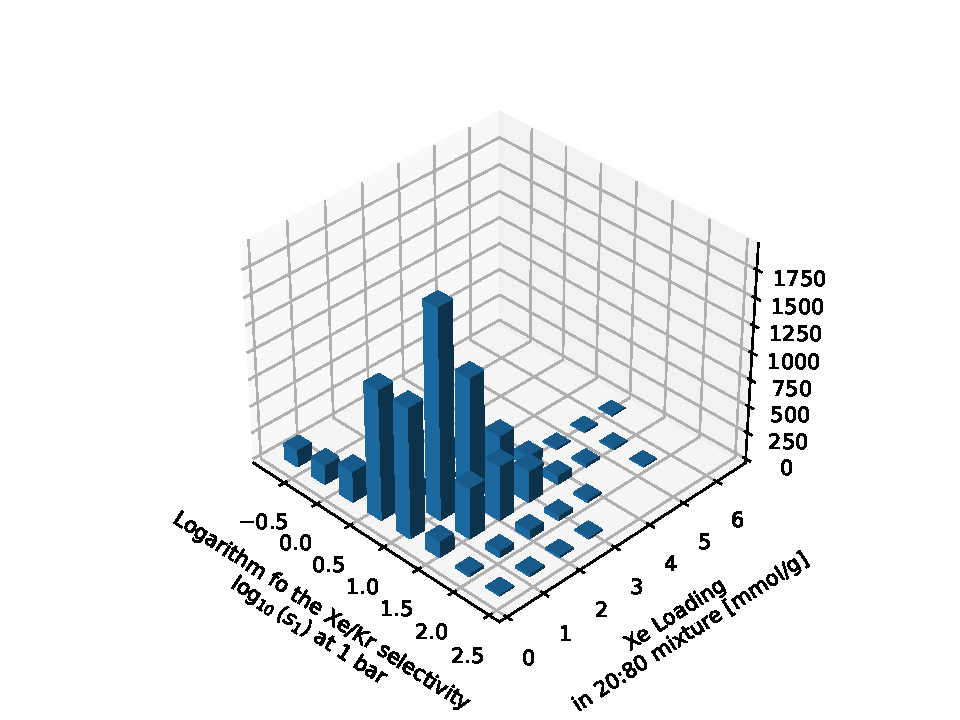
\includegraphics[width=0.5\textwidth,trim={2cm 0 2cm 2cm},clip]{figures/2-thermo/3D_hist_selec_uptake.pdf}
  \caption{3D histograms of in a bidimensional space formed by the Xe/Kr selectivity and the xenon uptake. The z-axis represents the number of structures with characteristics close to the one specified in x and y-axis. A base-10 logarithm has been applied to the selectivity values.}\label{fgr:3D_uptake}
\end{figure}
%check ordre figures

Furthermore, in the optimization of either xenon uptake or Xe/Kr selectivity, it is important to note that the best materials for each of these metrics are very rare within a given diverse dataset. The histogram shown in Figure~\ref{fgr:3D_uptake} demonstrates this scarcity, with a very low number of highly selective materials and high-capacity materials. The most frequently observed materials typically have a selectivity ranging from $1$ to $10$ and an uptake below \SI{3}{\milli\mole\per\gram}. These values can be considered as standard values for nanoporous material used in Xe/Kr separation, serving as reference values for comparing various performance metrics and building a chemical intuition. Therefore, a selectivity exceeding $20$ is considered relatively high (even though top-performing materials have a much higher selectivity\autocite{Pei_2022}) and a xenon uptake exceeding \SI{4}{\milli\mole\per\gram} indicates a significant adsorption capacity. The scarcity of these top-performing materials gives rise to the analogy of searching for a needle in a haystack, prompting some computational studies to design algorithms that focus on identifying the best materials rather than equally describing all materials.\autocite{Deshwal_2021,Glasby_2021} 

\subsubsection{Surface area and selectivity}

\begin{figure}[ht!]
  \centering
  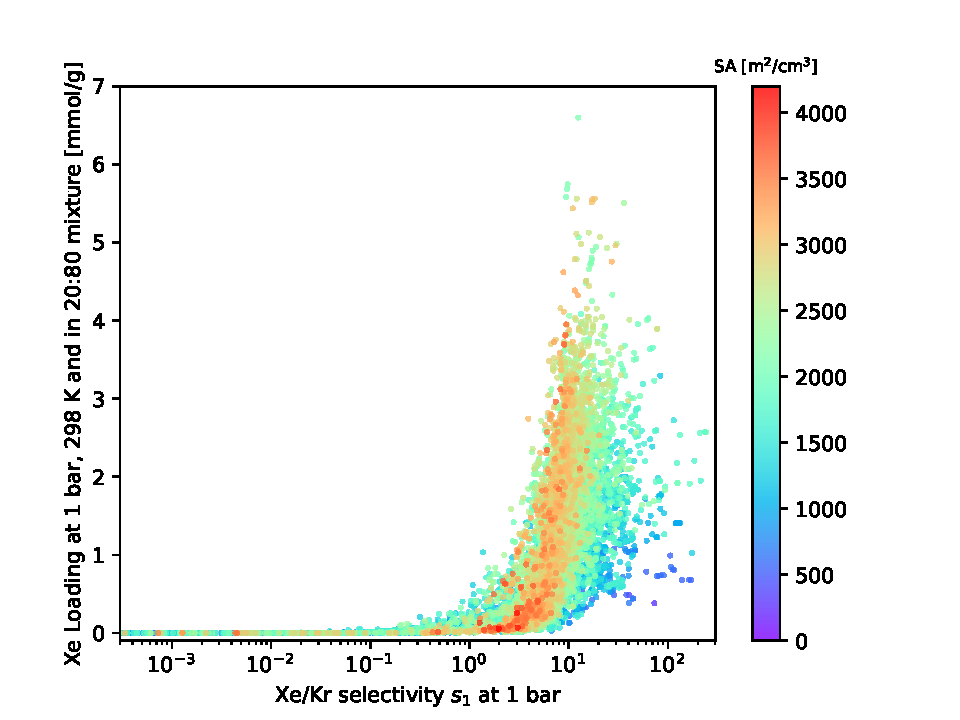
\includegraphics[width=0.48\textwidth]{figures/2-thermo/Scatterplot_uptake_selectivity_sa.pdf}
  \hfill
  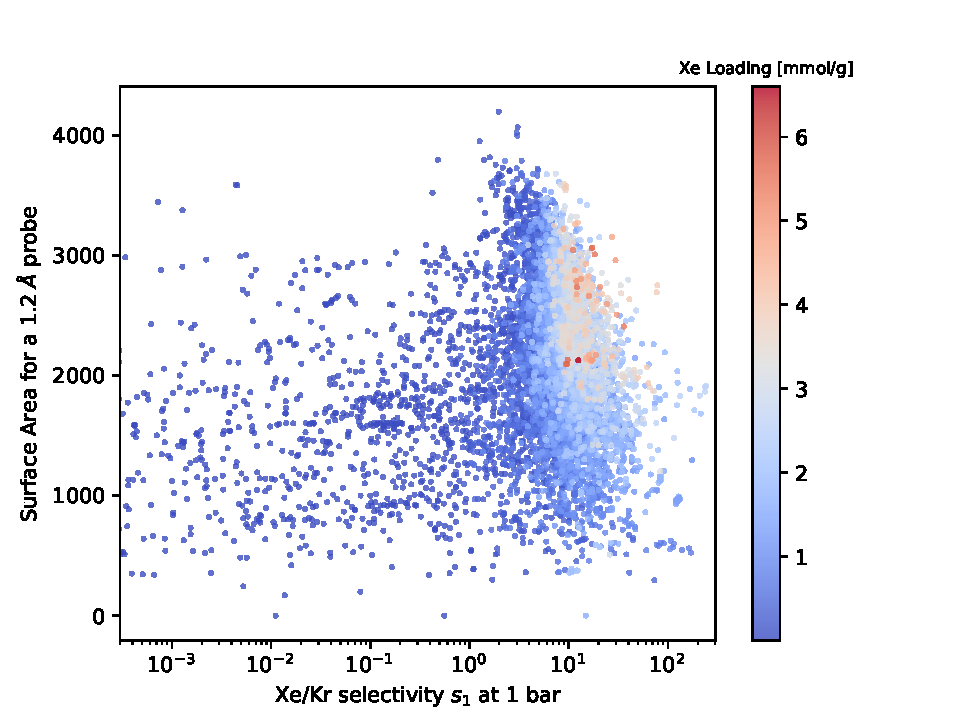
\includegraphics[width=0.48\textwidth]{figures/2-thermo/Scatterplot_sa_selectivity.pdf}
  \caption{On the left: scatterplot of the xenon uptake as a function of the selectivity and labeled by the values of the surface area. On the right: scatterplot of the selectivity and the surface area labeled by the quantity of xenon adsorbed. The selectivity and uptake are calculated by a GCMC simulation of a 20:80 Xe/Kr mixture.}\label{fgr:sa}
\end{figure}

Studies on methane storage applications, conducted by Wilmer et al.\autocite{Wilmer_2012} and by Fernandez et al.\autocite{Fernandez_2013}, have shown that methane uptake reaches its maximum within a specific optimal range of surface area values ($2500$-$3000$~\si{\square\meter\cubic\centi\meter}). Increasing the surface area beyond the range does not lead to higher values of methane uptake. This limitation is also observed for the Xe/Kr  selectivity, as shown in the right plot of the Figure~\ref{fgr:sa}. Materials with a selectivity around $5$ tend to have surface areas ranging from $0$ to $4000$~\si{\square\meter\cubic\centi\meter}, while those with a selectivity above $40$ tend to have a surface area below $2500$~\si{\square\meter\cubic\centi\meter}. On the other hand, the optimal surface area for xenon uptake falls between $2000$ and $3000$~\si{\square\meter\cubic\centi\meter}. It is evident that the relationship between selectivity and surface area is highly complex, and a precise range of surface areas does not guarantee high selectivity. Other structural descriptors need to be considered in conjunction with this descriptor to fully characterize selectivity. 

The 3D histogram in Figure~\ref{fgr:3D_hist_sa_vol} provides a visual representation of the surface area distribution for different selectivity categories. For selectivity values higher than $92$, the surface areas are mostly below $2000$~\si{\square\meter\cubic\centi\meter}. In the range of $92$ to $35$ selectivity, the distribution extends slightly wider, reaching up to $2500$~\si{\square\meter\cubic\centi\meter}. For selectivity values between $35$ and $13$, the interval spans a larger range, up to $3500$~\si{\square\meter\cubic\centi\meter}, but remains centered predominantly between $1000$ and $2500$~\si{\square\meter\cubic\centi\meter}. This split view of the distributions provides a better understanding of the characteristics of the best materials. However, it is important to note that surface area is not a deterministic variable as it is not possible to deduce selectivity based on surface area alone. A surface area between $500$ and $1000$~\si{\square\meter\cubic\centi\meter} may have a relatively high chance of exhibiting selectivity, but it encompasses a large number of materials and is even more likely to have selectivity values between $5$ and $35$ rather than values higher than that. 
\begin{figure}[ht!]
  \centering
  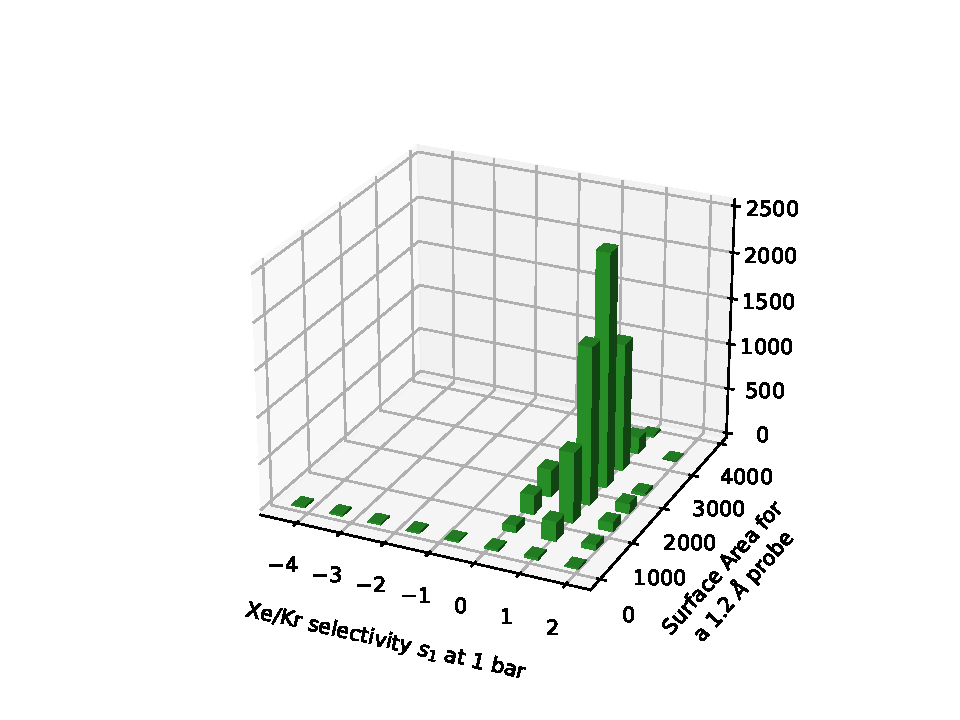
\includegraphics[width=0.48\textwidth,trim={2cm 0 2cm 2cm},clip]{figures/2-thermo/3D_hist_selec_SA.pdf}
  \hfill
  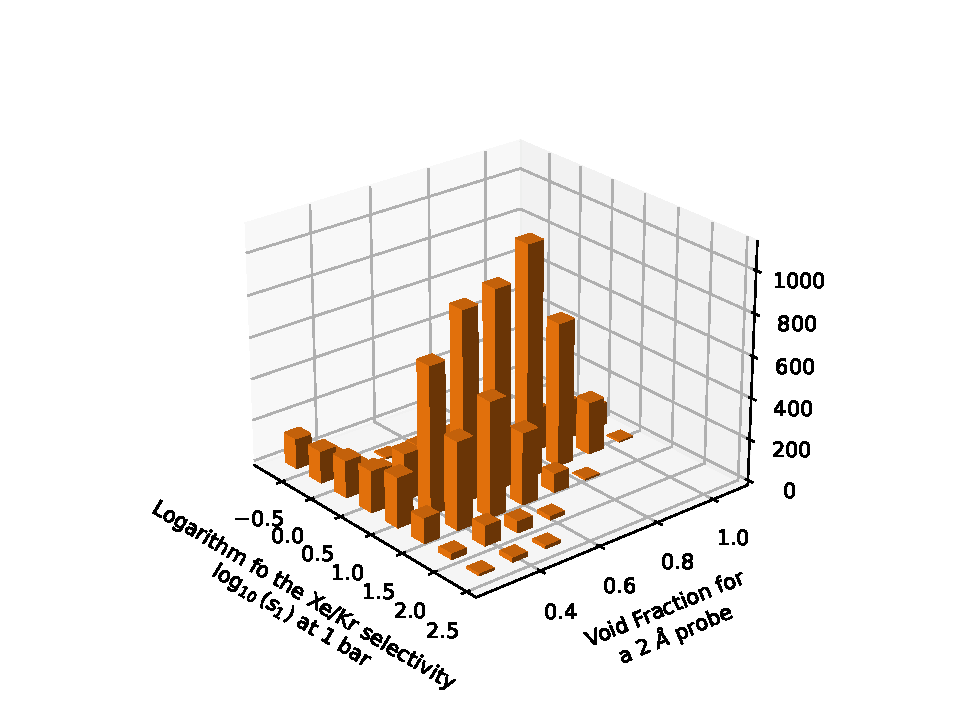
\includegraphics[width=0.48\textwidth,trim={2cm 0 2cm 2cm},clip]{figures/2-thermo/3D_hist_selec_vol.pdf}
  \caption{3D histograms of in a bidimensional space formed by the Xe/Kr selectivity and the surface areas (on the left) and formed by the Xe/Kr selectivity and the pore void fractions (on the right). A base 10 logarithm has been applied to the selectivity values. Bin size increased by 2.4 (on log scale) for the selectivity, by about $500$~\si{\square\meter\cubic\centi\meter} for the surface areas and by $0.125$ for the void fraction. }\label{fgr:3D_hist_sa_vol}
\end{figure}

\subsubsection{Void fraction and selectivity}

A similar analysis for void fraction was also conducted by Wilmer et al.\ for methane storage applications (Figure 5 of Ref.~\cite{Wilmer_2012}) and they found an optimal void fraction value of approximately $0.8$. As shown by the plots in Figure~\ref{fgr:vol}, materials with the highest value of Xe uptake tend to have void fraction values around $0.5$, whereas those with the highest selectivity value exhibit much lower void fractions around $0.1$. The optimal range of void fraction for maximizing uptake lies between $0.2$ and $0.6$, while for selectivity, the optimal range is completely dissociated and falls below $0.2$. Utilizing the void fraction as a descriptor allows for a more refined characterization of selectivity compared to the use of surface area, even though both descriptors yield very similar results. It becomes evident that both descriptors describe a relatively dense material with ``microporosity'', in accordance with the IUPAC definition\autocite{Sing_1985}, indicating materials with medium-low pore volume and surface area.

\begin{figure}[ht]
  \centering
  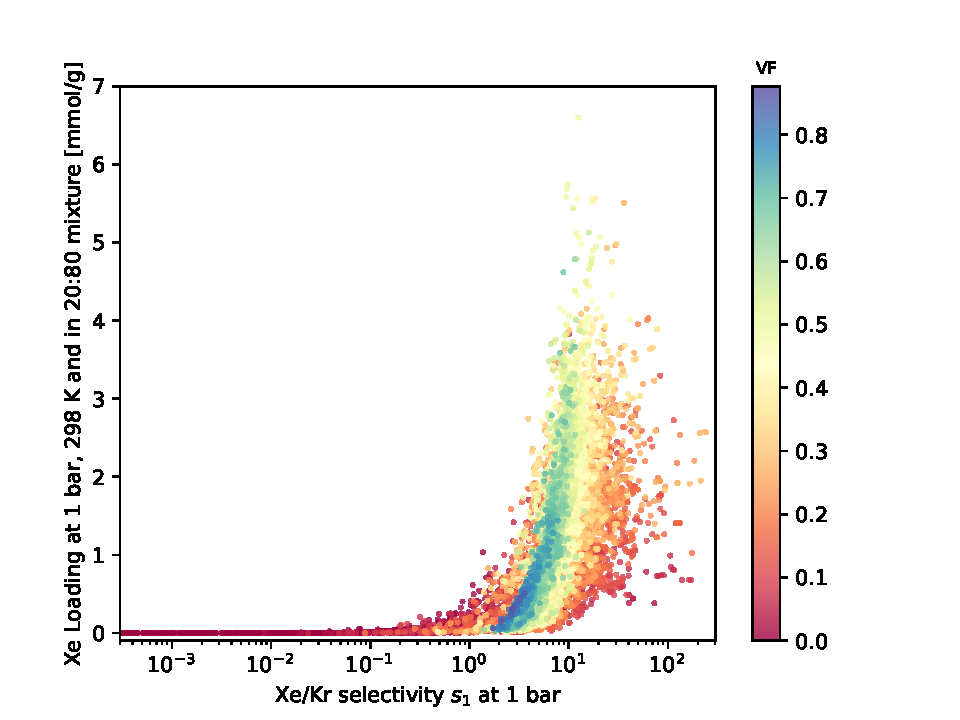
\includegraphics[width=0.48\textwidth]{figures/2-thermo/Scatterplot_uptake_selectivity_vol.pdf}
  \hfill
  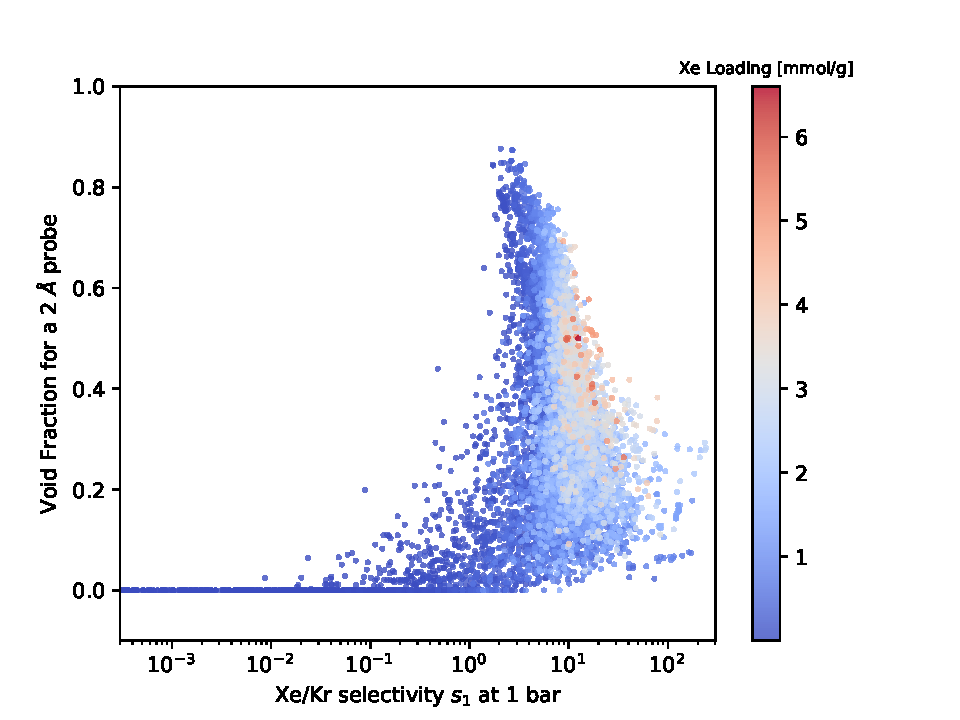
\includegraphics[width=0.48\textwidth]{figures/2-thermo/Scatterplot_vol_selectivity.pdf}
  \caption{On the left: scatterplot of the xenon uptake as a function of the selectivity and labeled by the values of the void fraction. On the right: scatterplot of the selectivity and the void fraction labeled by the quantity of xenon adsorbed. The selectivity and uptake are calculated by a GCMC simulation of a 20:80 Xe/Kr mixture.}\label{fgr:vol}
\end{figure}

By conducting a similar analysis to that performed for surface areas, but this time focusing on the void fraction using Figure~\ref{fgr:3D_hist_sa_vol} (right), it is possible to identify different intervals of void fractions that correspond to highly selective materials. For instance, selectivity values above $92$ correspond to materials with a porosity ranging from {$0$\%} to {$37.5$\%} (with a higher peak between {$12.5$\%} and {$25$\%}). Selectivity values between $92$ and $35$ can be found in materials with a void fraction ranging from {$0$\%} to {$50.0$\%} and more frequently concentrated between {$12.5$\%} and {$37.5$\%}. Selectivity values between $35$ and $13$ can be observed in materials with a void fraction ranging from {$0$\%} to {$75.0$\%}, with a bell-shaped distribution centered around {$31$\%}. As selectivity values decrease, the peak of the distribution shifts towards higher void fraction values, indicating a preference for lower porosity (below {$25$\%}) in terms of selectivity performance. However, similar to surface areas, the void fraction is not a deterministic variable — the void fraction alone does not determine the material's performance. Therefore, it is necessary to investigate whether adding another variable, such as pore size, as a joint variable, can provide a better characterization of the material's performance. As a temporary conclusion, the most selective materials are little porous with a void fraction not exceeding $0.5$ and with an internal surface lower than \SI{2500}{\square\m\per\cubic\cm}. These materials have pores that are specialized for xenon adsorption, which will be confirmed by the following discussion.

\subsubsection{Pore Size and selectivity}

The optimal pore size for xenon/krypton separation can be deduced from Figure~\ref{fgr:lcd}. As shown on the right plot, the most selective materials have a pore size close to \SI{5}{\angstrom}. However, it is challenging to distinguish between materials with very low selectivity that have a similar label color. To better visualize the differences, different colors were used to represent structures with D$_i$ values ranging from $3.6$ to $11.6$~\si{\angstrom}. It becomes evident that the pore size should be around \SI{5}{\angstrom}, but if it is too small (near \SI{4.5}{\angstrom}),the selectivity significantly decreases. Therefore, there exists a sweet spot of pore size values that enable the attainment of very high selectivity.

\begin{figure}[ht!]
  \centering
  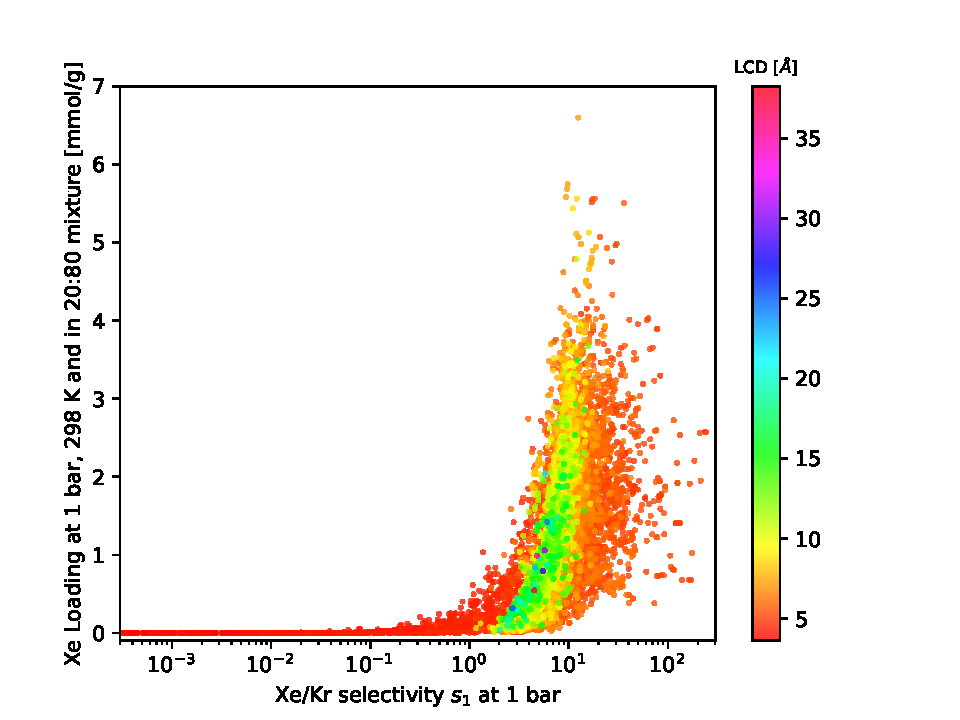
\includegraphics[width=0.48\textwidth]{figures/2-thermo/Scatterplot_uptake_selectivity_lcd.pdf}
  \hfill
  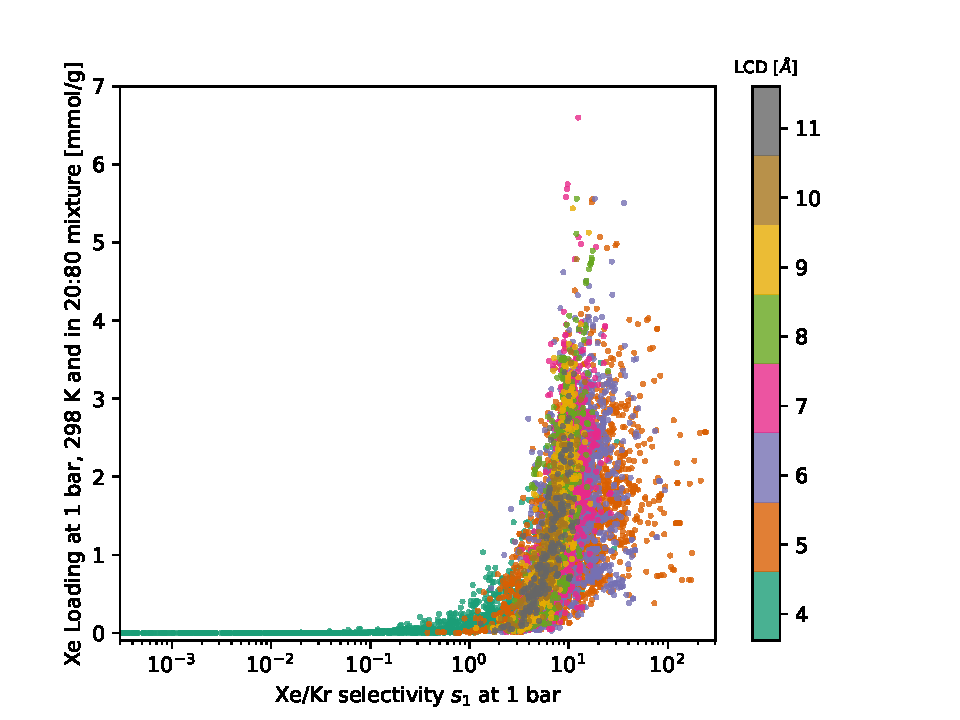
\includegraphics[width=0.48\textwidth]{figures/2-thermo/Scatterplot_uptake_selectivity_lcd_zoom.pdf}
  \caption{Scatterplot of the xenon uptake as a function of the selectivity (20:80) and labeled by the values of LCD\e{UFF} (left). The same scatterplot restricted to values of D$_i$ between ($3.6$ and $11.6$~\si{\angstrom}) and labeled using a different color code to distinguish the most selective materials from the least selective ones. The most selective materials are colored in orange corresponding to a pore size adapted for xenon adsorption (around $5$~\si{\angstrom}). The least selective ones are in green, with a pore lower than the size of a xenon hence preventing its adsorption.}\label{fgr:lcd}
\end{figure}

The joint effects of void fraction and largest cavity diameter (D$_i$) on selectivity reveal a distinct region in the bidimensional descriptor space where the most selective materials are located. On Figure~\ref{fgr:lcd_vf}, structures with a selectivity above $10$ are highly likely to have a void fraction below $0.4$ with a relatively wider range of D$_i$. However, as shown on the filtered version of the plot (on the right), the most selective materials (over $40$) exist within a very narrow range of D$_i$ values, approximately between $4.8$ and $6$~\si{\angstrom}. This can be attributed to the xenon atom size, which closely matches these D$_i$ values, which allows a maximal stabilization of xenon. On the other hand, krypton, being slightly smaller, exhibits less favorable interaction with the pores, resulting in higher observed selectivity. 

\begin{figure}[ht!]
  \centering
  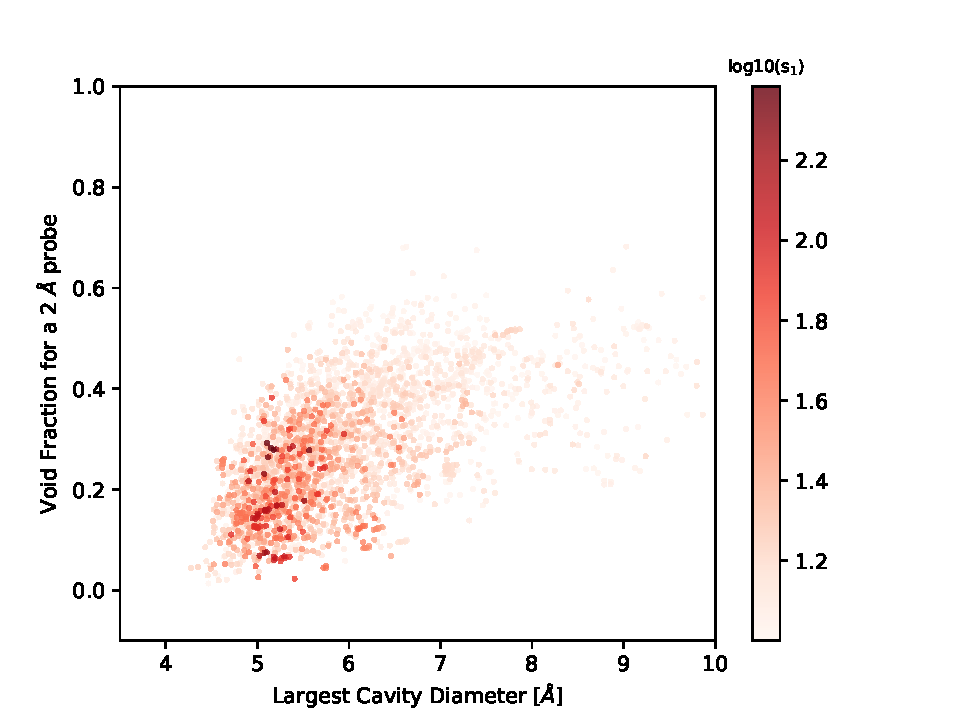
\includegraphics[width=0.48\textwidth]{figures/2-thermo/Scatterplot_vf_lcd_selectivity.pdf}
  \hfill
  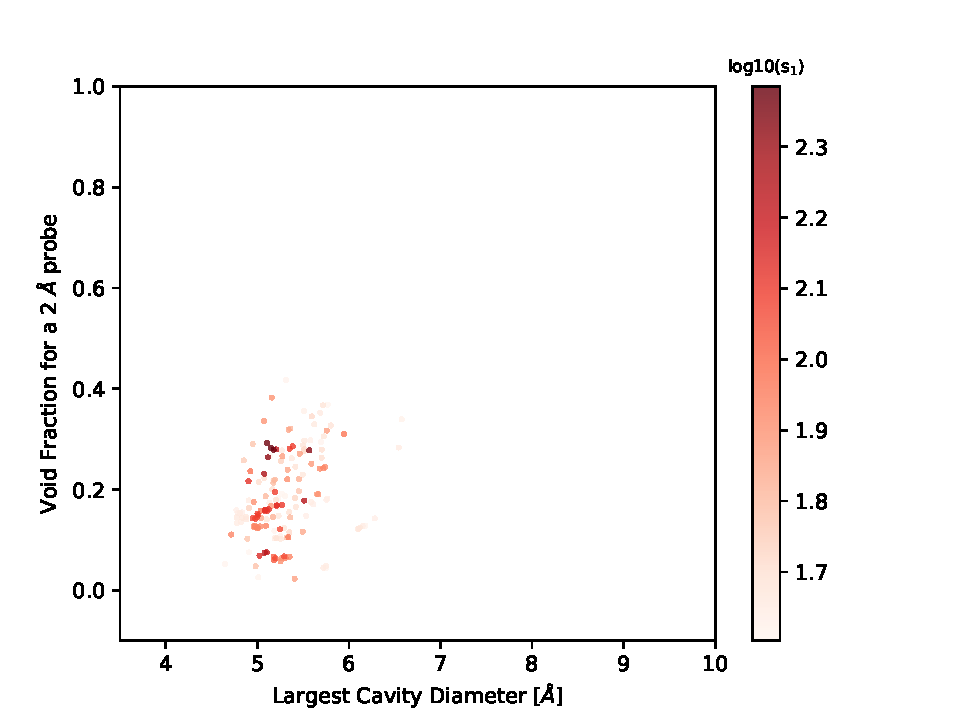
\includegraphics[width=0.48\textwidth]{figures/2-thermo/Scatterplot_vf_lcd_selectivity_zoom.pdf}  
  \caption{Scatterplots of the void fraction as a function of the LCD\e{UFF} and labeled by the log$_{10}$ of the selectivity values. On the left, only the materials with a selectivity between $10$ and $40$ are considered; and on the right, selectivity values over $40$.}\label{fgr:lcd_vf}
\end{figure}


As presented in Chapter 1, Simon et al.\ found that the most selective materials have a pseudo-spherical shape with a size close to the diameter of a xenon. These materials tend to have a dense structure with limited porosity. In this slightly different approach specific intervals of cavity diameter and pore volume have been associated with high selectivity, thus confirming the size requirement already identified by other studies. However, this structure--property relationship serves as a description tool for identifying selective materials, and it does not enable accurate predictions based solely on structural descriptors. 

\subsubsection{Effect of the composition}

The previous analyses focused on a specific type of mixture composition (20:80) associated with the extraction of xenon and krypton from air through cryogenic distillation (see section~\ref{sct:industrial}). In the following section, the effects of composition will be investigated by considering the case of xenon/krypton separation in spent nuclear fuel off-gases. In nuclear applications, the mixture has a higher xenon content than in the previous one, with a typical 90:10 Xe/Kr ratio. For this reason, the quantity of xenon adsorbed in the materials will mechanically be higher compared to the previous scenario. However, the second quotient in the formula of selectivity in equation~\ref{eq:selec} compensates for the inherently higher first quotient. The objective of this analysis is to evaluate these two effects and determine whether they offset each other or if different trends emerge depending on the composition value. 

As depicted in Figure~\ref{fgr:SI:overview_2080_9010}, the selectivity values of both compositions are relatively similar. However, a slight decrease in performance can be observed when increasing the proportion of xenon in the mixture, particularly for materials with moderate selectivity ($s$ between $2$ and $50$). This decline in performance can be attributed to variations pores displayed by the material, which possess different affinities for xenon. When the xenon proportion is lower, Xe adsorbates preferentially access the most favorable pores, resulting in a concentration of the small quantity xenon in these sites. However, as the xenon content increases, these most favorable sites become saturated, and xenon needs to compete with krypton for less favorable sites, thereby slightly decreasing the selectivity.

\begin{figure*}[ht]
  \centering
    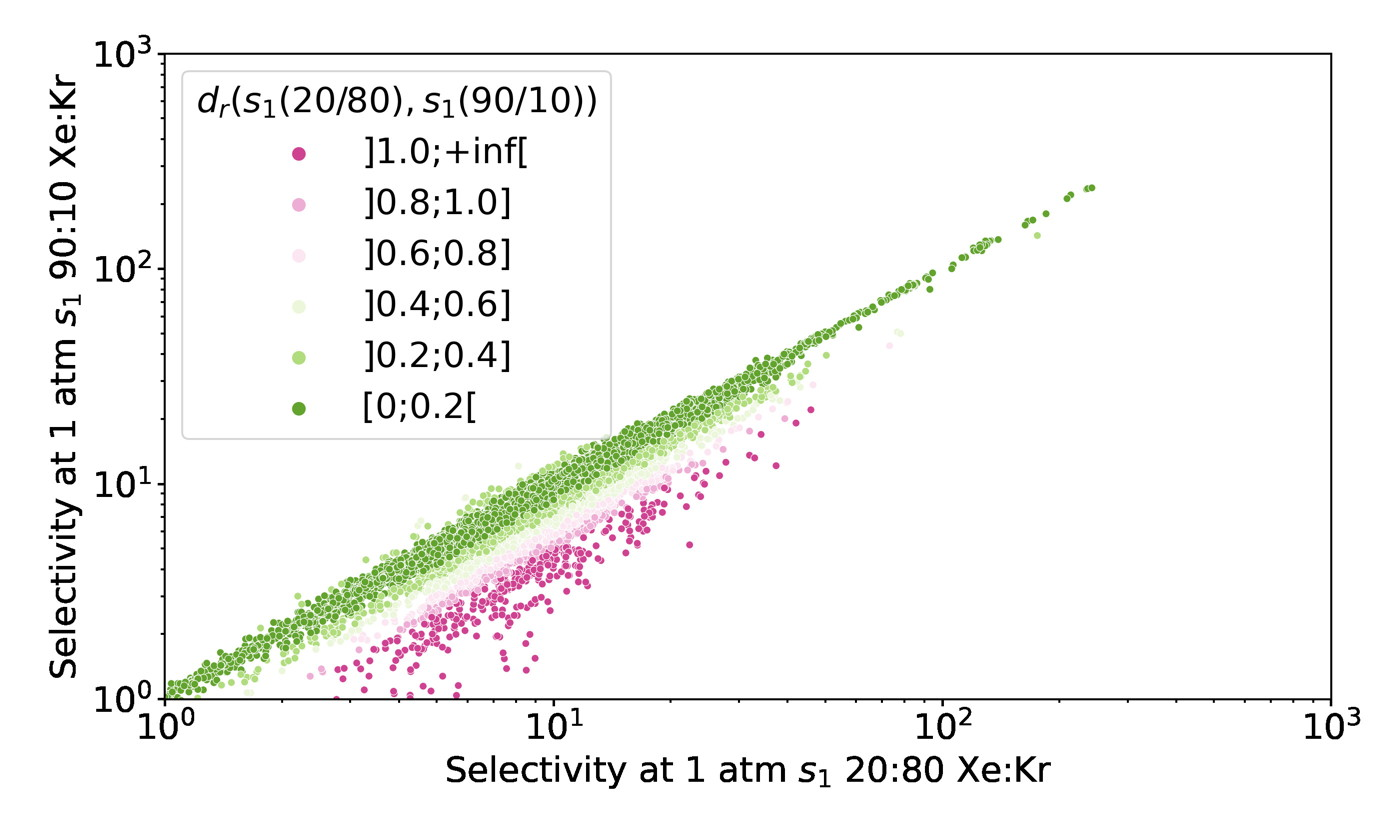
\includegraphics[width=0.45\textwidth]{figures/2-thermo/s_2080_vs_s_9010_overview_log.jpg}
    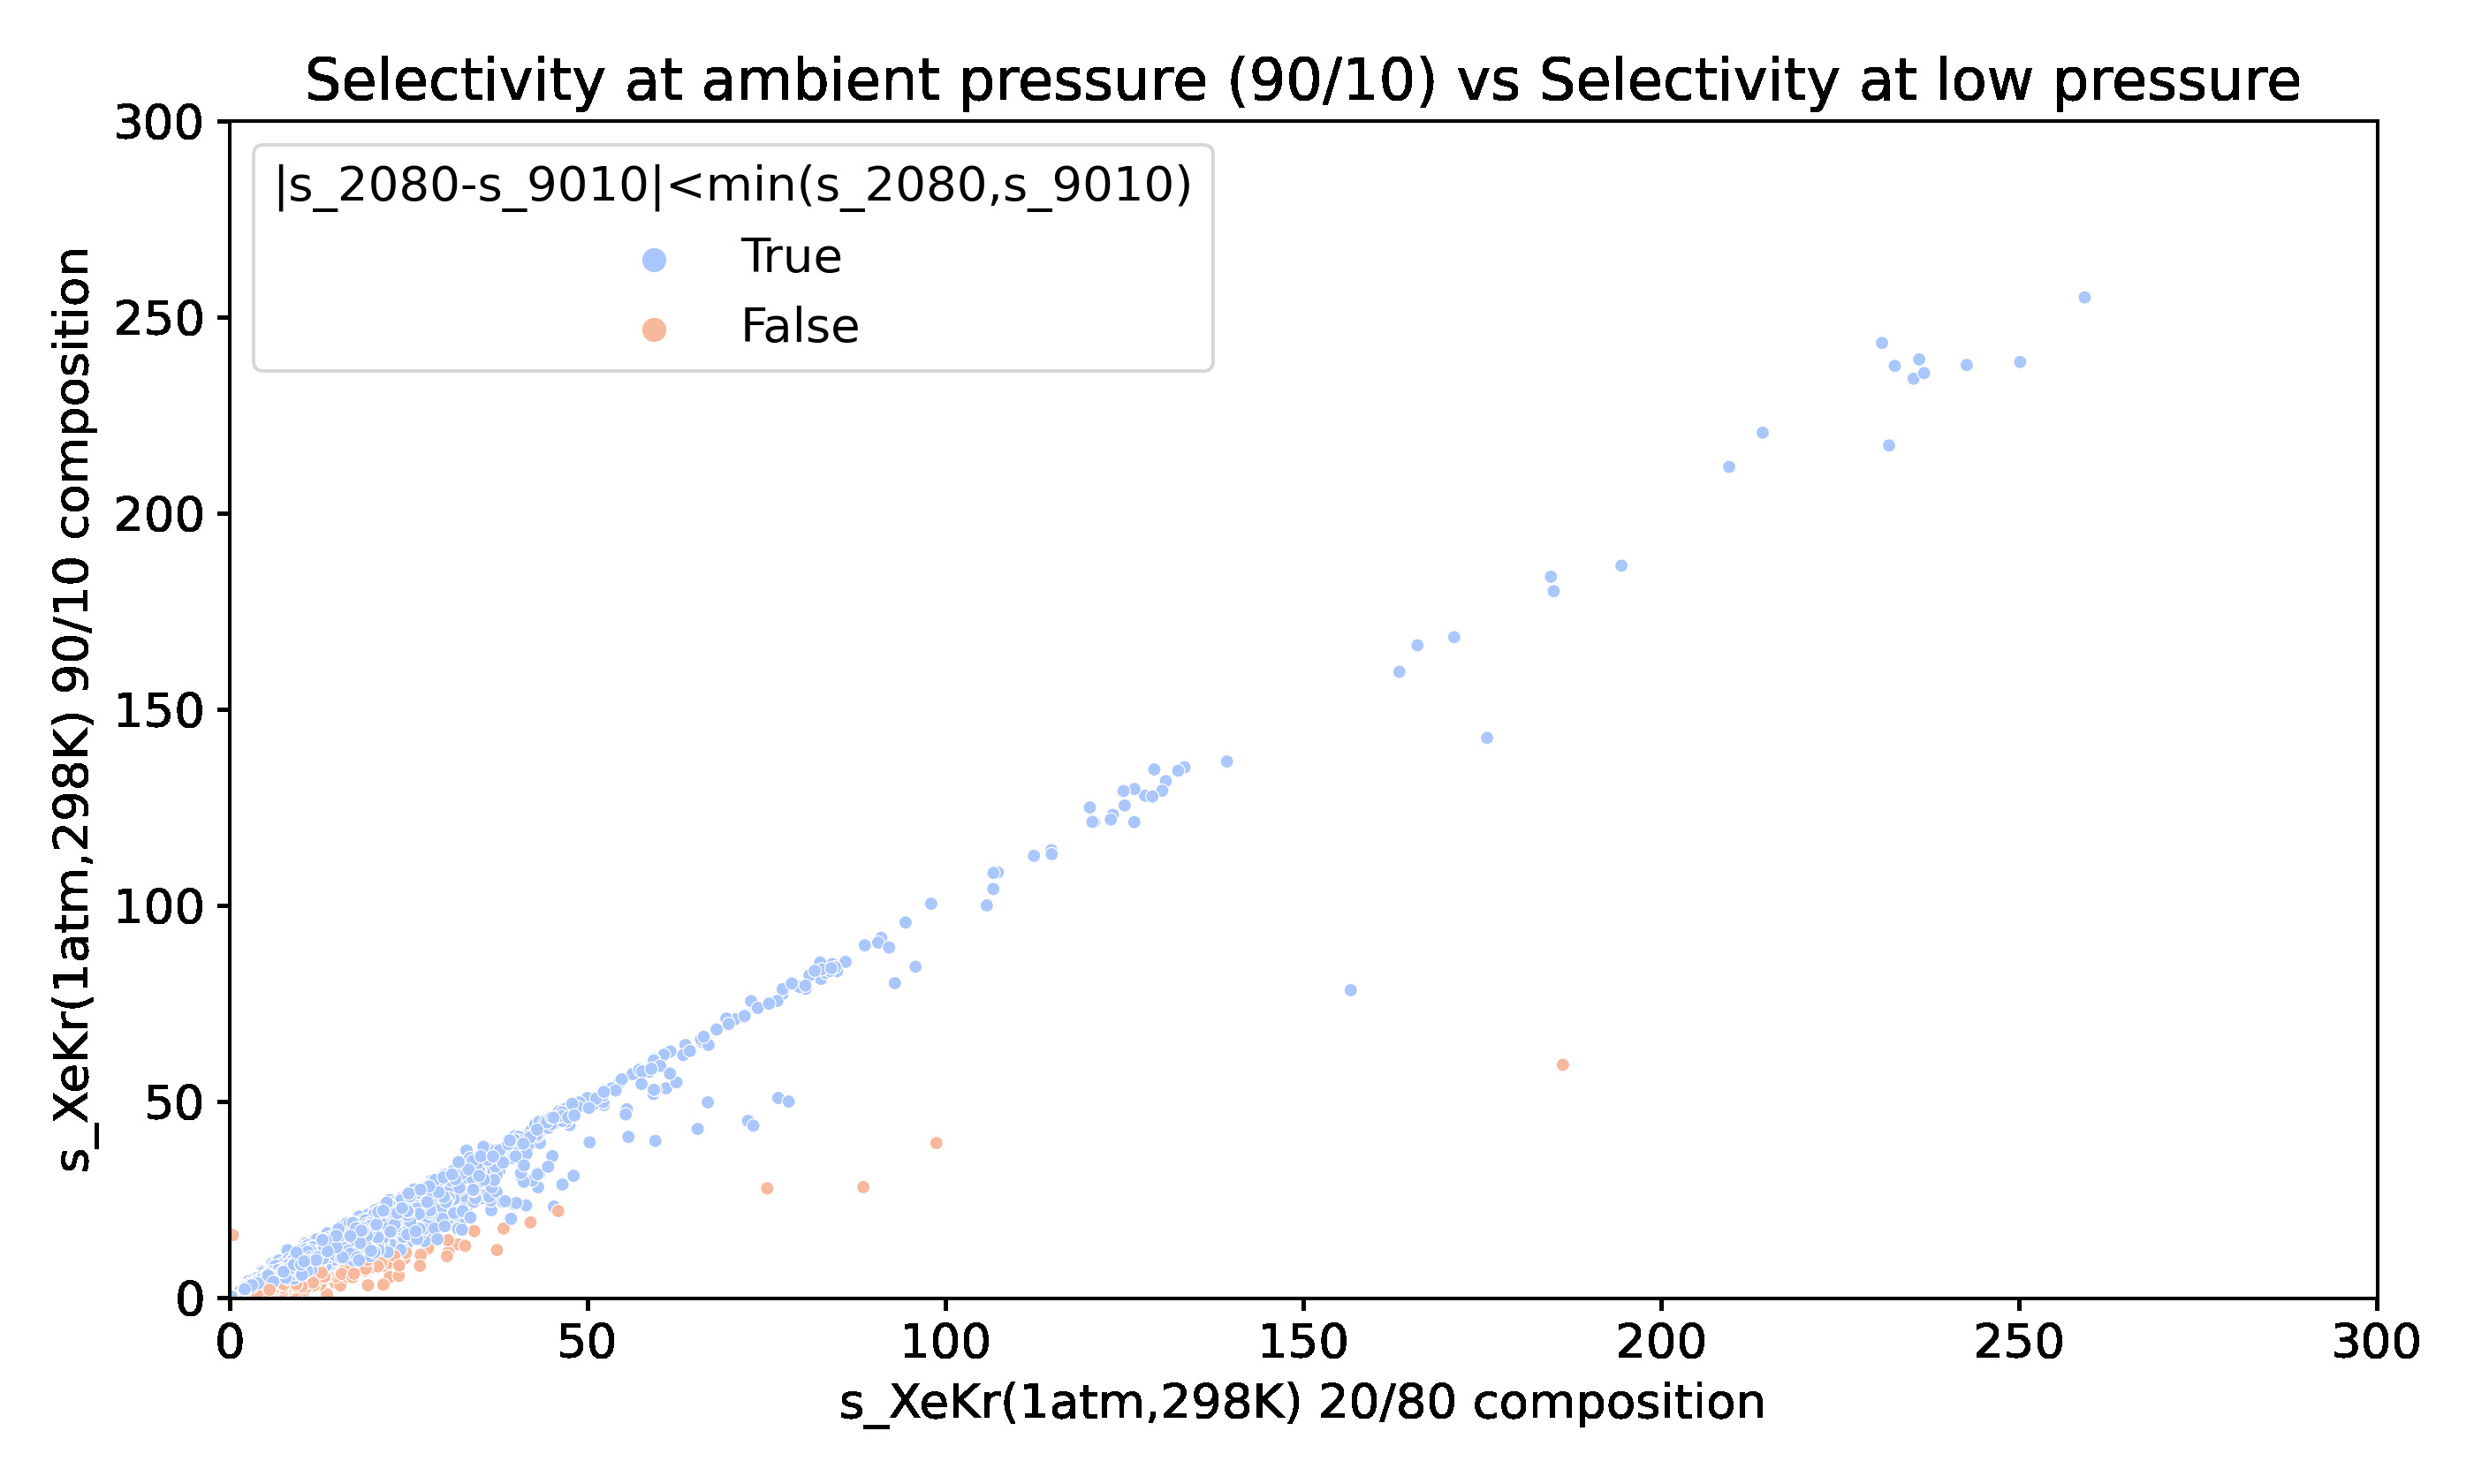
\includegraphics[width=0.45\textwidth]{figures/2-thermo/s_2080_vs_s_9010_overview.jpg}
    \caption{Illustration (scatterplot) of the difference of selectivity ($s\e{1}(20:80)$ and $s\e{1}(90:10)$) for two different Xe/Kr mixture compositions 20:80 (x-axis) and 90:10 (y-axis) at \SI{1}{\atm} and \SI{298}{\kelvin}. On the left, the axis is in log scale and the relative difference of selectivity between the two compositions is particularly high for the points labeled in purple. On the right, the axis is in linear scale and the points are labeled only to differentiate the materials with relative difference under and over $1$.}\label{fgr:SI:overview_2080_9010}
  \end{figure*}

%higher uptakes
The effect of the composition on the different analyses of the different structural descriptors will be discussed here. Notably, when considering a mixture with a higher xenon content, the xenon uptake values experience significant change. The nanopores of selective materials ($1<s_1\leq 50$) are much more saturated with Xe, resulting in a substantially higher maximum xenon uptake. Comparing the Figures~\ref{fgr:vol} and~\ref{fgr:compo}, the maximum uptake increases from \SI{6.6}{\milli\mole\per\gram} (for the 20:80 composition) to \SI{11.7}{\milli\mole\per\gram}. In the case of moderately selective materials at the 20:80 composition, the xenon competes with krypton primarily in the most selective nanopores. However, with a higher xenon content, xenon has to compete with krypton in much less favorable sites due to saturation of the most preferable sites. It is worth noting the previous conclusion regarding the maximum uptake of xenon for the most selective materials ($s_1>50$) remains valid. The maximum xenon uptake reaches up to \SI{4.0}{\milli\mole\per\gram}, and it increases slightly to \SI{4.2}{\milli\mole\per\gram} for the composition with a higher xenon content. Despite the change in composition, the nature of the adsorbed state remains unchanged due to the extremely high selectivity, resulting in similar quantities of xenon being present in the pores. Consequently, the higher xenon content does not significantly influence the performance of the most selective materials, but it can alter selectivity and greatly increase the xenon uptake for some moderately selective materials.

\begin{figure}[ht!]
  \centering
  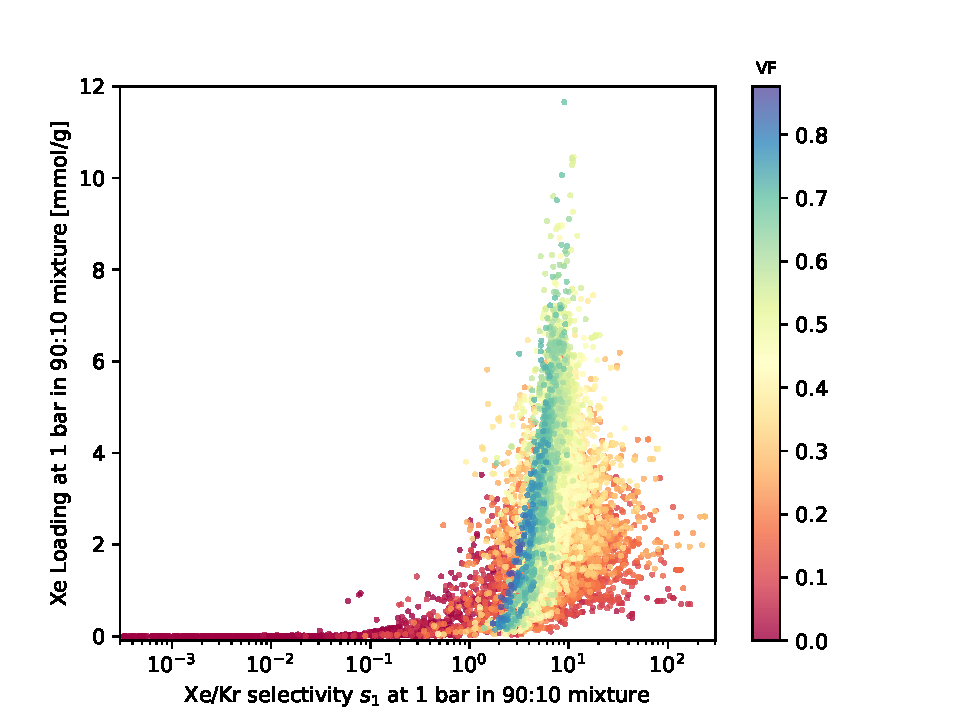
\includegraphics[width=0.48\textwidth]{figures/2-thermo/Scatterplot_uptake_selectivity_vol_9010.pdf} 
  \hfill 
  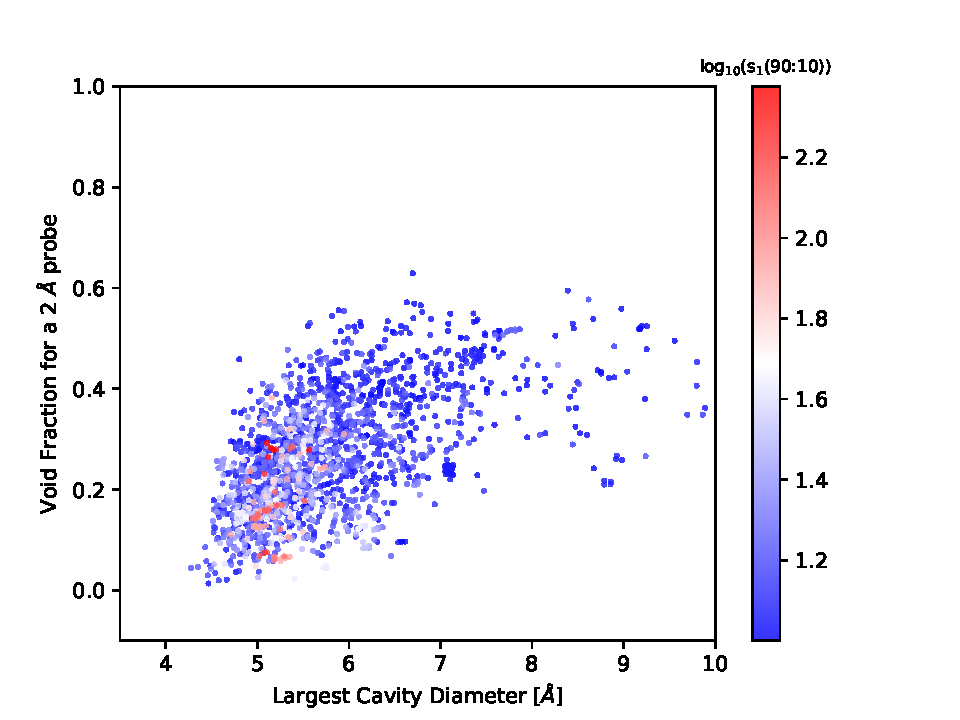
\includegraphics[width=0.48\textwidth]{figures/2-thermo/Scatterplot_vf_lcd_selectivity9010.pdf}
  \caption{Illustration of the effect of the composition by representing the same figures as in~\ref{fgr:vol} and~\ref{fgr:lcd_vf} but for a 90:10 composition. On the left: scatterplot of the xenon uptake as a function of the selectivity ($s\e{1}(90:10)$) and labeled by the values of the void fraction. On the right: scatterplots of the void fraction as a function of the LCD\e{UFF} and labeled by the selectivity ($s\e{1}(90:10)$) values superior to $10$ in log-scale.}\label{fgr:compo}
\end{figure}

As a conclusion, the composition does not seem to affect the previously determined structural characteristics required for high selectivity. As depicted in the right plot of the Figure~\ref{fgr:compo} (right), the most selective materials still exhibit a pore size of approximately \SI{5}{\angstrom} and a porosity below {$40$\%}. This structural domain serves as necessary conditions for achieving selectivity, but they are not sufficient as less selective materials can also display these characteristics. Having established the geometric conditions necessary for obtaining good selectivity, the focus now shifts towards understanding the thermodynamic origins of selectivity by examining energy-based quantities and the various correlations among them.

\subsection{Thermodynamic quantities correlations at infinite dilution}

In this section, my goal is to map out the details of the thermodynamic features of Xe/Kr adsorption and separation in nanoporous materials, rather than to directly address the structure--property relationships. The high-throughput screening methodology was used to map out the space of thermodynamic properties, surpassing the conventional metrics of selectivity and uptake. The specific emphasis was placed on investigating the role of adsorption enthalpy and entropy, differentiating between Xe and Kr adsorption thermodynamics, and analyzing the variations in selectivity at both low and high pressures. The discussion below is based on a work published\footnote[1]{The related data can be found at \url{https://github.com/fxcoudert/citable-data/tree/master/132-Ren_FaradayDiscuss_2021}} in the Faraday Discussions Ref.~\cite{Ren_2021}.

To assess the performance of a given nanoporous material for separation in the low loading (or low pressure) limit, Henry constants are commonly calculated by linearly fitting low-pressure adsorption isotherm data --- both experimentally and computationally. In this section, the thermodynamics of Xe and Kr adsorption at low pressure are investigated. Specifically, the low-pressure adsorption properties are obtained using the Widom insertion method\autocite{Widom1963, frenkel2001widom} on a dataset of 9\,668 selected structures. This method provides higher accuracy compared to fitting isotherms, where it can be challenging to determine the extent of the linear adsorption regime. Through these simulations, Henry constants $K$ and adsorption enthalpies $\Delta\e{ads}H\e{0}$ (at the zero loading limit) are calculated for both xenon and krypton. The Xe/Kr thermodynamic selectivity $s\e{0}$ in the low-pressure limit is then determined by the ratio $s\e{0} = K\ex{Xe}/K\ex{Kr}$ of the Henry constants for the two gases. In the following discussion, the statistical relationships among the thermodynamic quantities at low pressure, namely $s\e{0}$, $K\ex{Xe}$, $K\ex{Kr}$, $\Delta\e{ads}H\e{0}\ex{Xe}$, $\Delta\e{ads}H\e{0}\ex{Kr}$ and $\Delta\e{exc}H\e{0}$, will be examined.

\begin{figure}[h]
  \centering
    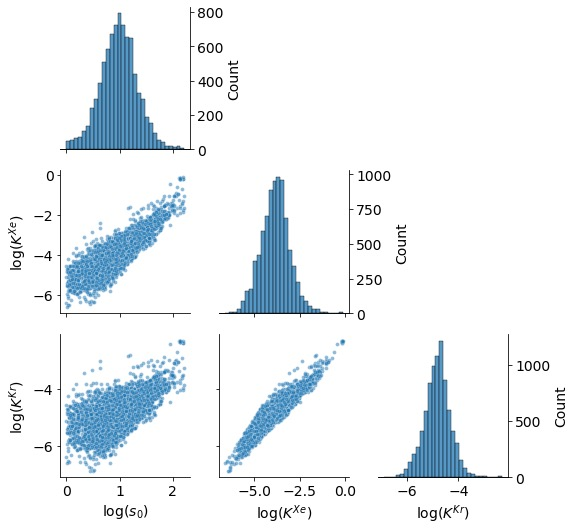
\includegraphics[width=0.45\textwidth]{figures/2-thermo/Henry_0.jpg}
    \caption{For 8\,401 MOFs with favorable thermodynamic Xe/Kr selectivity ($s\e{0} > 1$), pair plots of $\log\e{10}(s\e{0})$, $\log\e{10}(K\ex{Xe})$ and $\log\e{10}(K\ex{Kr})$ (the Henry constants are in~\si{\milli\mol\per\gram\per\pascal}) in the off-diagonal subplots (note that the y-axis is displayed on the right side) and the distribution of each quantity are on the diagonal (note that the y-axis displayed on the right side corresponds to the count and the x-axis is correctly labeled below each subplot).}\label{fgr:histo_K}
  \end{figure}
  
The distribution of thermodynamic properties of materials with favorable thermodynamic Xe/Kr selectivity ($s\e{0} > 1$) is depicted in Figure~\ref{fgr:histo_K}. It is important to note that the plots focus on selectivity values above 1, as these are the materials of interest for separation. This selection eliminates certain outliers with specific geometries or binding sites (without significantly altering the overall conclusions). The plots reveal that while the logarithm of Xe Henry constant $K\ex{Xe}$ exhibits a weak correlation with the logarithm of selectivity $s\e{0}$, this correlation is stronger for highly selective materials. Therefore, in a multistep screening study aimed at identifying the most selective materials, it could be possible to utilize as a ``first filter'' criterion based purely on Xe adsorption, by excluding materials below a certain threshold (e.g., the materials with $s_0\ge30$ can be found in the subset with $K\ex{Xe}\ge2.7\,10^{-1}$~\si{\milli\mol\per\gram\per\pascal}). On the other hand, the correlation between $K\ex{Kr}$ and $s\e{0}$ is relatively weaker. These results suggest that a high affinity with xenon measured by the Henry constant is a determining factor of high selectivity for the most selective materials.  

\begin{figure}[h]
  \centering
    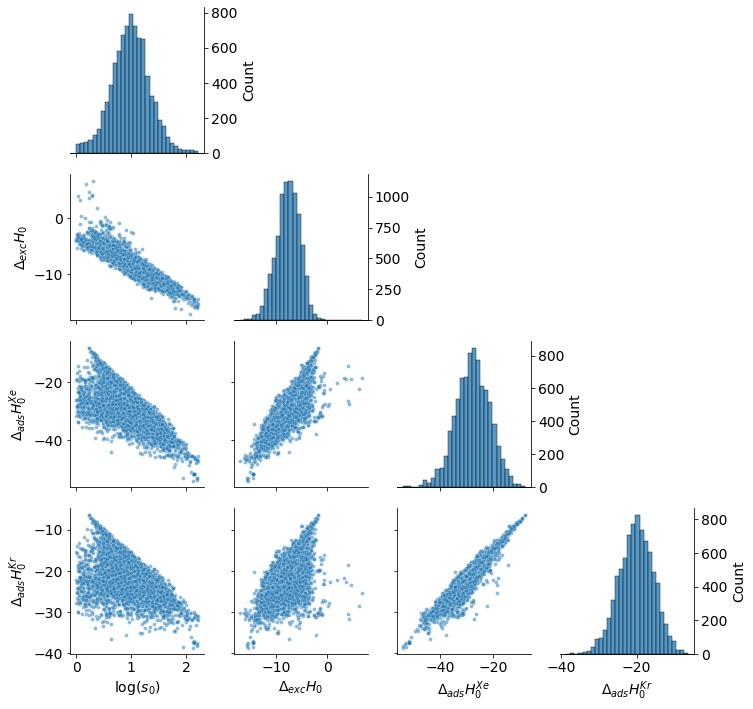
\includegraphics[width=0.6\textwidth]{figures/2-thermo/Enthalpy_0_log.jpg}
    \caption{For 8\,401 MOFs with favorable thermodynamic Xe/Kr selectivity ($s\e{0} > 1$), pair plots of $\log(s\e{0})$, $\Delta\e{exc}H\e{0}$, $\Delta\e{ads}H\ex{Xe}\e{0}$ and $\Delta\e{ads}H\ex{Kr}\e{0}$ (the enthalpies are in~\si{\kilo\joule\per\mol}) in the off-diagonal subplots and the distribution of each quantity is on the diagonal.}\label{fgr:histo_H}
  \end{figure}

In terms of Henry constants, a diverse range of behaviors is observed, with $K\ex{Xe}$ ranging from $2.6\,10^{-7}$ to $7.9\,10^{-1}$~\si{\milli\mole\per\gram\per\pascal}, and $K\ex{Kr}$ ranging from $1.3\,10^{-7}$ to $5.1\,10^{-3}$~\si{\milli\mole\per\gram\per\pascal}.  Additionally, there is a statistical trend indicating that a high affinity for xenon typically translates into a relatively high affinity for krypton. This general trend is observed for noble gases, where the adsorption sites lack strong specificity. To delve deeper into the thermodynamic aspects underlying this wide diversity in behavior, the enthalpies involved were plotted in Figure~\ref{fgr:histo_H}.

The low-loading adsorption enthalpy of xenon ($\Delta\e{ads}H\ex{Xe}\e{0}$) is strongly correlated with that of krypton ($\Delta\e{ads}H\ex{Kr}\e{0}$), which aligns with the correlation observed between their respective Henry constants. This suggests the involvement of a rather generic physisorption mechanism in the majority of materials, where the host--adsorbate affinities are primarily determined by the enthalpy. The selectivity of Xe/Kr selectivity is not driven significantly by the xenon or krypton adsorption enthalpy alone (both exhibit weak correlation with selectivity), but rather by their difference, $\Delta\e{exc}H\e{0}$, which shows a strong correlation with $\log(s\e{0})$. This finding is further supported by the lack of correlation between selectivity and adsorption entropies (\emph{cf.} Figure~\ref{fgr:SI:HS_0_log}), indicating that the separation is predominantly enthalpic in nature, and any dispersion in the correlation between selectivity $\log(s\e{0})$ and $\Delta\e{exc}H\e{0}$ is influenced by entropy.

\begin{figure*}[h]
  \centering
    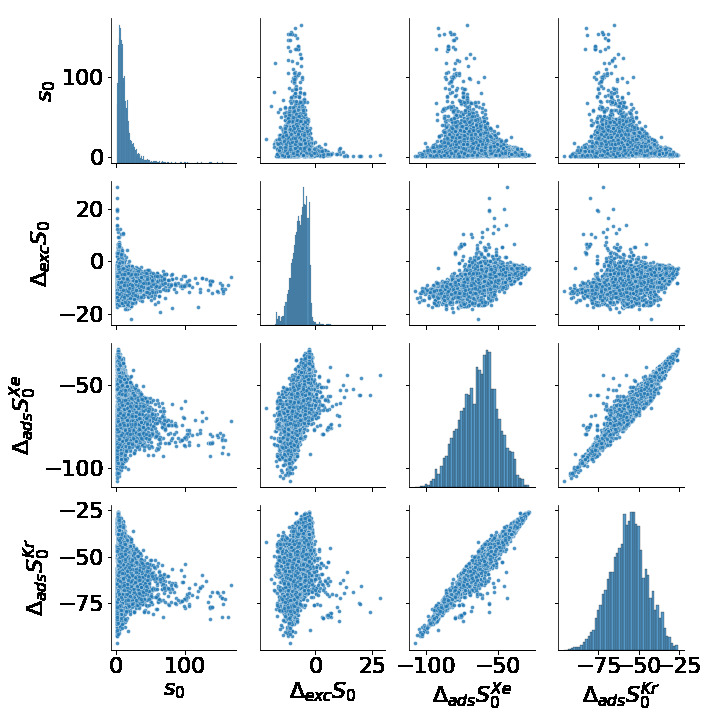
\includegraphics[width=0.45\textwidth]{figures/2-thermo/Entropy_0.jpg}
    \caption{For 8\,401 MOFs with favorable thermodynamic Xe/Kr selectivity ($s\e{0} > 1$), pair plots of $s\e{0}$, $\Delta\e{exc}S\e{0}$, $\Delta\e{ads}S\ex{Xe}\e{0}$ and $\Delta\e{ads}S\ex{Kr}\e{0}$ in the off-diagonal subplots and the distribution of each quantity are on the diagonal.}\label{fgr:SI:HS_0_log}
\end{figure*}

Upon closer analysis of the Figure~\ref{fgr:SI:HS_0_log}, it is observed that the adsorption entropy of xenon and krypton shows a noticeable correlation. However, their difference (the exchange entropy), which represents the exchange entropy, does not exhibit a significant variance value (Figure~\ref{fgr:SI:dist0}) compared to the enthalpy. This suggests that the thermodynamic quantity plays a minor role in the selectivity performance of the materials. However, it is noted that although the most selective materials do not have any exchange entropy values, they are centered around a value of approximately \SI{-10}{\kilo\joule\per\mole\per\kelvin}. While this correlation is not straightforward, it indicates that possessing an exchange entropy within this range is a necessary attribute for achieving selectivity in materials.

\begin{figure*}[ht]
  \centering
    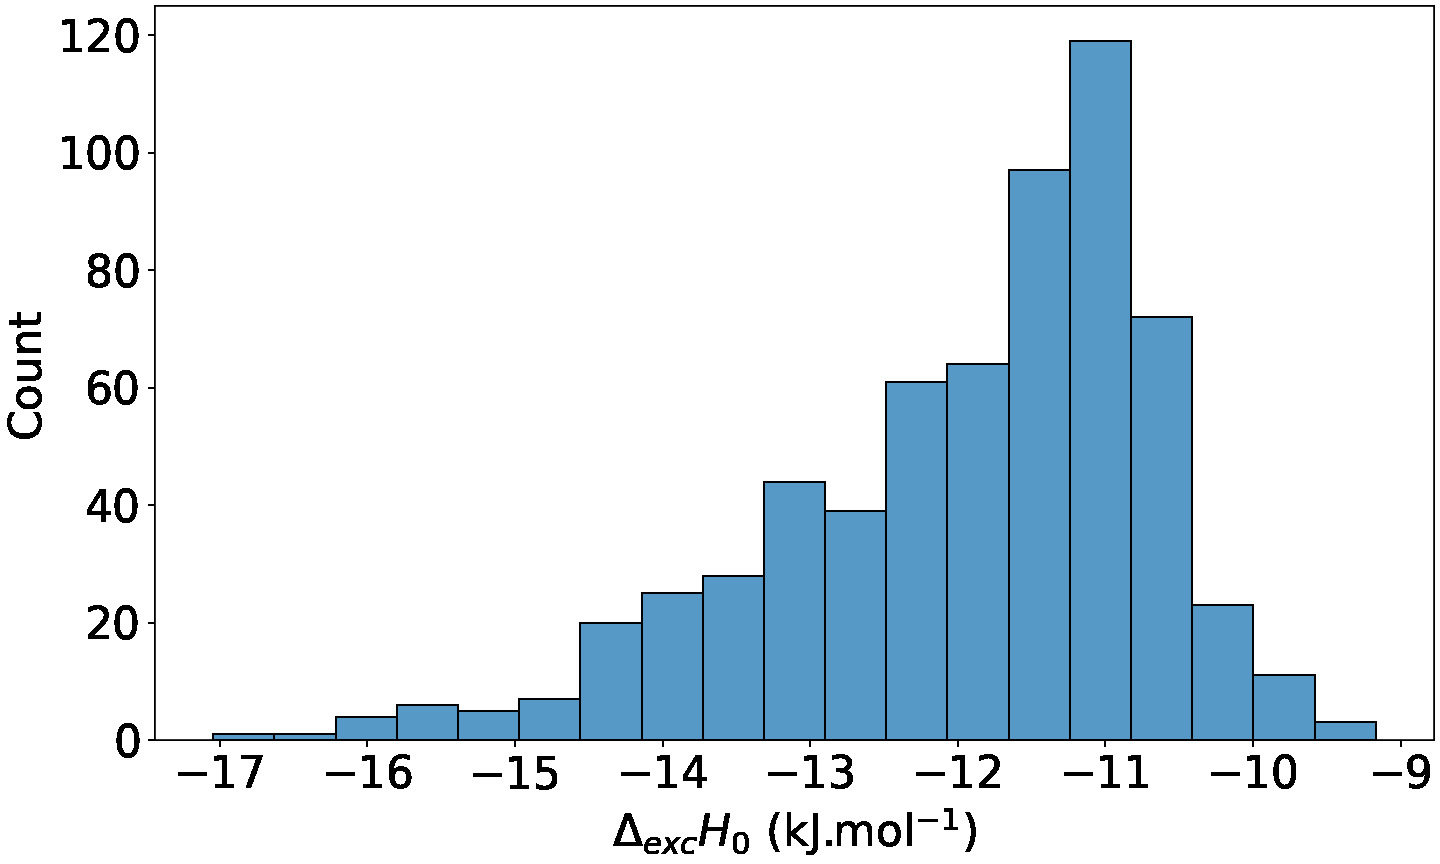
\includegraphics[width=0.45\textwidth]{figures/2-thermo/Delta_H_0.jpg}
    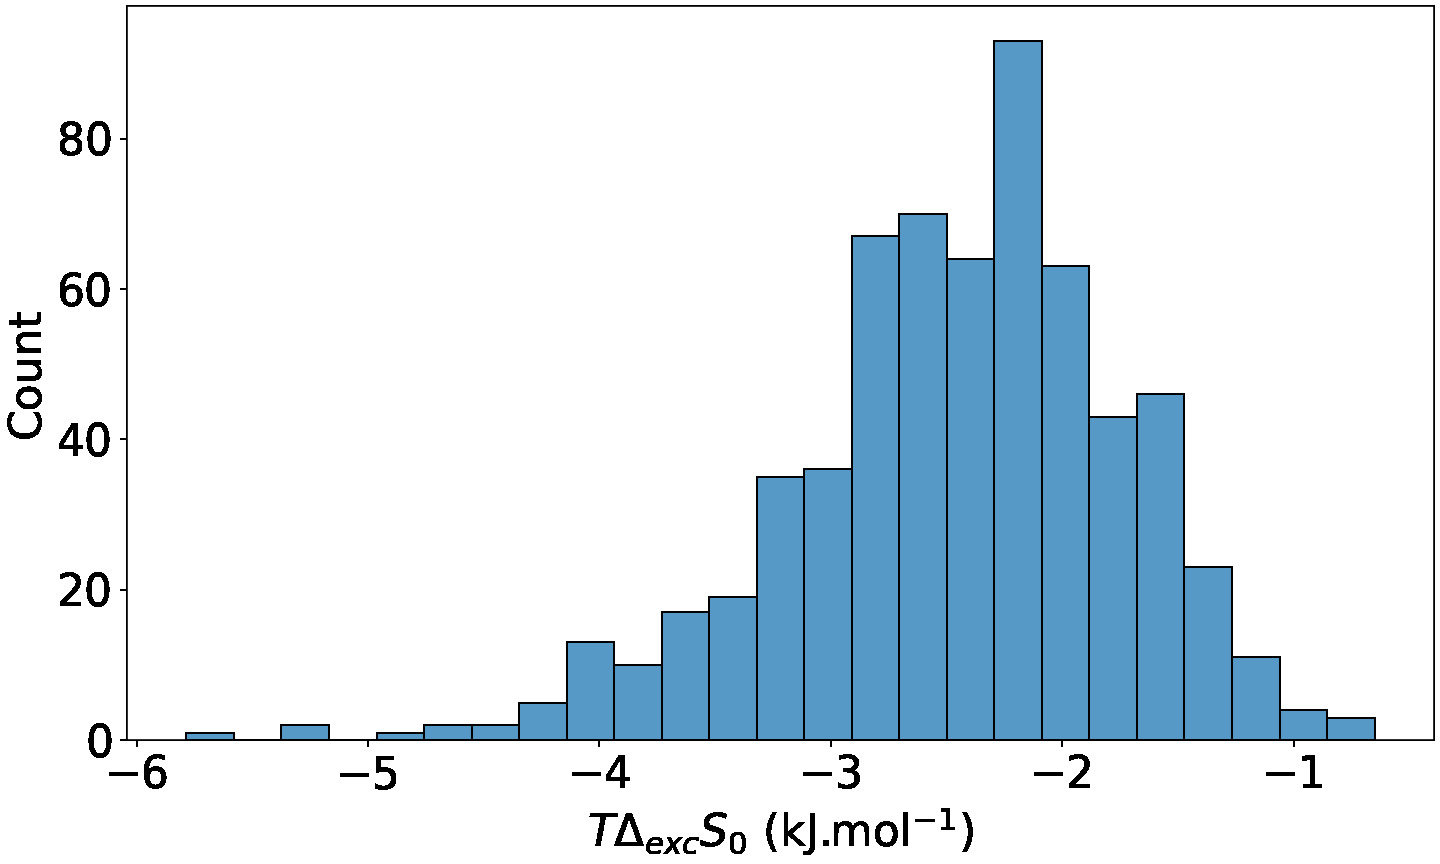
\includegraphics[width=0.45\textwidth]{figures/2-thermo/T_Delta_S_0.jpg}
    \caption{Distribution of the enthalpy $\Delta\e{exc}H\e{0}$ and entropy $T\Delta\e{exc}S\e{0}$ of exchange at low pressure on the 630 most selective structures}\label{fgr:SI:dist0}
\end{figure*}

To further emphasize the enthalpic nature of the separation process, the base-10 logarithm of the Henry constant (proportional to the adsorption free energy) is compared to the adsorption enthalpy for both xenon and krypton. As shown in Figure~\ref{fgr:SI:HK}, the free energy can be predominantly explained by the enthalpy, which confirms the secondary role played by entropy in accounting for the dispersion in this relationship. The effect of entropy weakens the correlation for materials with less favorable adsorption, but as the adsorption enthalpies become increasingly negative, the correlation becomes increasingly stronger. The most selective materials have an almost negligible entropic contribution to the final free energy value ($G=H-TS$).

\begin{figure*}[ht]
  \centering
    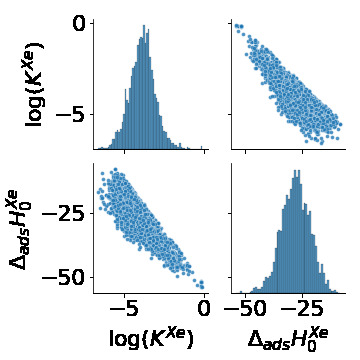
\includegraphics[width=0.35\textwidth]{figures/2-thermo/H_K_Xe.jpg}
    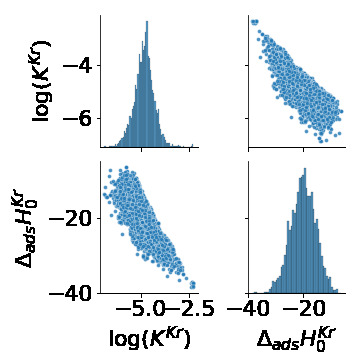
\includegraphics[width=0.35\textwidth]{figures/2-thermo/H_K_Kr.jpg}
    \caption{For 8\,401 MOFs with favorable thermodynamic Xe/Kr selectivity ($s\e{0} > 1$), pair plots of $\log(K\e{H}\ex{i})$ and $\Delta\e{ads}H\ex{i}\e{0}$ in the off-diagonal subplots for both i$=$Xe and i$=$Kr and the distribution of each quantity are on the diagonal.}\label{fgr:SI:HK}
\end{figure*}

Upon further analysis of Figure~\ref{fgr:henry_enthalpy}, it becomes apparent that the entropic effect is influenced by the pore size. Specifically, larger pore sizes tend to yield more positive entropic terms (the entropic term refers to $-T\Delta\e{ads}S$). This observation elucidates the weaker correlation observed for less attractive materials throughout the pairplot of Figures~\ref{fgr:histo_H} and~\ref{fgr:histo_K}.

\begin{figure}[ht]
  \centering
  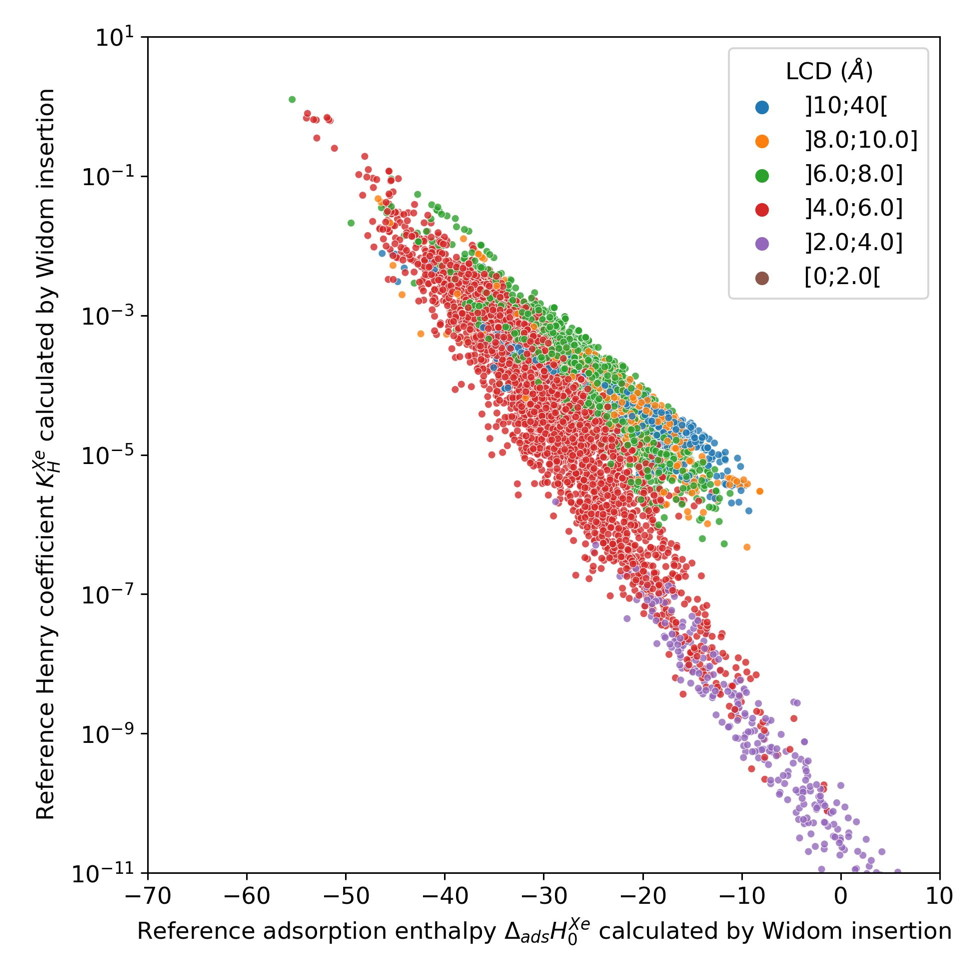
\includegraphics[width=0.4\textwidth]{figures/2-thermo/H_Xe_widom_vs_K_Xe_widom_overview.jpg}
  \caption{Comparison between the Xe Henry constant and Xe adsorption enthalpy labeled by categories of LCD\e{UFF} values for the CoRE MOF structures.}\label{fgr:henry_enthalpy}
\end{figure}

In the analysis of the influence of the pore size and void fraction on the entropic term $T\Delta\e{ads}S\ex{Xe}\e{0}$ (Figure~\ref{fgr:entropy_geometry}), a clear relationship between entropy and pore size, represented by the LCD\e{UFF}\footnote[1]{This corresponds to the diameter of the largest included sphere defined by UFF-based atom radii}, is observed. Larger pores tend to exhibit higher entropy, likely due to the confinement effect of the pore --- a small pore limits the available adsorption positions for xenon, while a larger pore provides more sites for adsorption. A similar trend is observed for pore volume, represented by the void fraction here. A weak linear correlation exists between the void fraction (in log-scale) and the adsorption entropic term of xenon. However, it is important to note that these simple geometric descriptors may not capture the entire complexity of the entropic behavior, particularly for larger pore sizes. Other effects that can contribute to the entropic effects include the shape of the channel and cavities (e.g.,\ tortuosity) or the overall distribution of pore sizes that cannot be adequately captured by the LCD\e{UFF}.

\begin{figure}[ht]
  \centering
  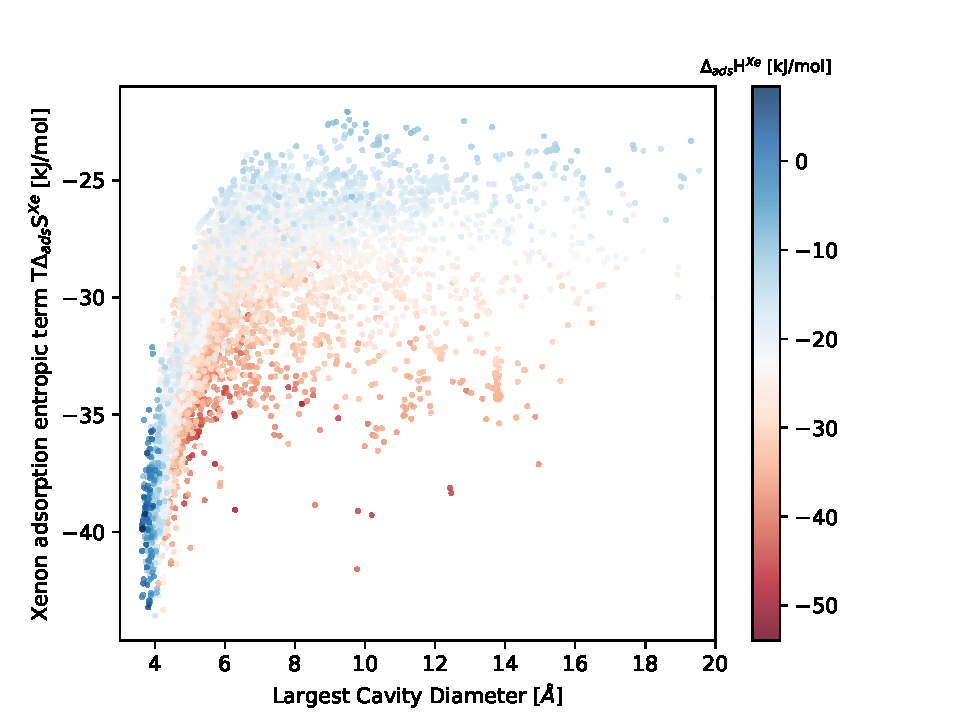
\includegraphics[width=0.48\textwidth]{figures/2-thermo/Scatterplot_entropy_lcd.pdf}
  \hfill
  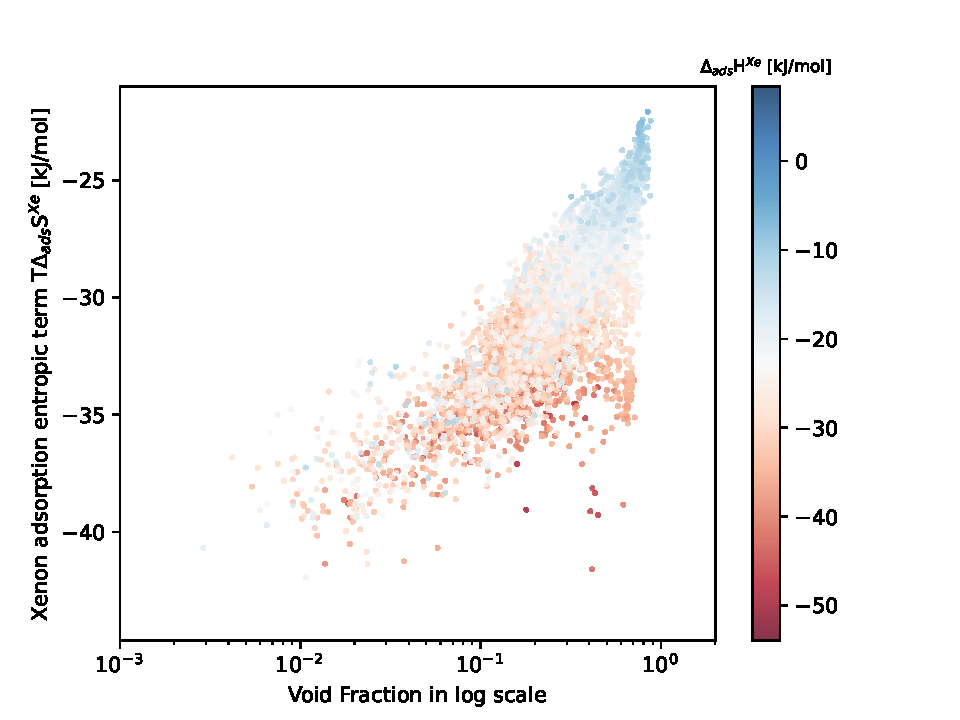
\includegraphics[width=0.48\textwidth]{figures/2-thermo/Scatterplot_entropy_vf.pdf}
  \caption{Comparison plots of the entropic term $T\Delta\e{ads}S\ex{Xe}\e{0}$ at infinite dilution and two geometric descriptors: the LCD\e{UFF} (left) and the void fraction (right).}\label{fgr:entropy_geometry}
\end{figure}

Cross-referencing these findings with the previous results obtained on the influence of geometric descriptors in the section~\ref{sct:geometry}, it becomes evident that the entropic effect aligns with the  enthalpic term in explaining selectivity when the pore size approaches that of xenon. The confinement of xenon within the pores leads to lower entropy in the adsorbed phase compared to the gas phase, especially for pores tailored to xenon's size. Furthermore, the optimal interaction between xenon and the surrounding framework atoms reduces the enthalpic term. Both factors work in concert, elucidating the optimal selectivity observed for this particular pore size value (around \SI{5}{\angstrom}). 

The key takeaways from this section revolve around two relationships. Firstly, there is a correlation between the Henry constant of xenon and selectivity, allowing for rough estimation of Xe/Kr selectivity --- the most selective materials exhibit a strong affinity for xenon. Secondly, the selectivity process is primarily driven by enthalpy --- the separation process has an enthalpic nature as a first-order approximation, which is particularly true for the most selective materials. Analyzing the energy interactions within the material provides crucial insights into its performance. While the focus here has been on thermodynamic properties at infinite dilution, the subsequent section will delve into the impact of pressure on selectivity, specifically examining a 20:80 Xe/Kr mixture at \SI{1}{\atm} and \SI{298}{\kelvin}. 

%%%%
\section{Selectivity drop between two pressure regimes}

As the previous section has established the relationship between selectivity and some geometrical and thermodynamic descriptors, this section focuses on examining the relationship between selectivity values at infinite dilution and selectivity values at ambient pressure using a thermodynamics-based approach. The aim is to gain a better understanding of the underlying mechanisms driving the observed changes in selectivity as previously discussed in Figure~\ref{fgr:SI:overview_2080_9010}. It is worth noting that the findings presented in this section have already been published in Ref.~\cite{Ren_2021}

\subsection{Thermodynamic origins}\label{section:pressure}

After delving into the thermodynamics of the infinite dilution case, the focus now shifts to examining the impact of changes in working pressure on adsorption selectivity and analyzing its underlying thermodynamic mechanisms. Understanding the impact of pressure on selectivity is crucial for accurately assessing adsorption thermodynamics under different working conditions, particularly in specific industrial processes. Insights into the pressure-dependent selectivity may allow for faster screening of materials limited to specific thermodynamic conditions.

\begin{figure}[ht]
  \centering
    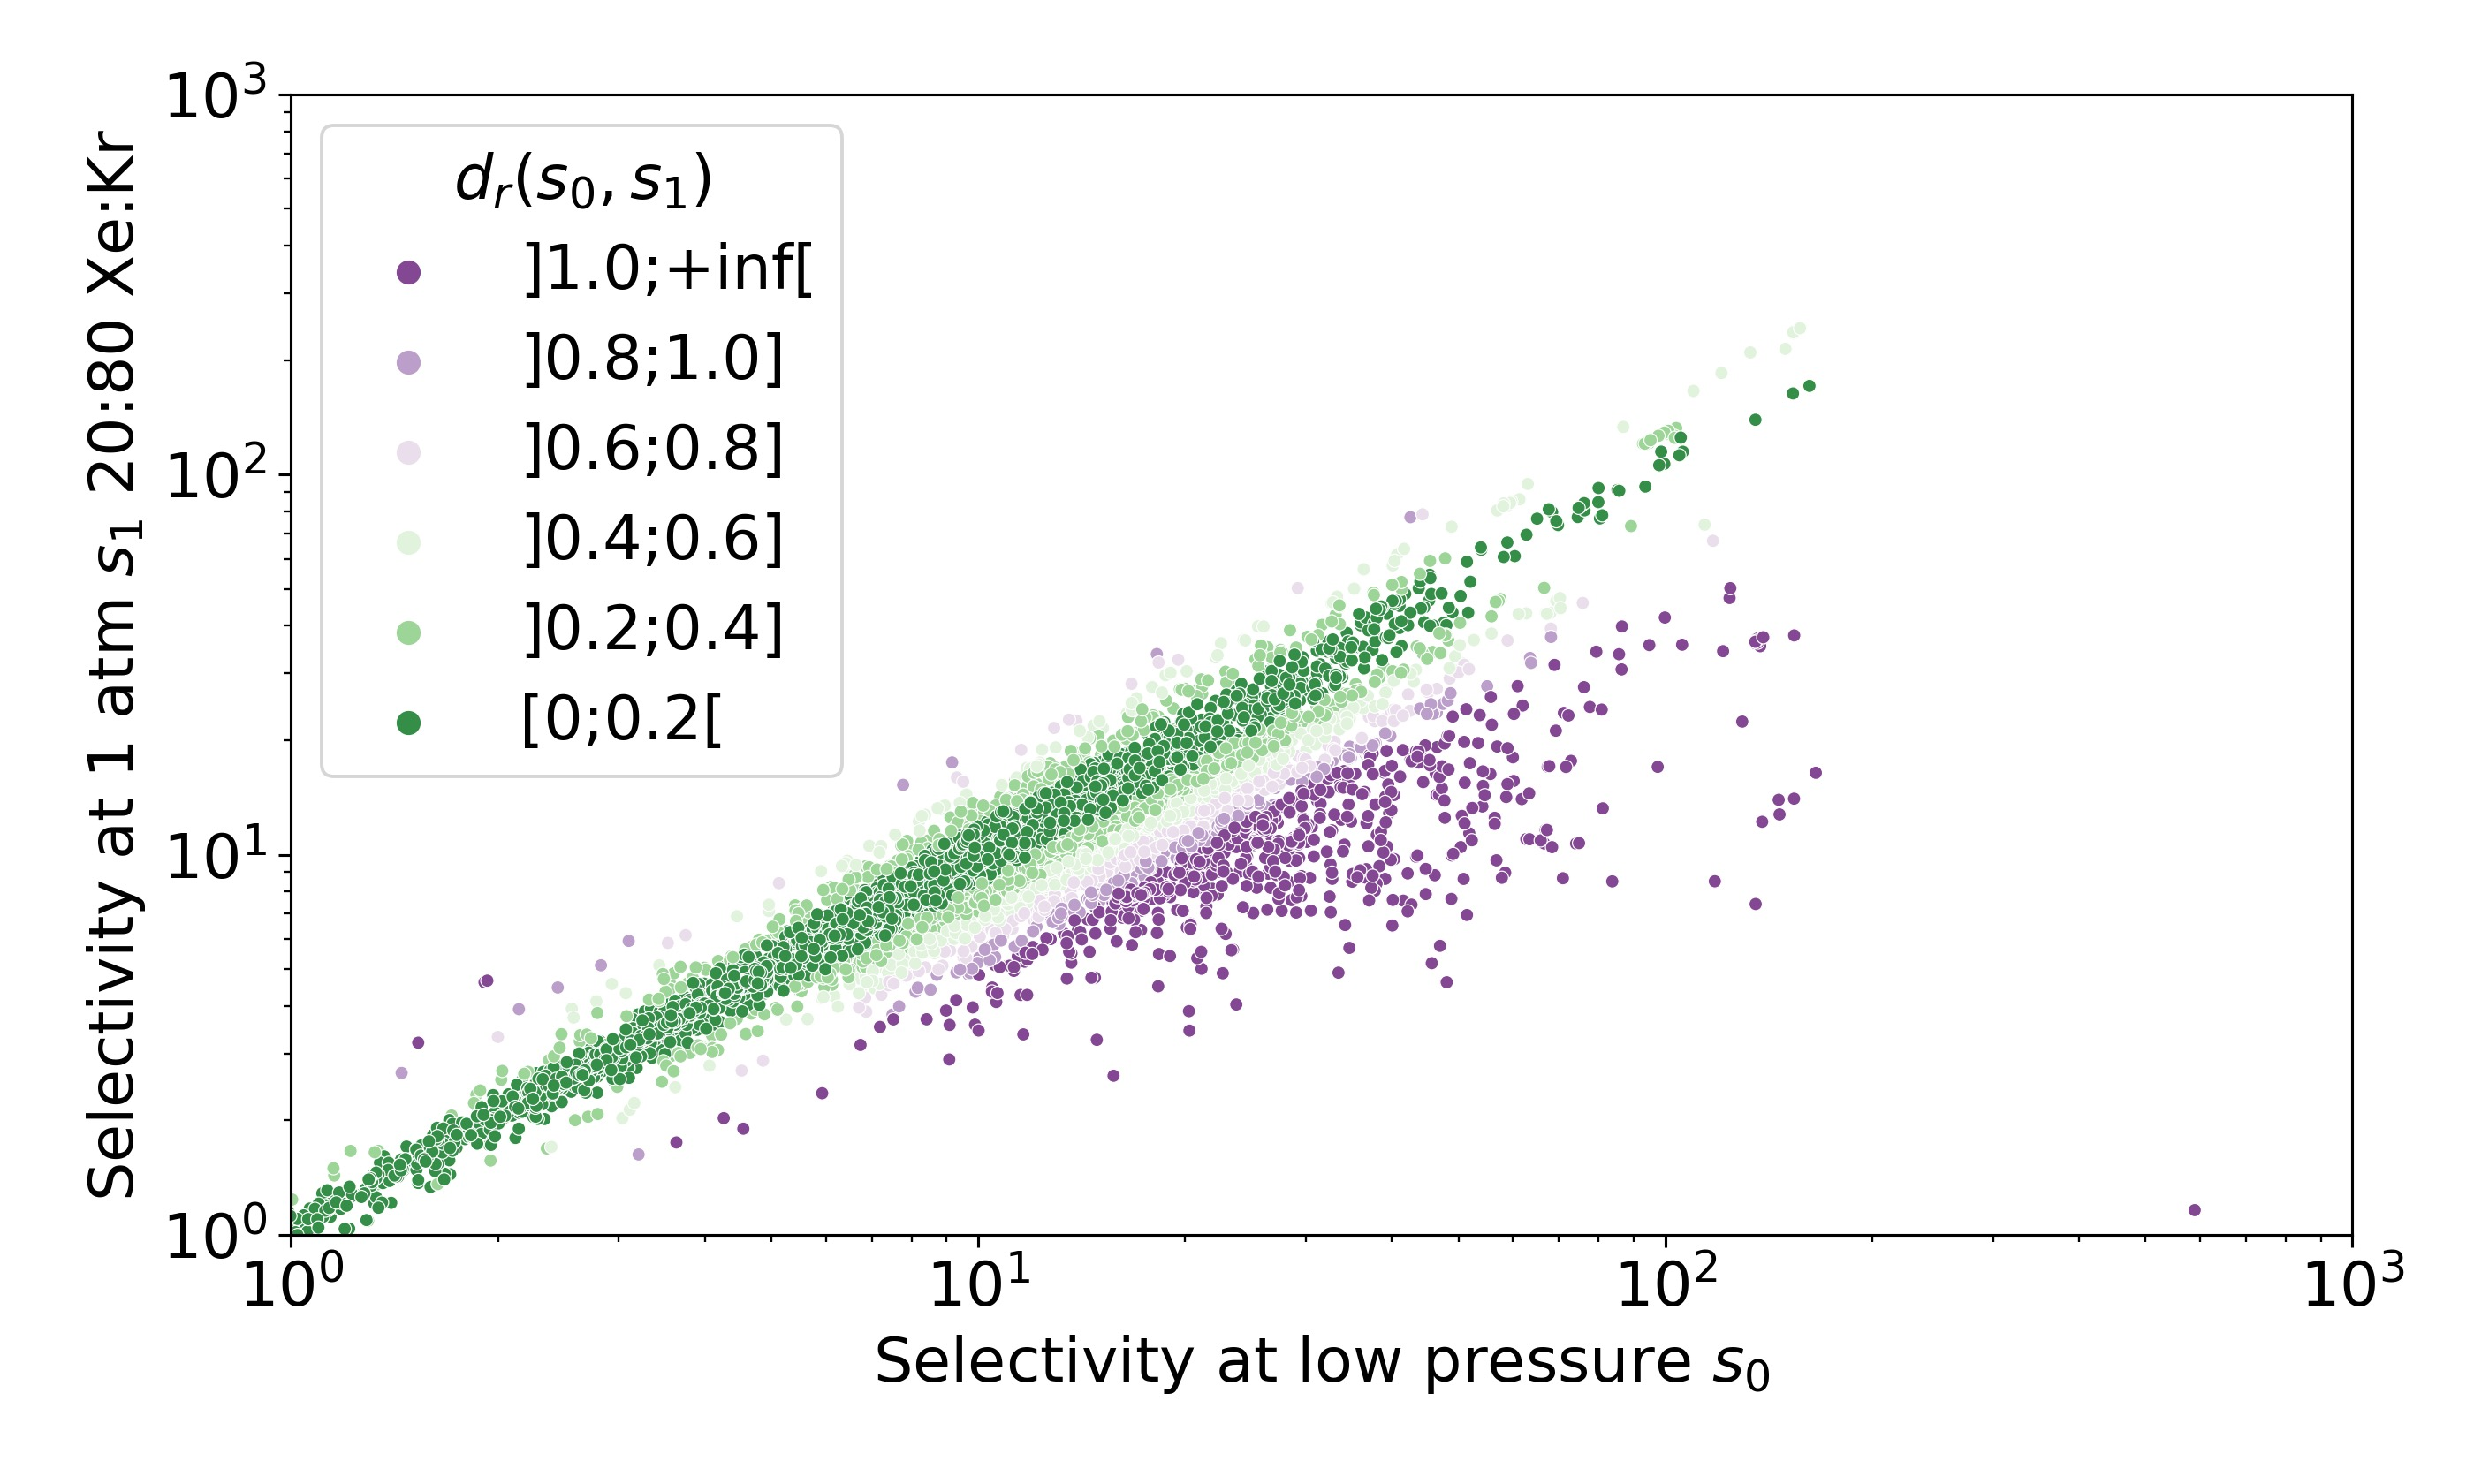
\includegraphics[width=0.6\textwidth]{figures/2-thermo/s_0_vs_s_2080_overview_log.jpg}
    \caption{Difference of selectivity between low pressure and at a \SI{1013}{\hecto\pascal} pressure for a 20:80 xenon/krypton composition. The relative difference between the low-pressure selectivity and the ambient pressure is particularly high for the points labeled in purple.}\label{fgr:overview}
\end{figure}

The selectivity $s\e{1}$ was calculated at a pressure of $1$~atm and ambient temperature using GCMC calculations on the entire dataset, with Xe/Kr mixture composition of 20:80 (found in a byproduct stream from air separation\autocite{kerry2007industrial}), and 90:10 (found in the off-gas streams from nuclear waste\autocite{auerbach2003handbook}). It was observed that for high-selectivity materials, the composition had a minimal impact, as shown in (\emph{cf.} Figure~\ref{fgr:SI:overview_2080_9010}). In the following analysis, the focus is primarily on the selectivity for the 20:80 mixture, which is the most commonly studied composition in the literature. To quantify the difference in selectivity between low and ambient pressures, a relative difference $d_r(s\e{0},s\e{1})$ is considered, as defined in equation~\ref{eq:reldiff}.

\begin{equation}\label{eq:reldiff}
    d_r(s\e{0},s\e{1}) = \dfrac{\lvert s\e{0} - s\e{1} \rvert}{\min(s\e{0},s\e{1})}
\end{equation}

Figure~\ref{fgr:overview} presents the selectivity at ambient pressure $s\e{1}$, plotted against its low-pressure counterpart $s\e{0}$ (for materials where $s\e{0} > 1$, as before). The points on the plot are color-coded according to the values of $d_r(s\e{0},s\e{1})$, which are divided into 6 discrete categories for clarity. A broad correlation is observed, particularly near the diagonal line where approximately {61.5\%} of the materials exhibit a difference below {20\%} (close to the $s_0 = s_1$ line). 
However, it is notable that there are considerably more points, approximately ({74.3\%} of the materials with $d_r(s\e{0},s\e{1})\ge 0.2$) below the first bisector ($s_1 < s_0$), indicating that for these materials, the selectivity $s\e{1}$ at 1~atm is significantly lower than the selectivity $s\e{0}$ at low pressure.

This drop in selectivity primarily affects materials with a relatively high selectivity $s\e{0} > 10$ (Figure~\ref{fgr:overview}). It highlights the potential pitfalls of relying solely on pure-component Henry's constant (i.e., zero-pressure selectivity) for materials screening. While calculating low-pressure selectivity is simpler and faster, it can lead to overestimated selectivity by more than {100\%} in a significant number of materials (646 out of 9,668 in our dataset). To understand the underlying reasons for these shifts in selectivity, a thermodynamic approach will be employed.

Before delving deeper in the analyses of the thermodynamic origins of this pressure-induced selectivity drop, this paragraph will open a small aside on the 90:10 mixture composition.
When examining the 90:10 composition, it becomes apparent that the drop in selectivity is even more pronounced. The selectivity for the higher xenon proportion was already found to be higher than that for the 20:80 composition (Figure~\ref{fgr:compo}). This drop can be attributed to the presence of more or less favorable adsorption sites. In some materials (labeled in purple), at low xenon content composition, xenon and krypton primarily compete for the most favorable sites until these sites become saturated, leaving no xenon to compete in the less selective sites. As the Xe/Kr ratio increases, these less selective nanopores contribute to an overall decrease in selectivity. When combined with the effect of increased pressure, certain materials undergo both phenomena, resulting in a more pronounced drop in selectivity compared to the selectivity at low pressure. These explanations are backed up by the following analyses on the pressure effect, which highlights similar effects of the total pressure (instead of partial pressure) on selectivity --- a higher xenon content is actually equivalent to increasing the partial pressure of xenon. Now that the effect of higher xenon content has been characterized, the following analyses will be based on the 20:80 Xe/Kr composition.

\begin{figure}[t]
  \centering
    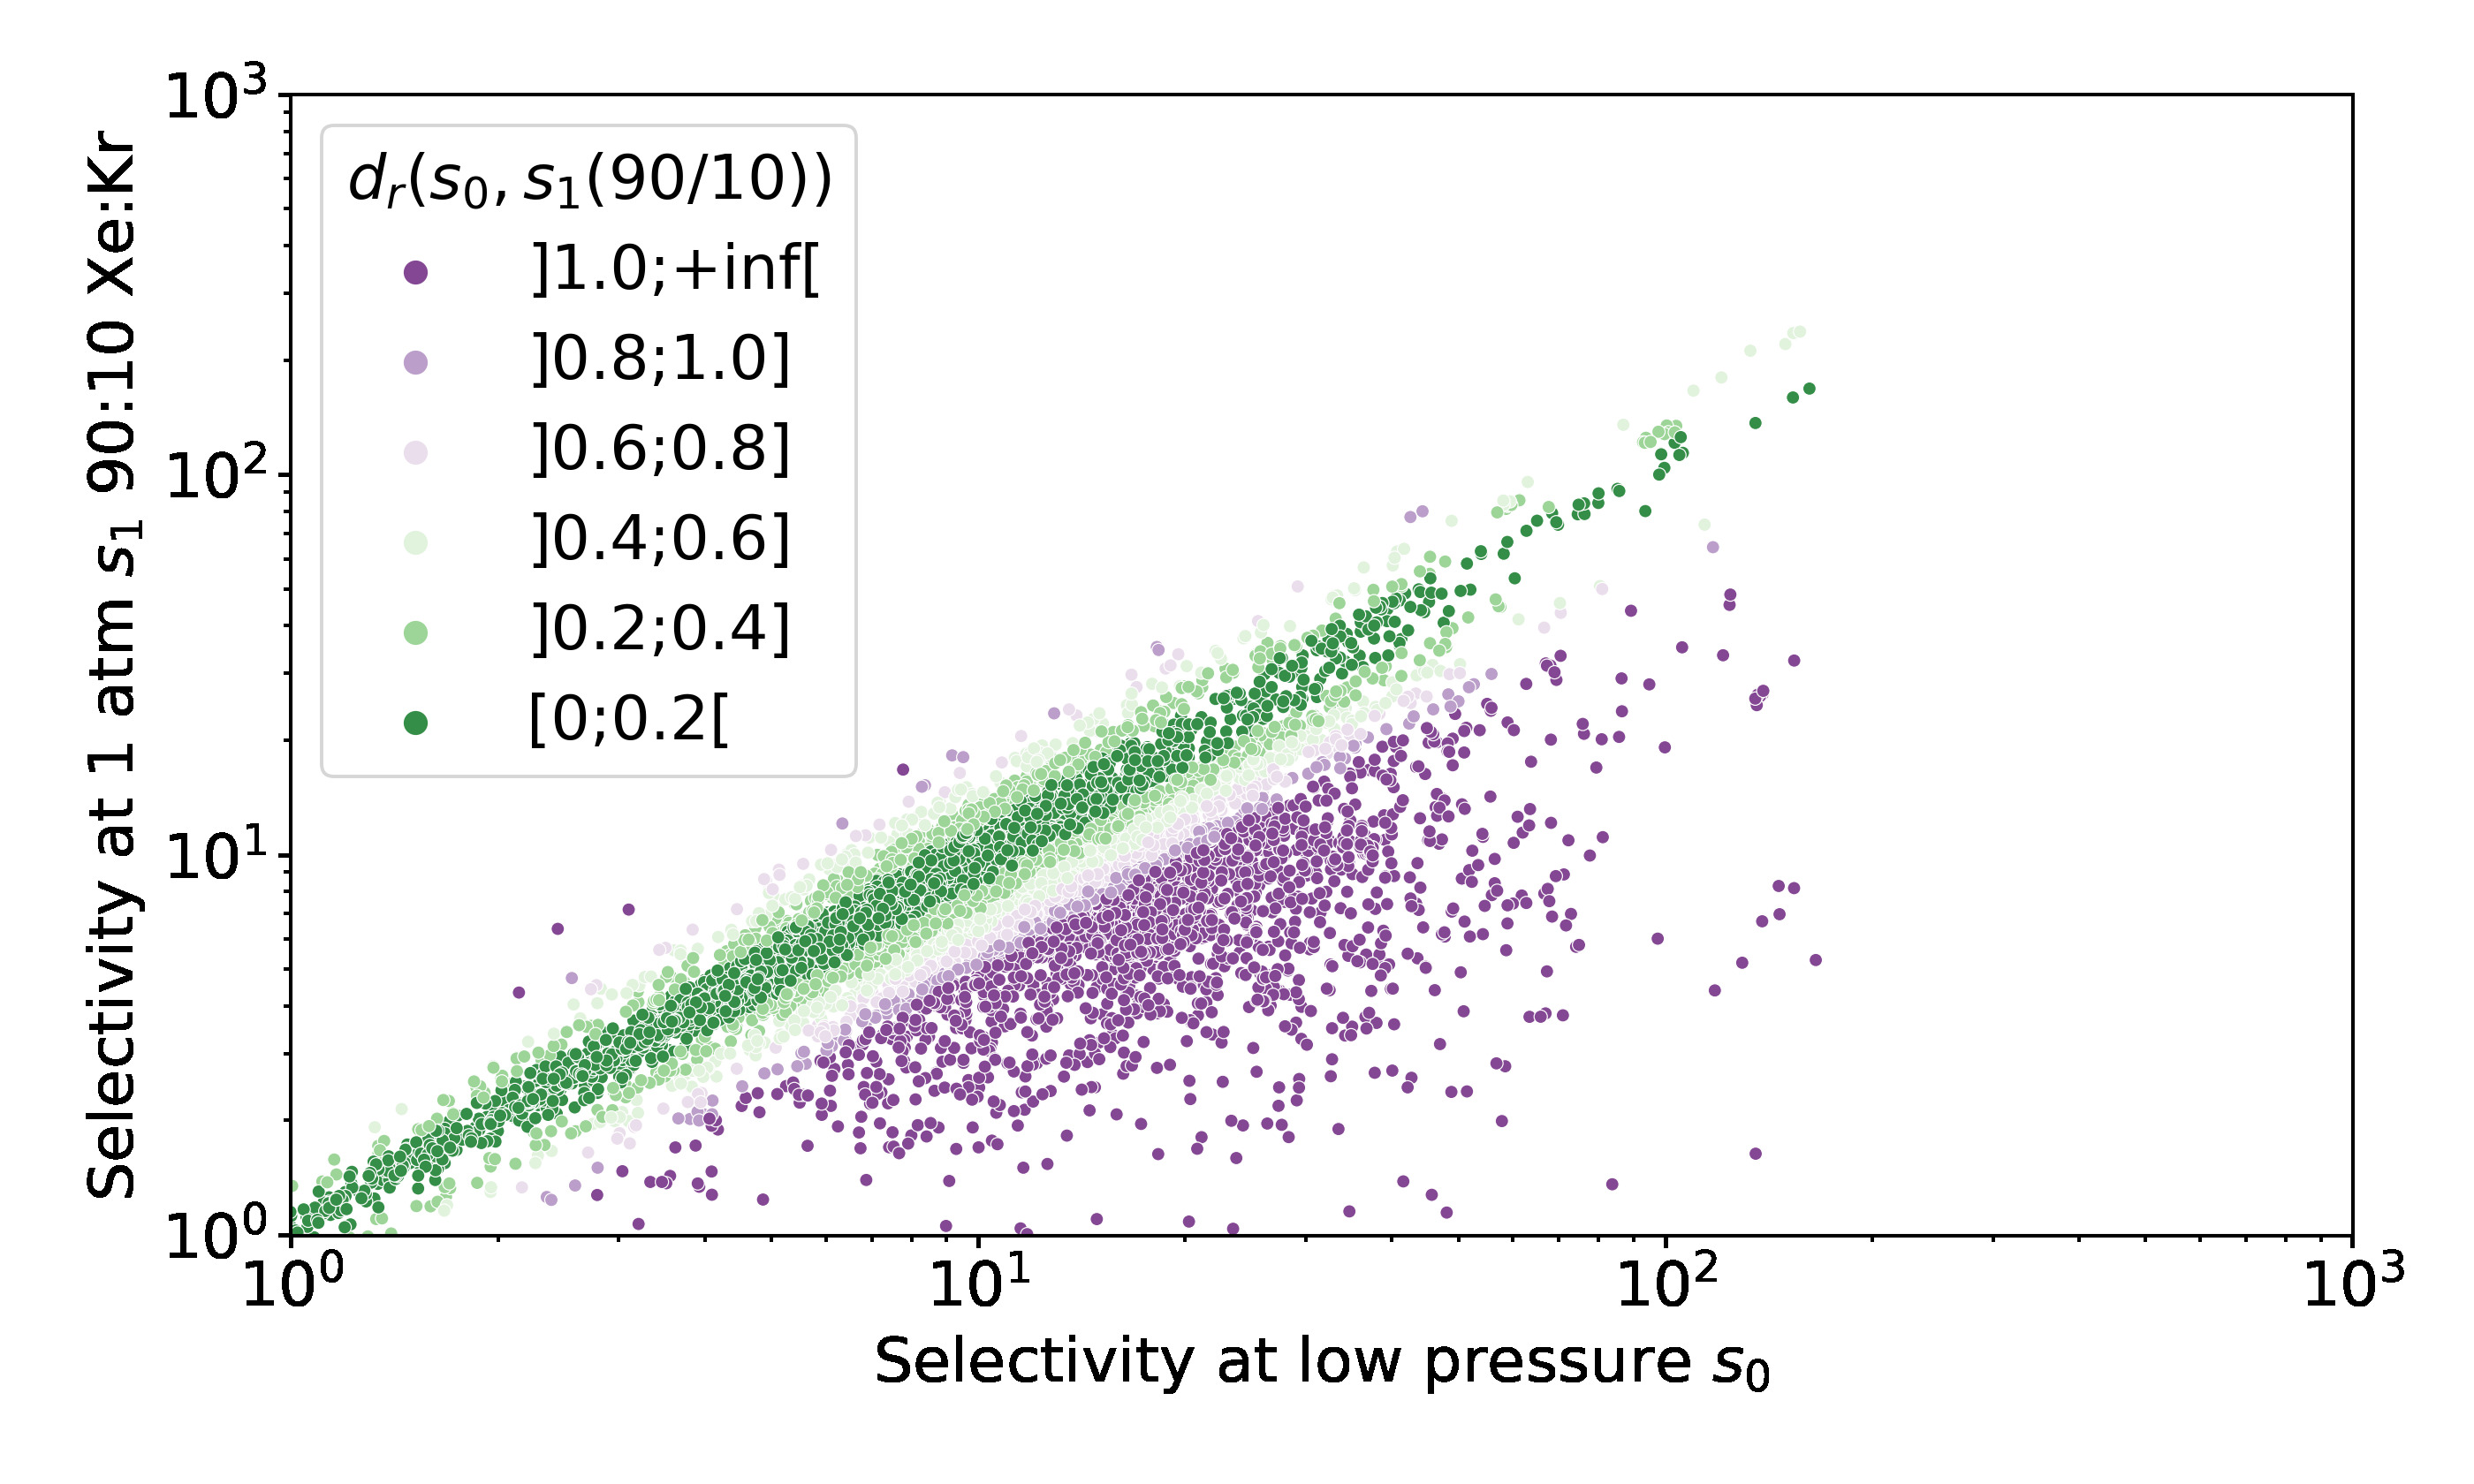
\includegraphics[width=0.6\textwidth]{figures/2-thermo/s_0_vs_s_9010_overview_log.jpg}
    \caption{Difference of selectivity between low pressure and at a \SI{1013}{\hecto\pascal} pressure for a 90:10 xenon/krypton composition. The relative difference between the low-pressure selectivity and the ambient pressure is particularly high for the points labeled in purple.}\label{fgr:overview_9010}
\end{figure}

To quantitatively assess the thermodynamic effects involved in the competitive adsorption under different regimes (for the 20:80 composition), thermodynamic properties of the ``exchange equilibrium'' predefined in equation~\ref{eq:exchange} are considered. Figure~\ref{fgr:HSplot_0} displays a scatterplot of the exchange entropy at low pressure, represented as $T\Delta\e{exc}S\e{0}$, plotted against the exchange enthalpy $\Delta\e{exc}H\e{0}$. The points on the plot are color-coded according to the selectivity $s\e{0}$ (with discrete categories for clarity), which is related to the enthalpy and entropy through Equation~\ref{eq:exc_entropy} --- indicating iso-selectivity lines correspond to parallel straight lines in this scatterplot.
  
\begin{figure}[t]
\centering
  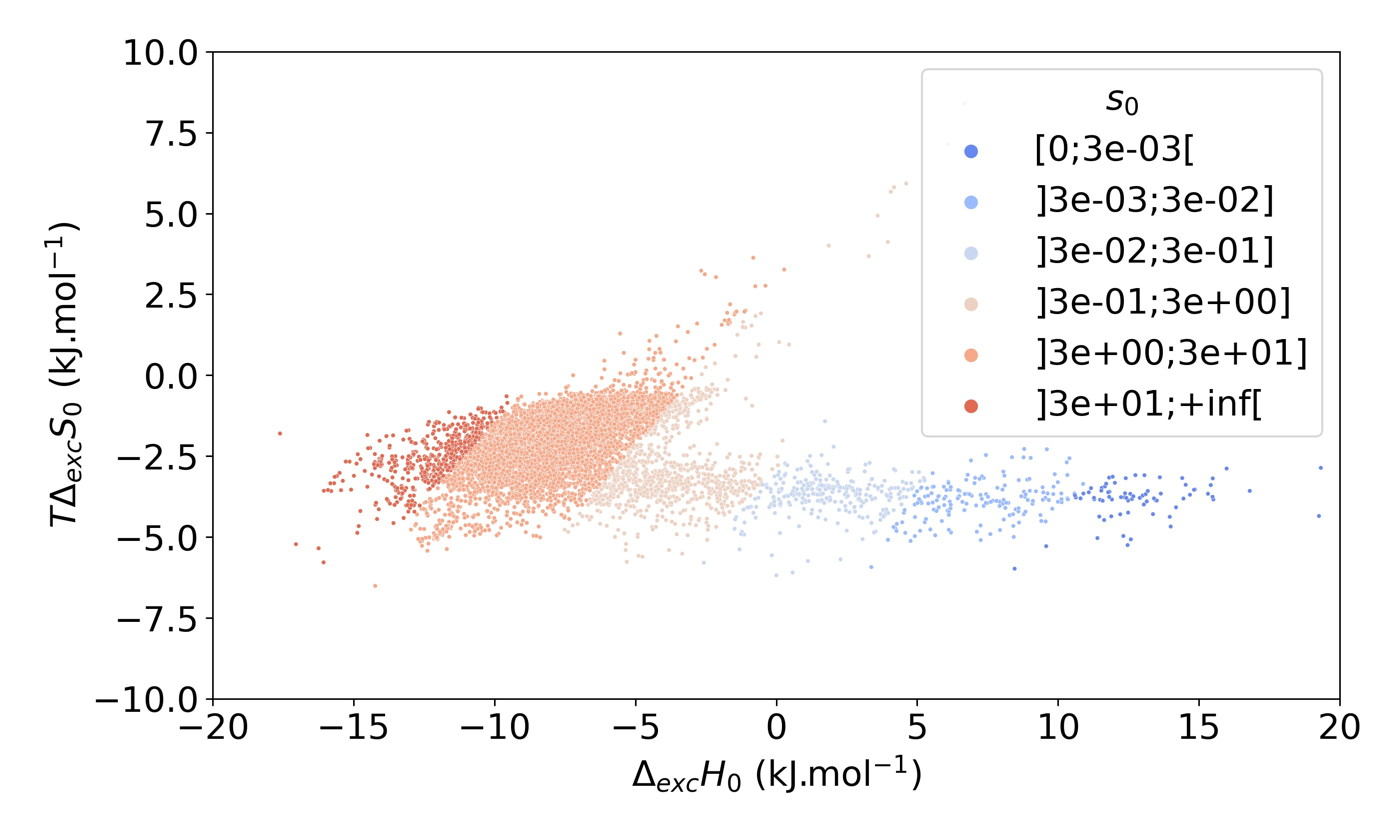
\includegraphics[width=0.6\textwidth]{figures/2-thermo/enthalpy_entropy_0_s_0.jpg}
  \caption{The energetic equivalent of exchange entropy $T\Delta\e{exc}S\e{0}$ and enthalpy $\Delta\e{exc}H\e{0}$ at low pressure labeled using the selectivity $s\e{0}$ at low pressure (for any xenon/krypton composition). The limit between labels follows an affine function of slope $1/T$ and of intercept $-R\ln(s\e{0}\ex{lim})$ where $s\e{0}\ex{lim}$ is the limit selectivity value (\emph{cf.} equation~(\ref{eq:exc_entropy})). In other words, the iso-selectivity lines are all parallel lines of equation $y=f(x)$ where $f$ is the affine function described previously.}\label{fgr:HSplot_0}
\end{figure}


Figure~\ref{fgr:SI:dist0} presents the distributions of the exchange enthalpy and entropy at low pressure. Among the 630 most selective materials ($s\e{0} > 30$), the distribution of the exchange enthalpy $\Delta\e{exc}H\e{0}$ is centered around $-12.0$\,\si{\kilo\joule\per\mol} with a standard deviation of $1.3$\,\si{\kilo\joule\per\mol}. On the other hand, the distribution of the exchange entropy (represented as $T\Delta\e{exc}S\e{0}$) is centered around $-2.5$\,\si{\kilo\joule\per\mol}, with a standard deviation of $0.7$\,\si{\kilo\joule\per\mol}. These figures, along with the overall distribution plotted in Figure~\ref{fgr:HSplot_0}, provides further evidence of the relatively modest role of entropy in determining the selectivity at low pressure, which corresponds, on average, to approximately {$20$\%} of the exchange enthalpy.

Examining Figure~\ref{fgr:SI:dist1} for the selectivity at ambient pressure, similar conclusions can be drawn regarding the limited influence of entropy on selectivity values. The distribution of the entropic term $T\Delta\e{exc}S\e{1}$ is centered around $-3$~\si{\kilo\joule\per\mole}, which remains relatively small compared to the values of $\Delta\e{exc}H\e{1}$. For the most selective materials, the entropic term represents approximately {$19$\%} of the exchange enthalpy $\Delta\e{exc}H\e{1}$ at ambient pressure.

\begin{figure*}[ht]
  \centering
    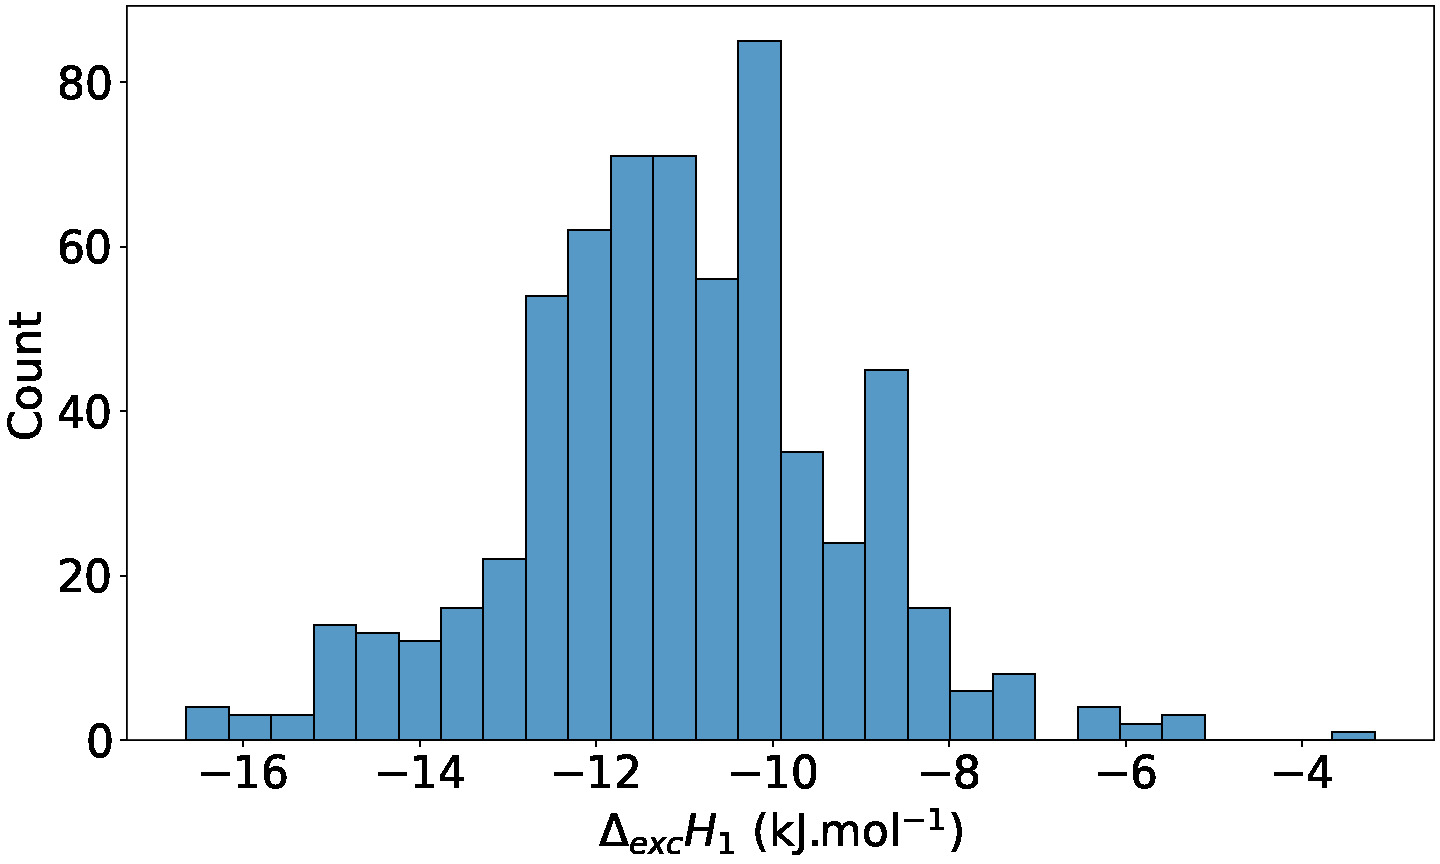
\includegraphics[width=0.45\textwidth]{figures/2-thermo/Delta_H_2080.jpg}
    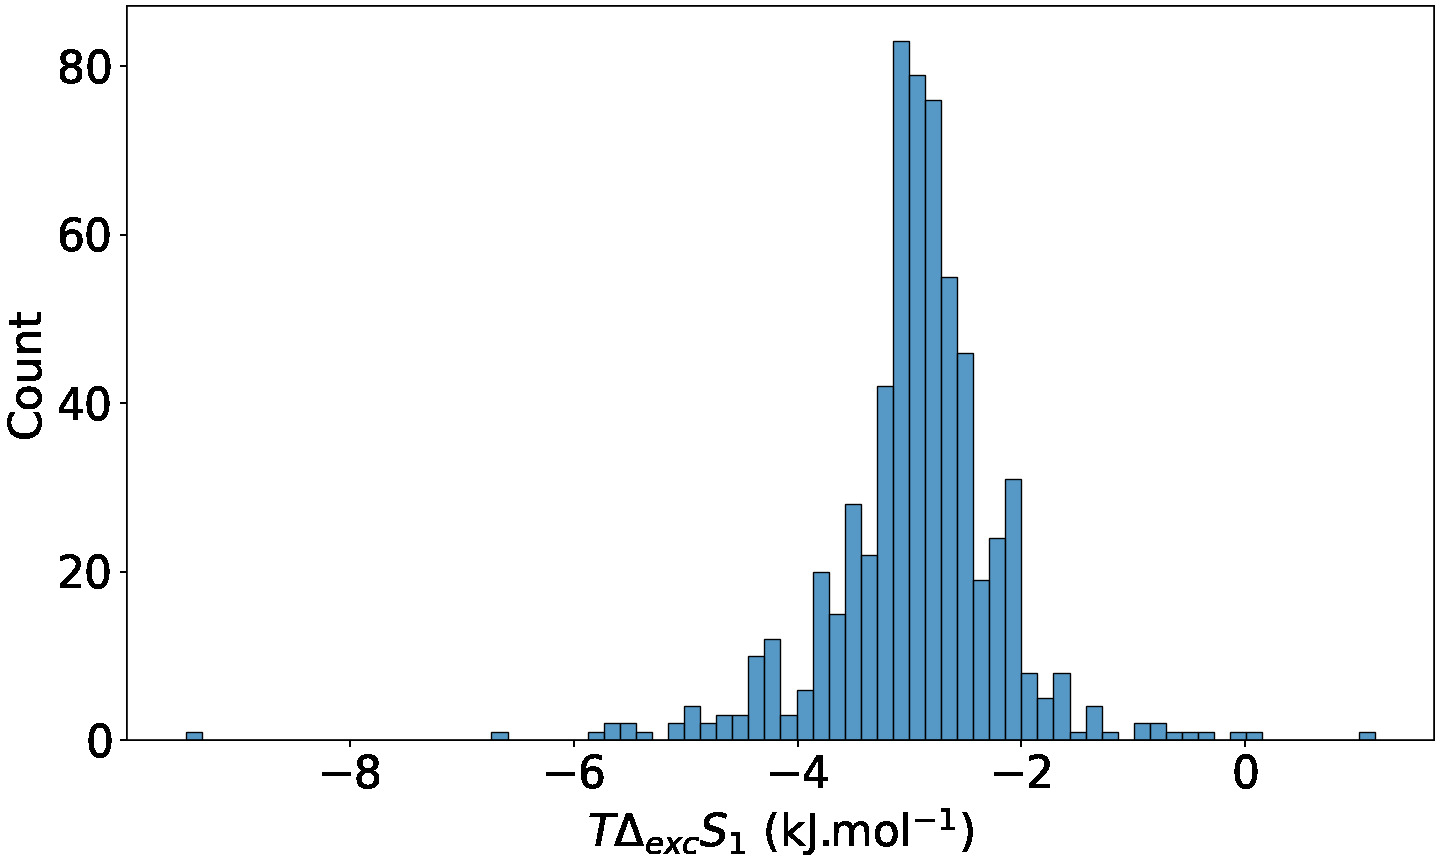
\includegraphics[width=0.45\textwidth]{figures/2-thermo/T_Delta_S_2080.jpg}
    \caption{Distribution of the enthalpy $\Delta\e{exc}H\e{1}$ and entropic term $T\Delta\e{exc}S\e{1}$ of exchange at ambient pressure on the 630 most selective structures.}\label{fgr:SI:dist1}
\end{figure*}

Figure~\ref{fgr:HSplot_1} represents a scatterplot of the exchange entropy at $P = 1$\,atm $\Delta\e{exc}S\e{1}$ against the exchange enthalpy at ambient pressure $\Delta\e{exc}H\e{1}$. The points are color-coded according to the low-pressure selectivity $s\e{0}$ to compare it with the Fig.~\ref{fgr:HSplot_0}. In comparison to the iso-selectivity $s\e{1}$ straight parallel lines (\emph{cf.}~Figure~\ref{fgr:SI:HS_split}), it can be observed that many materials with high $s\e{0}$ have lower $s\e{1}$, as indicated by a migration of points to the right of the plot. This shift is thus mainly due to a higher (less favorable) exchange enthalpy, implying that enthalpy plays a crucial role in determining selectivity at higher pressures.

\begin{figure}[ht]
  \centering
    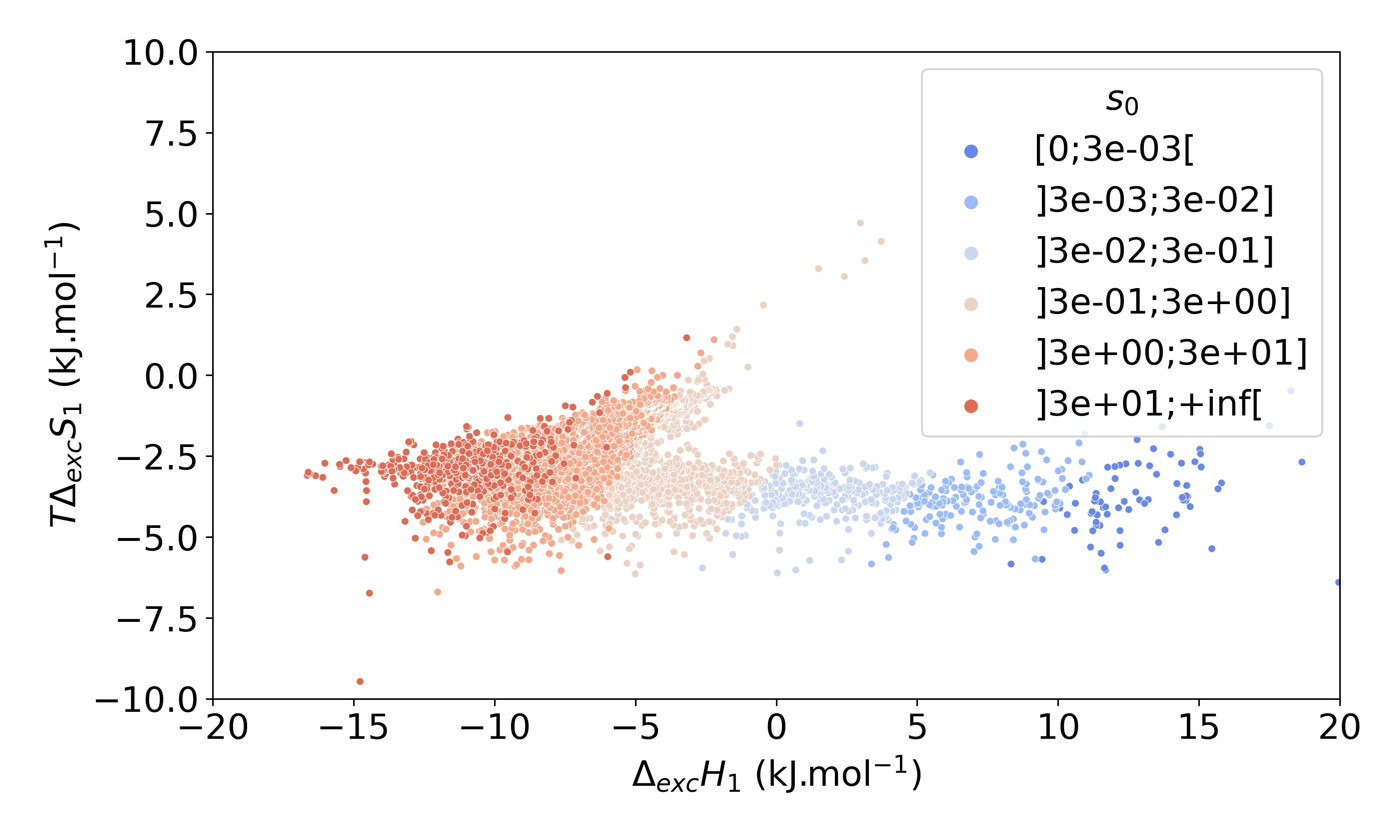
\includegraphics[width=0.6\textwidth]{figures/2-thermo/enthalpy_entropy_2080_s_0.jpg}
    \caption{The energetic equivalent of exchange entropy $T\Delta\e{exc}S\e{1}$ and enthalpy $\Delta\e{exc}H\e{1}$ at ambient pressure (for a 20:80 xenon/krypton composition) labeled using the selectivity $s\e{0}$ at low pressure. The points are layered so that the points with higher $s\e{0}$ are always above. To see a split version of this plot, please refer to Figure~\ref{fgr:SI:HS_split}.}\label{fgr:HSplot_1}
  \end{figure}
 
To quantify this change, the distributions of the exchange enthalpy $\Delta\e{exc}H\e{1}$ and the energetic equivalent of the exchange entropy $T\Delta\e{exc}S\e{1}$ at ambient pressure (Figure~\ref{fgr:SI:dist1}) are considered. The enthalpy distribution $\Delta\e{exc}H\e{1}$ is now centered at $-11.1$\,\si{\kilo\joule\per\mol} with a standard deviation of $1.9$\,\si{\kilo\joule\per\mol}. In comparison to the zero-pressure values, the enthalpy distribution exhibits greater dispersion, suggesting significant changes in individual values and an overall increase in average enthalpy. Most materials display lower selectivity at ambient pressure due to enthalpic effects, which can be attributed to the general increase in adsorption enthalpy with increasing gas phase loading, which is linked to the presence of more adsorbed molecules. The correlations shown in Figure~\ref{fgr:histo_K} suggest that highly selective materials have a high affinity for xenon, resulting in substantial uptake at \SI{1}{\atm}. The large Xe loading means the saturation of the most favorable adsorption sites and the subsequent adsorption of weaker host--guest interactions contribute to an overall increase in average adsorption enthalpy at non-zero loading.

 
\begin{figure*}[ht]
  \centering
    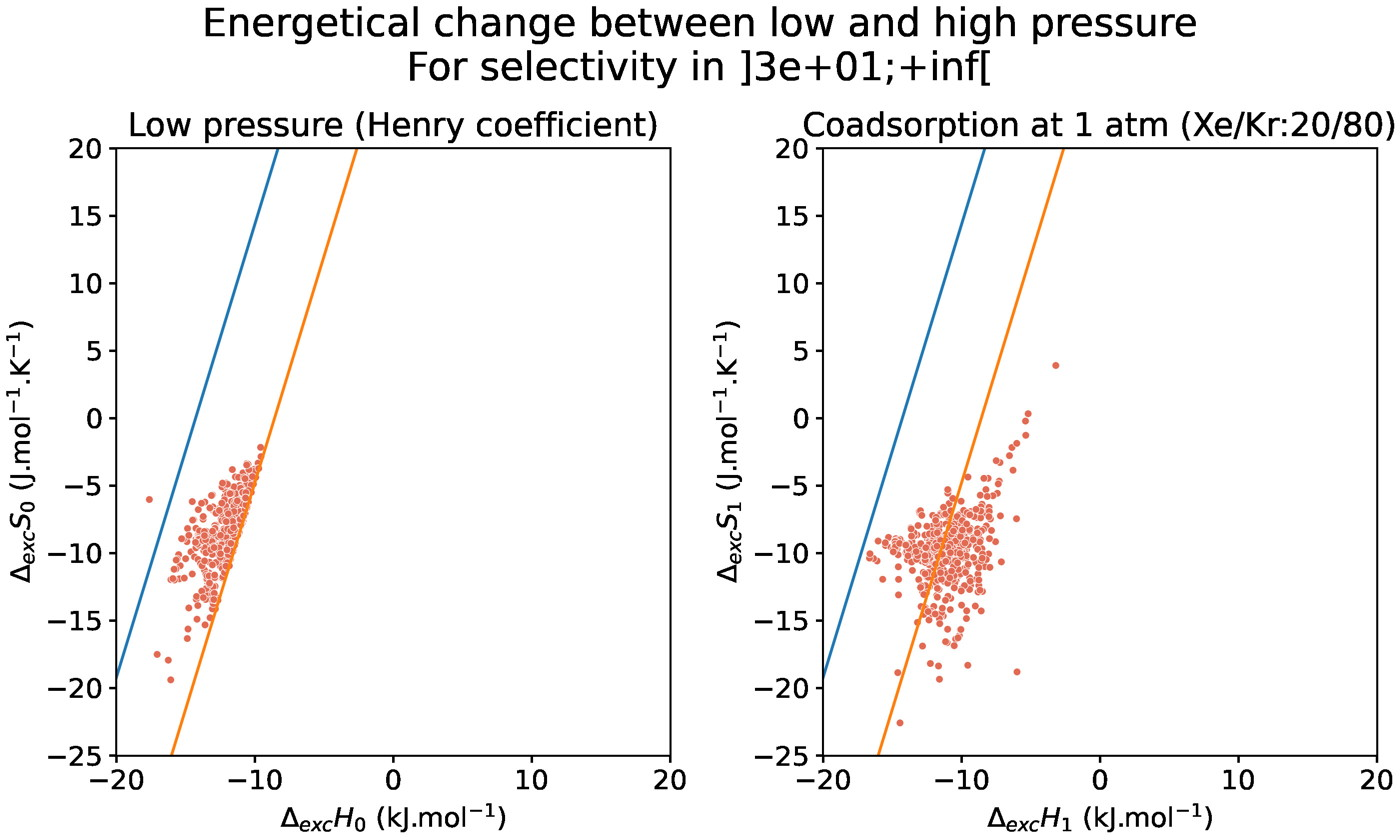
\includegraphics[width=0.45\textwidth]{figures/2-thermo/H_S_0.jpg}
    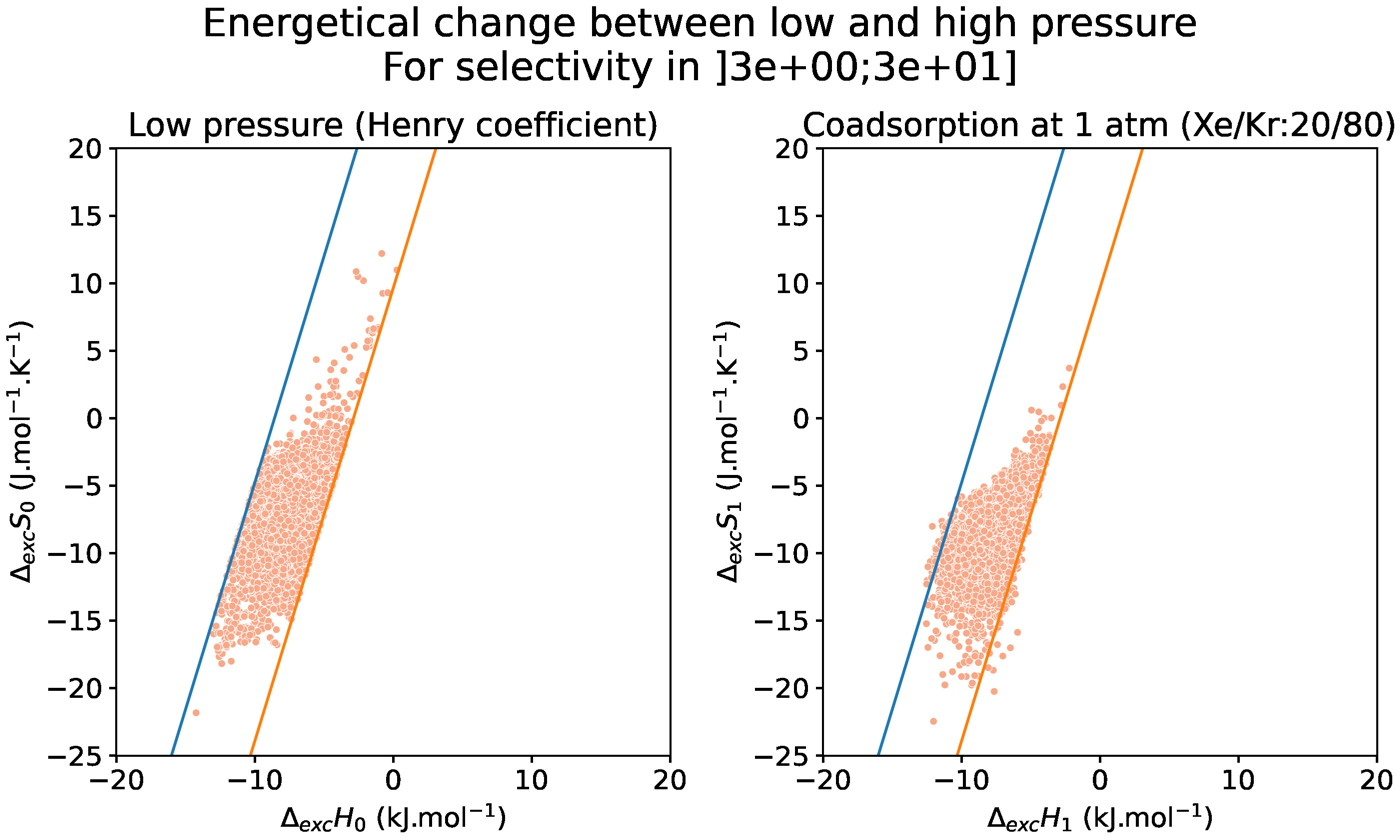
\includegraphics[width=0.45\textwidth]{figures/2-thermo/H_S_1.jpg}
    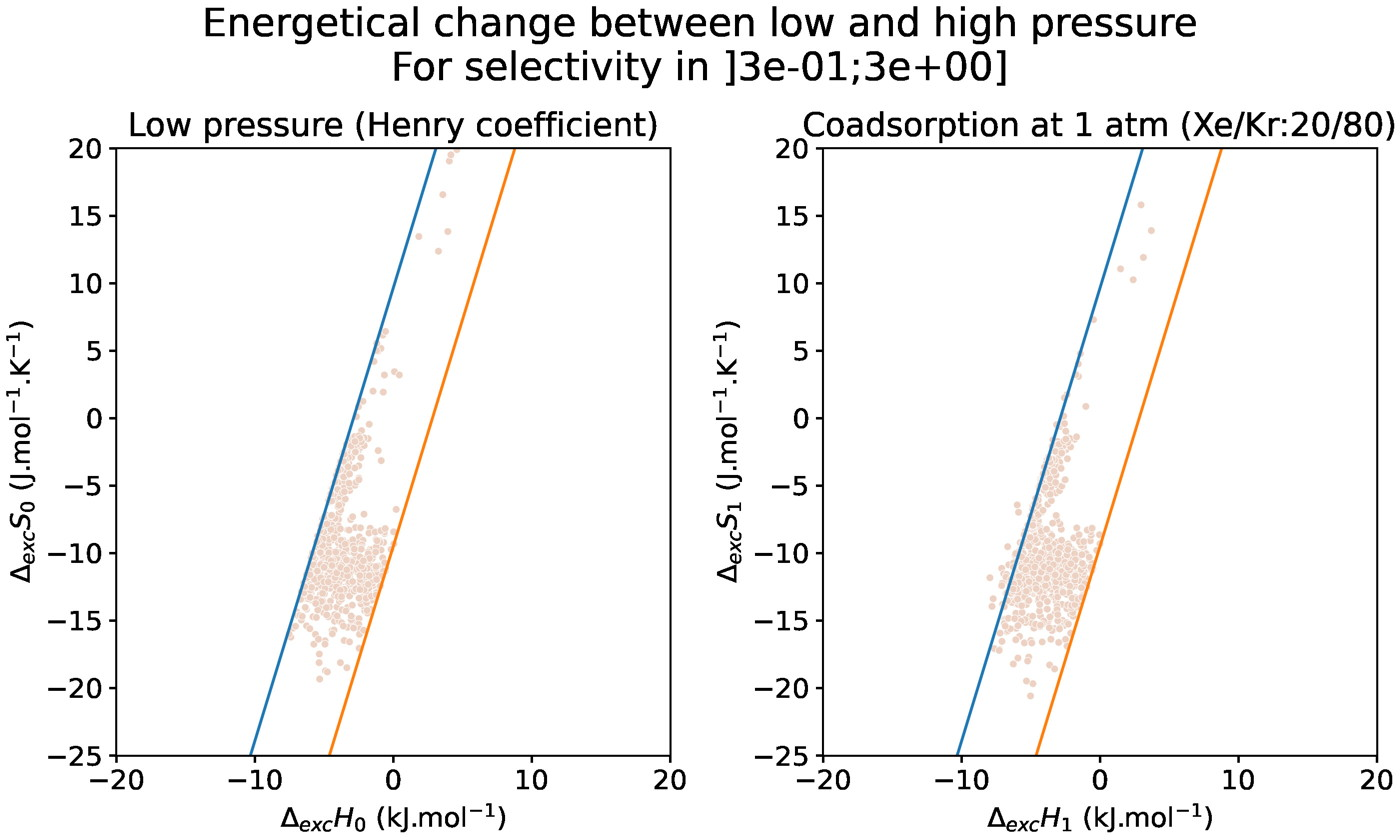
\includegraphics[width=0.45\textwidth]{figures/2-thermo/H_S_2.jpg}
    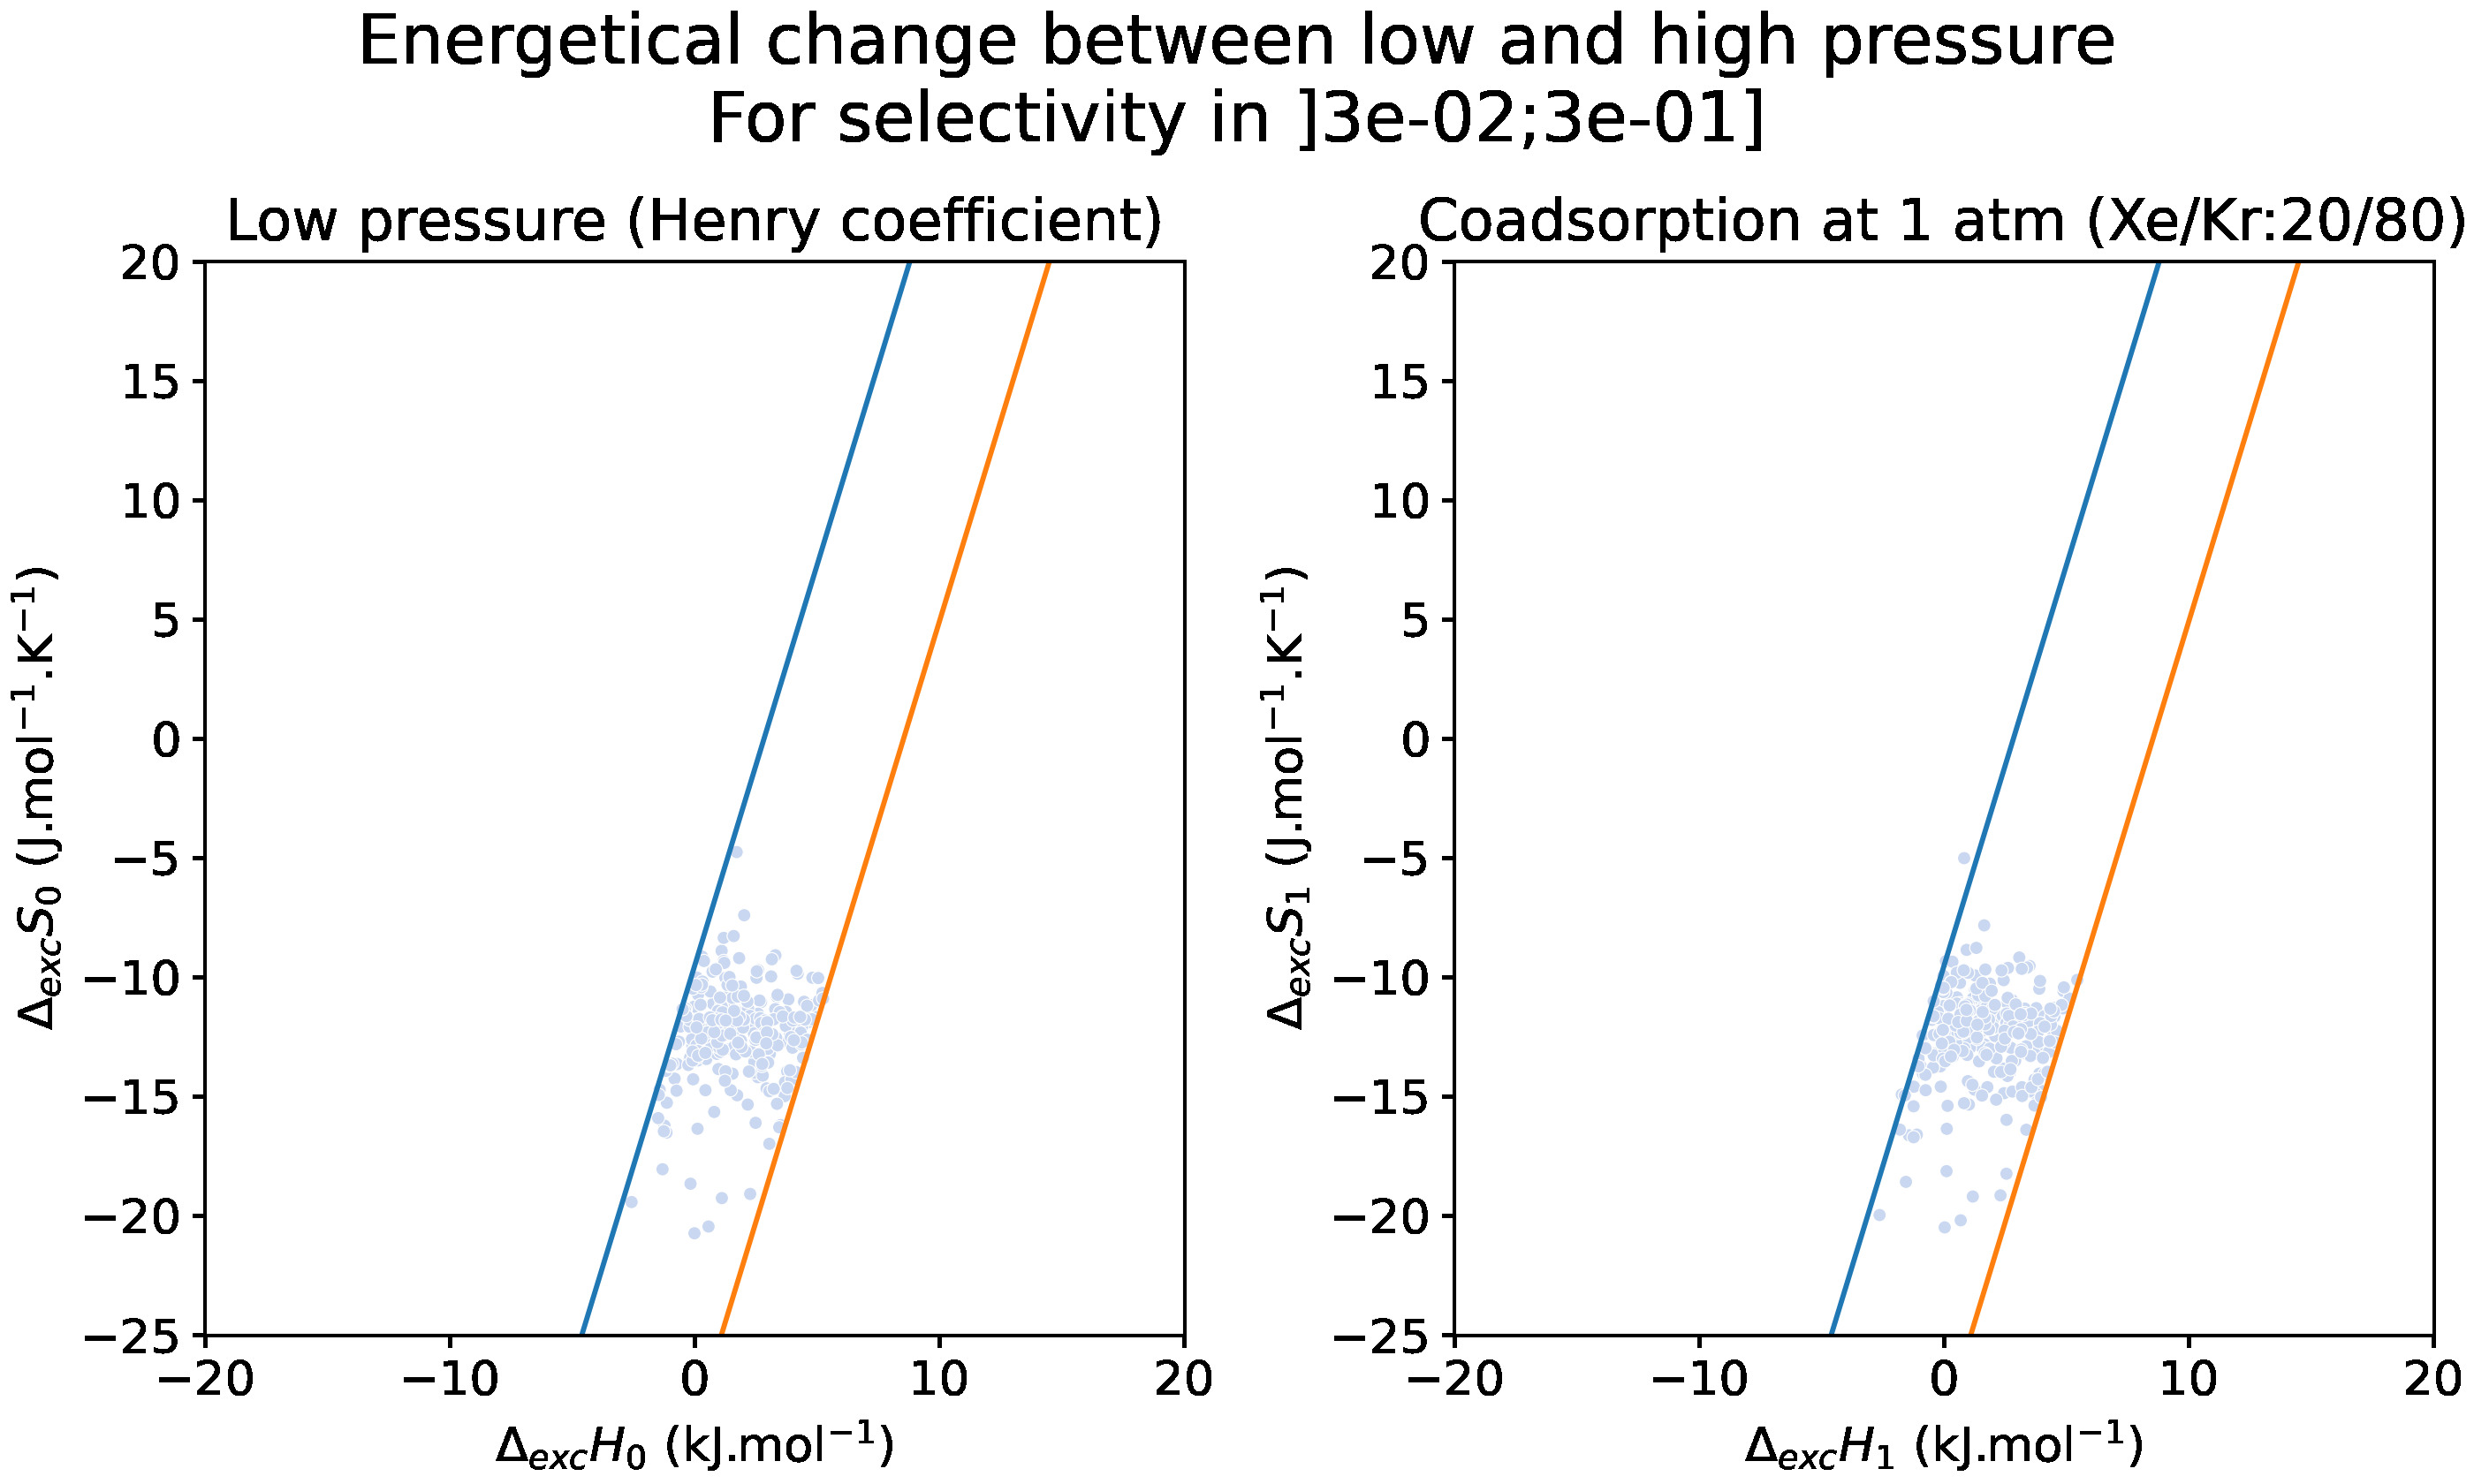
\includegraphics[width=0.45\textwidth]{figures/2-thermo/H_S_3.jpg}
    \caption{Split view of Figure~\ref{fgr:HSplot_0} and~\ref{fgr:HSplot_1}. The iso-selectivity lines for the limit considered are represented with blue and orange lines. It seems that the shift in exchange enthalpy for the structures with a selectivity higher than $30$.}\label{fgr:SI:HS_split}
\end{figure*}

The entropic term $T\Delta\e{exc}S\e{1}$ is now centered at $-2.9$\,\si{\kilo\joule\per\mol}, with a standard deviation of $0.8$\,\si{\kilo\joule\per\mol} (almost unchanged from low-pressure). The average entropy is lower, indicating a less favorable separation overall due to entropic effects. This evolution of the entropic term suggests the possibility of a reorganization of adsorbed molecules within each material. However, the difference in enthalpy distribution has a greater impact on high-pressure selectivity compared to the distribution of entropy. Thus, the overall contribution of enthalpy appears to be more decisive than the role of entropy in determining selectivity changes, even at ambient pressure. This finding is significant for screening studies, as evaluating adsorption enthalpy computationally is generally faster than determining adsorption free energy (or entropy).

\begin{figure*}[t]
  \centering
    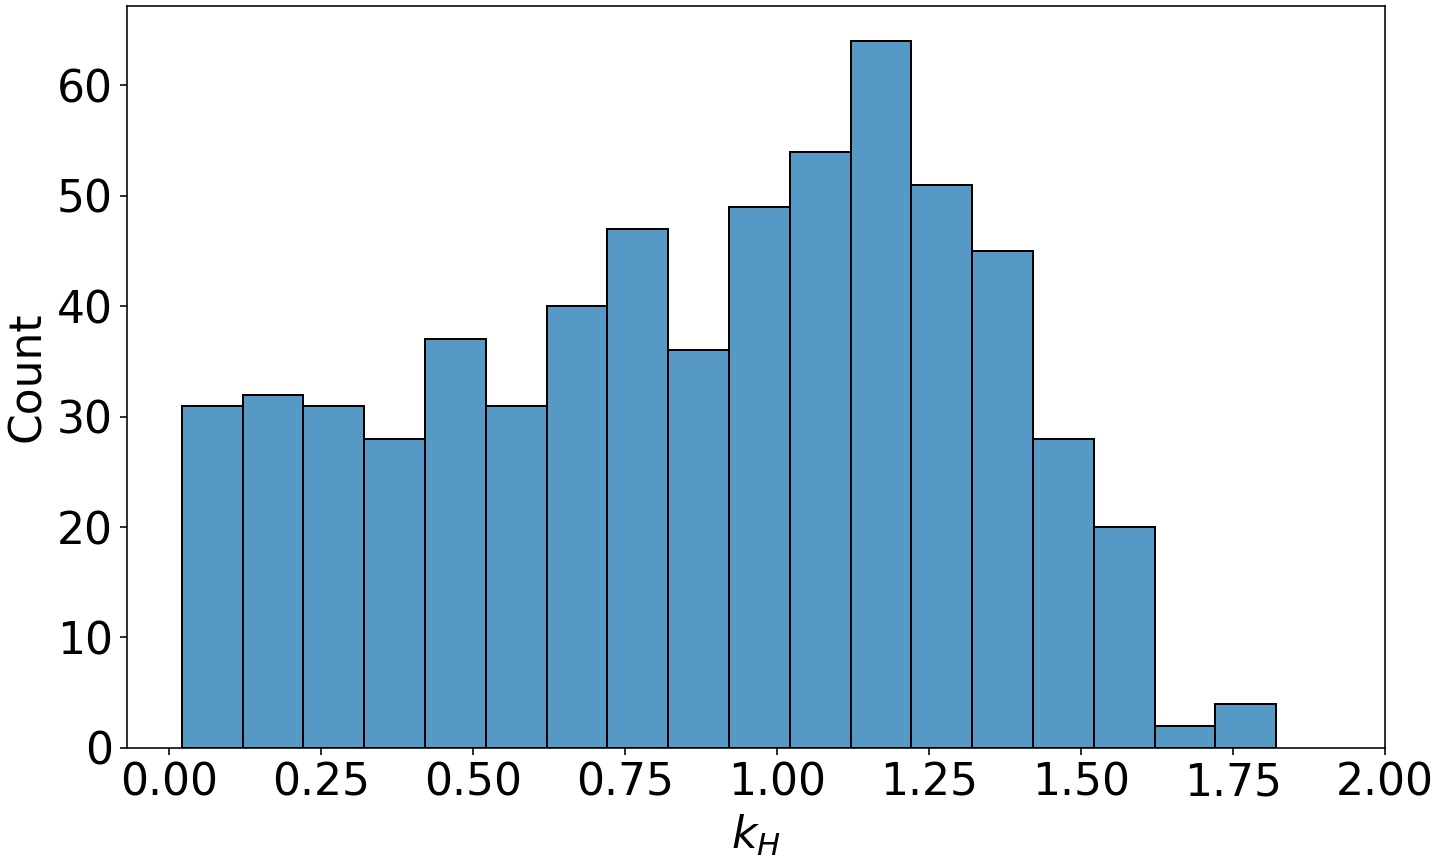
\includegraphics[width=0.37\textwidth]{figures/2-thermo/k_H.jpg}
    \hspace{8mm}
    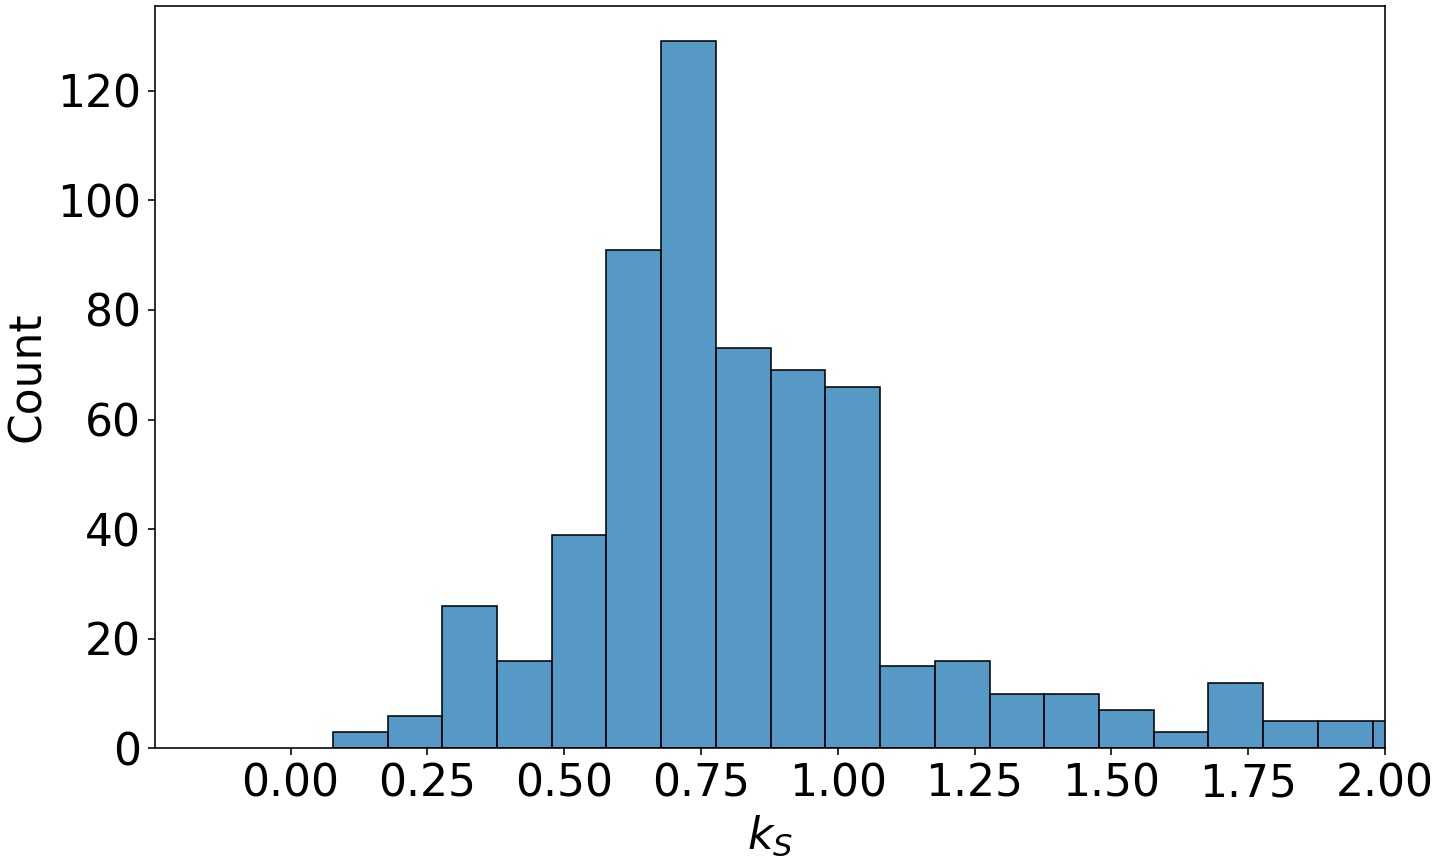
\includegraphics[width=0.37\textwidth]{figures/2-thermo/k_S.jpg}
    \caption{Distribution of the enthalpic $k\e{H}$ and entropic $k\e{S}$ contributions to the change of selectivity from low to ambient pressure for the 630 materials with $s\e{0}>30$. $k\e{H}$ has a rather broad and uniform distribution, whereas $k\e{S}$ has a bell-like distribution. }\label{fgr:distk}
\end{figure*}

\begin{figure}[t]
\centering
  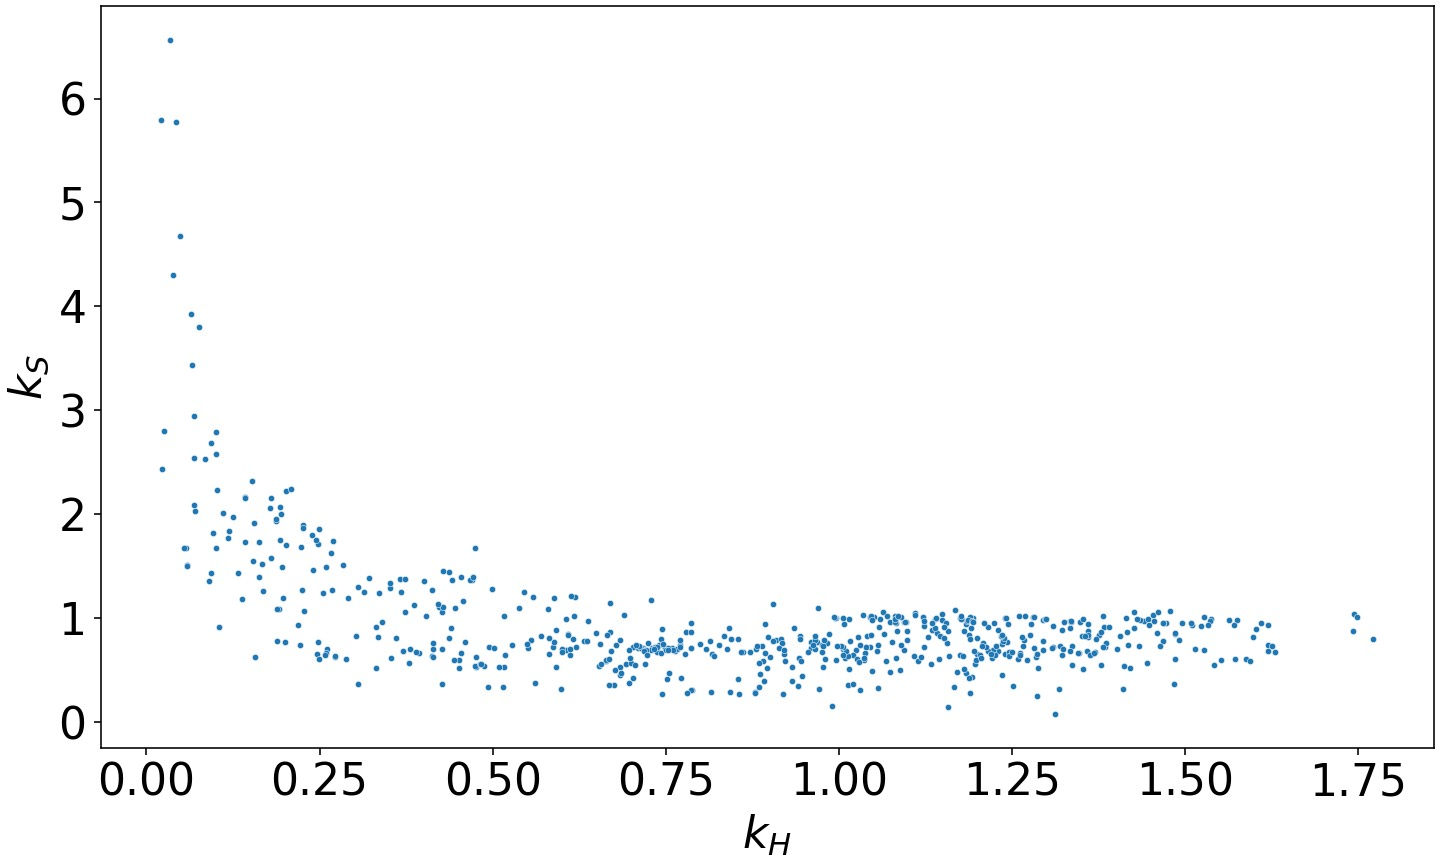
\includegraphics[width=0.45\textwidth]{figures/2-thermo/k_S_vs_k_H.jpg}
  \caption{Scatterplot of the enthalpic contribution $k\e{H}$ and entropic contribution $k\e{S}$ for the 630 materials with $s\e{0}>30$. The entropic compensation occurs when the enthalpic contribution is around $0.1$, else its value is around 1 and has little effect on the selectivity change.}\label{fgr:scatterk}
\end{figure}
  
To further investigate the thermodynamics of the selectivity change, I quantify in this section the contributions of enthalpy and entropy. The ratio ${s\e{1}}/{s\e{0}}$ is equal to the product $k\e{H} \times k\e{S}$ where $k\e{H}$ and $k\e{S}$ are the enthalpic and entropic contributions to the selectivity change defined as:
\begin{equation}
\label{eq:effects}
    \begin{split}
      k\e{H} & = \exp\left(-\dfrac{\Delta\e{exc}H\e{1}-\Delta\e{exc}H\e{0}}{RT}\right) \\ k\e{S} & = \exp\left(\dfrac{\Delta\e{exc}S\e{1}-\Delta\e{exc}S\e{0}}{R}\right)
    \end{split}
\end{equation}
As depicted in Figure~\ref{fgr:distk}, the entropic contribution $k\e{S}$ has a bell-shaped distribution, with a mean of $0.9$ and a standard deviation of $0.6$. This confirms that $k\e{S}$ is close to $1$, indicating that it has only a marginal effect on the selectivity change. In contrast, the enthalpic contribution $k\e{H}$ has a more uniform distribution ranging from $0.1$ to $1.5$, which means that enthalpy plays a crucial role in the observed selectivity change. Notably, there exists a significant number of materials with $k\e{H}$ close to zero, corresponding to the same materials highlighted in Figure~\ref{fgr:overview}.

Furthermore, the scatterplot of $k\e{H}$ and $k\e{S}$ (Figure~\ref{fgr:scatterk}) confirms the relatively moderate effect of entropy. For most materials with $0.25 \le k\e{H} \le 1.75$, $k\e{S}$ is close to 1. The most significant entropic contributions are observed for materials where $k\e{H}$ is close to zero (typically below 0.25). Examining the 29 materials with $k\e{S}>2$ in more detail, it appears that the entropic contribution $k\e{S}$ moderately compensates for the enthalpic contribution, resulting in an average ratio of $s\e{1}/s\e{0}$ around $0.25$. In such cases, entropy is non-negligible and can partially offset the enthalpic contribution to the selectivity change. However, the overall trend is still dictated by enthalpy, as the overall selectivity decreases as a result.
  
\subsection{Detailed investigation}\label{sec:archetypes}

\begin{table}[hb]
  \centering
  \small
  \setlength{\extrarowheight}{1pt}
    \begin{tabular*}{0.8\textwidth}{@{\extracolsep{\fill}}|lr|rrrrr|rr|}
      \hline
        CSD Refcode & Ref. & $s\e{0}$ &  $s\e{1}$  &  $s\e{1}/s\e{0}$ &  $k\e{H}$ &  $k\e{S}$ & D$_i$ & D$_f$ \\
      \hline
      \texttt{VOKJIQ} & \cite{VOKJIQ} &           $157.17$ &  $242.73$ &  $1.54$ &  $1.46$ &  $1.06$  &  $5.2$  &  $3.2$  \\
      \texttt{KAXQIL} & \cite{KAXQIL} &           $103.78$ &  $132.57$ &  $1.28$ &  $1.32$ &  $0.96$  &  $5.2$  &  $4.1$  \\
      \texttt{JUFBIX} & \cite{JUFBIX} &           $106.11$ &  $114.83$ &  $1.08$ &  $1.08$ &  $1.00$  &  $5.3$  &  $3.0$  \\
      \texttt{FALQOA} & \cite{FALQOA} &           $162.20$ &  $171.10$ &  $1.05$ &  $1.09$ &  $0.96$  &  $5.1$  &  $3.5$  \\
      \texttt{GOMREG} & \cite{GOMREG_GOMRAC} &    $114.14$ &  $ 73.83$ &  $0.65$ &  $1.01$ &  $0.64$  &  $5.8$  &  $4.0$  \\
      \texttt{JAVTAC} & \cite{JAVTAC} &           $117.38$ &  $ 66.93$ &  $0.57$ &  $0.77$ &  $0.74$  &  $5.5$  &  $4.3$  \\
      \texttt{GOMRAC} & \cite{GOMREG_GOMRAC} &    $124.11$ &  $ 47.34$ &  $0.38$ &  $0.58$ &  $0.66$  &  $5.7$  &  $3.7$  \\
      \texttt{MISQIQ} & \cite{MISQIQ} &           $138.94$ &  $ 37.32$ &  $0.27$ &  $0.51$ &  $0.53$  &  $4.6$  &  $4.4$  \\
     \texttt{BAEDTA01}& \cite{BAEDTA01} &         $154.10$ &  $ 37.74$ &  $0.24$ &  $0.12$ &  $1.97$  &  $5.7$  &  $4.6$  \\
      \texttt{VIWMOF} & \cite{VIWMOF} &           $ 81.13$ &  $ 13.24$ &  $0.16$ &  $0.04$ &  $4.30$  & $10.2$  &  $5.3$  \\
      \texttt{LUDLAZ} & \cite{LUDLAZ} &           $165.68$ &  $ 16.42$ &  $0.10$ &  $0.16$ &  $0.63$  &  $6.7$  &  $4.2$  \\
      \texttt{WOJJOV} & \cite{WOJJOV} &           $146.32$ &  $ 13.94$ &  $0.10$ &  $0.06$ &  $1.68$  &  $8.2$  &  $6.8$  \\
      \texttt{VAPBIZ} & \cite{VAPBIZ} &           $146.73$ &  $ 12.76$ &  $0.09$ &  $0.06$ &  $1.50$  &  $6.3$  &  $3.7$  \\
      \hline 
  \end{tabular*}
  \caption{Enthalpic ($k\e{H}$) and entropic ($k\e{S}$) contributions to the selectivity change ($s\e{1}/s\e{0}$) between low and ambient pressures for some archetypal structures selected for their high $s\e{0}$ selectivity at infinite dilution. Every structure is identified using a CSD Refcode and a reference the first article that mentions it. The pore size is also characterized using the diameters D$_i$ and D$_f$ in \si{\angstrom}.}\label{tbl:effect}
\end{table}

This section will examine the most selective materials identified at low pressure, as listed in Table~\ref{tbl:effect}, and provide a detailed investigation of the thermodynamic effects underlying their behavior. These materials can be divided into three main categories: materials exhibiting a slight increase in selectivity or little change in selectivity ($s\e{0}/s\e{1} > 0.8$), materials with a slight decrease in selectivity ($0.5 \le s\e{0}/s\e{1} \le 0.8$) and materials with a significant decrease in selectivity ($s\e{0}/s\e{1} < 0.5$). In this section, the origins of these different behaviors will be investigated, with reference to the CSD refcodes of the materials.

  
\begin{table*}[hb]
  \centering
  \fontsize{8.5}{10.5}\selectfont
  \setlength{\extrarowheight}{1pt}
    \begin{tabular}{|lr|rrrrr|rrrrr|}
    \hline
          CSD Refcode & Ref. &  $s\e{0}$ &  $K\ex{Xe}$ &  $K\ex{Kr}$ &  $\Delta\e{ads}H\ex{Xe}\e{0}$ &  $\Delta\e{ads}H\ex{Kr}\e{0}$  &  $s\e{1}$ &  $q\ex{Xe}\e{1}$ &  $q\ex{Kr}\e{1}$ &  $\Delta\e{ads}H\ex{Xe}\e{1}$ &  $\Delta\e{ads}H\ex{Xe}\e{1}$ \\
    \hline
        \texttt{VOKJIQ} & \cite{VOKJIQ}        &  $157$  &  $7.92\,10^{-1}$  &  $5.04\,10^{-3}$  &  $-53.9$  &  $-38.2$  &  $243$  &  $2.57$  &  $0.04$  &  $-61.1$  &  $-44.5$  \\
        \texttt{KAXQIL} & \cite{KAXQIL}        &  $104$  &  $3.01\,10^{-2}$  &  $2.90\,10^{-4}$  &  $-44.6$  &  $-30.5$  &  $133$  &  $1.41$  &  $0.04$  &  $-41.5$  &  $-26.8$  \\
        \texttt{JUFBIX} & \cite{JUFBIX}        &  $106$  &  $1.59\,10^{-2}$  &  $1.50\,10^{-4}$  &  $-45.6$  &  $-31.4$  &  $115$  &  $0.80$  &  $0.03$  &  $-45.7$  &  $-31.3$  \\
        \texttt{FALQOA} & \cite{FALQOA}        &  $162$  &  $2.23\,10^{-2}$  &  $1.38\,10^{-4}$  &  $-47.3$  &  $-32.0$  &  $171$  &  $0.68$  &  $0.02$  &  $-48.6$  &  $-33.1$  \\
        \texttt{GOMREG} & \cite{GOMREG_GOMRAC} &  $114$  &  $9.16\,10^{-2}$  &  $8.03\,10^{-4}$  &  $-44.7$  &  $-31.1$  &  $ 74$  &  $2.59$  &  $0.14$  &  $-47.5$  &  $-33.8$  \\
        \texttt{JAVTAC} & \cite{JAVTAC}        &  $117$  &  $1.24\,10^{-1}$  &  $1.06\,10^{-3}$  &  $-47.7$  &  $-33.5$  &  $ 67$  &  $1.50$  &  $0.09$  &  $-48.5$  &  $-34.9$  \\
        \texttt{GOMRAC} & \cite{GOMREG_GOMRAC} &  $124$  &  $1.17\,10^{-1}$  &  $9.45\,10^{-4}$  &  $-45.6$  &  $-31.8$  &  $ 47$  &  $2.51$  &  $0.21$  &  $-47.3$  &  $-34.8$  \\
        \texttt{MISQIQ} & \cite{MISQIQ}        &  $139$  &  $6.87\,10^{-1}$  &  $4.94\,10^{-3}$  &  $-51.9$  &  $-37.4$  &  $ 37$  &  $2.30$  &  $0.25$  &  $-45.6$  &  $-32.8$  \\
        \texttt{BAEDTA01} & \cite{BAEDTA01}      &  $154$  &  $1.39\,10^{-2}$  &  $9.04\,10^{-5}$  &  $-47.7$  &  $-31.7$  &  $ 38$  &  $1.05$  &  $  11$  &  $-34.0$  &  $-23.1$  \\
        \texttt{VIWMOF} & \cite{VIWMOF}        &  $ 81$  &  $7.87\,10^{-3}$  &  $9.70\,10^{-5}$  &  $-46.3$  &  $-30.1$  &  $ 13$  &  $2.99$  &  $0.90$  &  $-26.0$  &  $-17.8$  \\
        \texttt{LUDLAZ} & \cite{LUDLAZ}        &  $166$  &  $9.04\,10^{-2}$  &  $5.46\,10^{-4}$  &  $-45.4$  &  $-30.9$  &  $ 16$  &  $1.59$  &  $0.39$  &  $-38.3$  &  $-28.3$  \\
        \texttt{WOJJOV} & \cite{WOJJOV}        &  $146$  &  $4.19\,10^{-2}$  &  $2.86\,10^{-4}$  &  $-46.4$  &  $-30.7$  &  $ 14$  &  $2.82$  &  $0.81$  &  $-33.0$  &  $-24.4$  \\
        \texttt{VAPBIZ} & \cite{VAPBIZ}        &  $147$  &  $3.54\,10^{-2}$  &  $2.41\,10^{-4}$  &  $-46.4$  &  $-30.5$  &  $ 13$  &  $2.50$  &  $0.78$  &  $-34.1$  &  $-25.3$  \\
    \hline
    \end{tabular}
    \caption{\ Thermodynamic quantities associated for a few archetypal structures. Henry constant $K\ex{Xe}$, $K\ex{Kr}$ are in \si{\milli\mol\per\gram\per\pascal}, loadings $q\ex{Xe}\e{1}$ and $q\ex{Kr}\e{1}$ are in \si{\milli\mol\per\gram}, enthalpies $\Delta\e{ads}H\ex{Xe}\e{0}$, $\Delta\e{ads}H\ex{Xe}\e{0}$, $\Delta\e{ads}H\ex{Xe}\e{1}$ and $\Delta\e{ads}H\ex{Xe}\e{1}$ are in \si{\kilo\joule\per\mol}}\label{tbl:thermo}
\end{table*}

Before delving into the different archetypal structures that undergo different selectivity changes, it is necessary to introduce the fundamental concept of adsorption isotherms. The latter can be understood as a plot of the adsorbed quantity as a function of pressure for different components at a given temperature. The following discussion will only focus on the case of pure-component isotherms at \SI{298}{\kelvin}. Various models have been developed to interpret these plots,\autocite{Al_Ghouti_2020} but for the purpose of this study, the Langmuir model will be used exclusively. The Langmuir model is the most well-established local adsorption model that describes the filling of a monolayer by non-interacting adsorbates. Depending on the pore distribution and shape, the isotherms can be effectively modeled by either a 1-site Langmuir or a 2-site Langmuir model, for the simplest cases. At given temperature, certain single site materials' isotherm can accurately be described by the following equation:
\begin{equation}\label{eq:langmuir_1}
    q(P) = N\e{max}\dfrac{KP}{1+KP}
\end{equation}
where $q$ is the adsorbed quantity of a mono-component gas, $K$ is the adsorption equilibrium constant and $P$ is the pressure. When the material has 2 adsorption sites, the isotherm can be described by the following equation:
\begin{equation}\label{eq:langmuir_2}
    q(P) = N\e{max}\left((1-\alpha\e{2})\dfrac{K\e{1}P}{1+K\e{1}P}+\alpha\e{2}\dfrac{K\e{2}P}{1+K\e{2}P}\right)
\end{equation}
where $q$ is the total loading of a given mono-component gas, $K_1$ and $K_2$ are the adsorption equilibrium constants in the respective sites, $\alpha\e{2}$ is the proportion of secondary sites, and $P$ is the pressure.
  
This section will study a few examples of the category of materials where ambient-pressure selectivity is close to (or even higher than) the low-pressure value. For the material \texttt{VOKJIQ},\autocite{VOKJIQ} an open-framework aluminophosphate, [HAl$_3$P$_3$O$_{13}$]$\cdot$C$_3$NH$_{10}$, the selectivity increases by a factor of $1.5$ between low and ambient pressure. Upon closer examination, it is observed that the adsorption enthalpy of xenon $\Delta\e{ads}H\ex{Xe}$ decreases from $-53.9$\,\si{\kilo\joule\per\mol} to $-61.1$\,\si{\kilo\joule\per\mol}, whereas the adsorption enthalpy for krypton $\Delta\e{ads}H\ex{Kr}$ decreases from $-38.2$\,\si{\kilo\joule\per\mol} to $-44.5$\,\si{\kilo\joule\per\mol} (\emph{cf.} Table~\ref{tbl:thermo}). 

This phenomenon of increased stability of the adsorption sites upon loading is not commonly observed in nanoporous materials for rare gas adsorption. It can be attributed to a cooperative effect between the adsorbed molecules, where the interaction between the adsorbed xenon molecules is more favorable than that between the adsorbed krypton molecules. This preference stems from the stabilization due to the interatomic distance within the pores, which closely matches the energy well for favorable Lennard-Jones potential for xenon-xenon interactions, unlike the case for krypton-krypton interactions (Figure~\ref{fgr:LJ}, where the distance exceeds \SI{4.2}{\angstrom}).

\begin{figure}[ht]
  \centering
    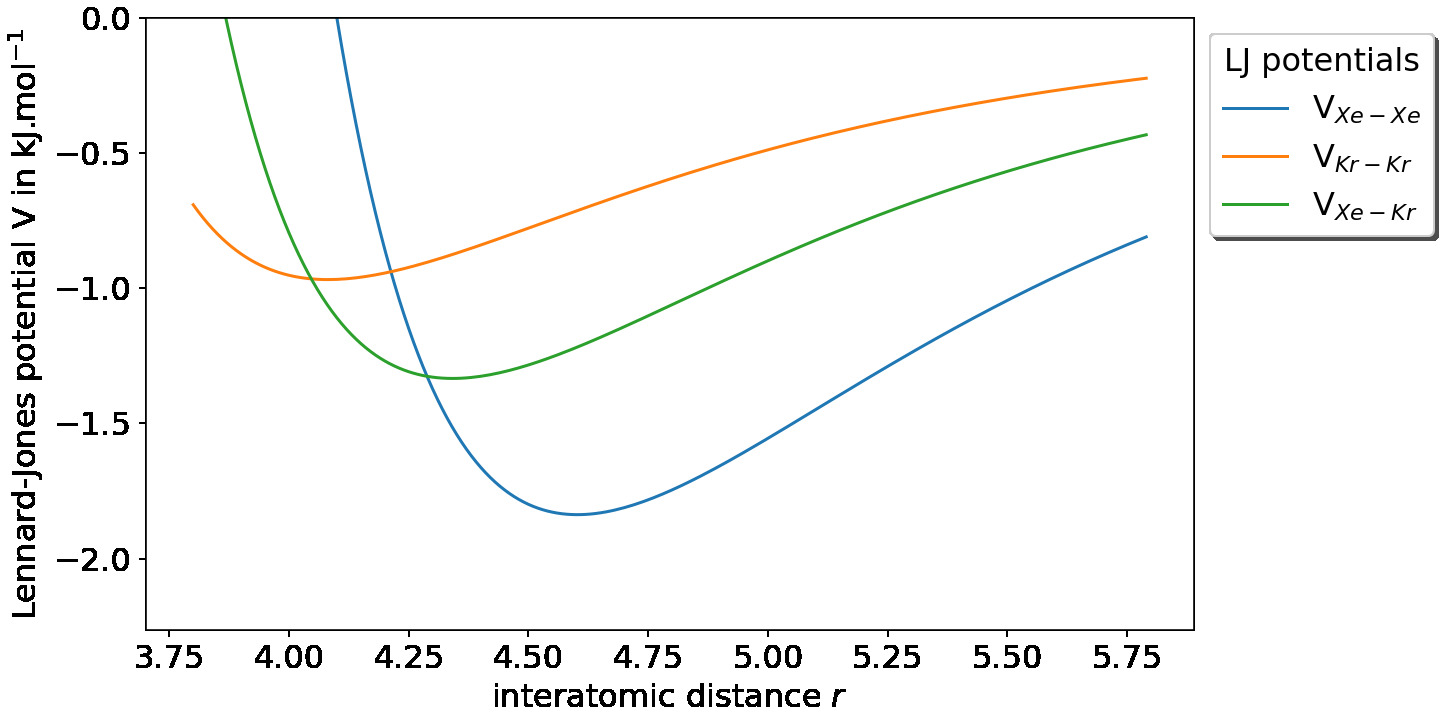
\includegraphics[width=0.6\textwidth]{figures/2-thermo/lennard_jones.jpg}
    \caption{\ The LJ potentials for xenon and krypton interactions. The xenon-xenon interaction is more stabilizing than the krypton-krypton interaction for interatomic distance higher than \SI{4.2}{\angstrom}.}\label{fgr:LJ}
  \end{figure}

In the case of \texttt{KAXQIL}, the material features one-dimensional tubes as channels (Figure~\ref{fgr:SI:examples:KAXQIL}), with a distance between two adsorption sites that is approximately the unit cell parameter along the tube direction (\SI{5.6}{\angstrom}). The selectivity of this material increases with pore filling, primarily driven by enthalpic considerations, which can be explained through a relatively straightforward rationale. By estimating the Lennard-Jones potentials $U\ex{LJ}$ for all species at a distance of \SI{5.6}{\angstrom}: $U\ex{LJ}\e{Xe-Xe}=-1.0$\,\si{\kilo\joule\per\mol}, $U\ex{LJ}\e{Kr-Kr}=-0.3$\,\si{\kilo\joule\per\mol} and $U\ex{LJ}\e{Xe-Kr}=-0.5$\,\si{\kilo\joule\per\mol}. In a simplified model where all adsorbed molecules are assumed to be \SI{5.6}{\angstrom} apart, the cooperative effect between two xenon molecules is more significant, which accounts for the increased selectivity at high uptake. Further analysis of the adsorption enthalpies of xenon and krypton (\emph{cf.} Table~\ref{tbl:thermo}) reveals that both values increase. This can be attributed to the guest molecules deviating from the ``ideal'' adsorption sites, resulting in guest-guest interactions that do not fully compensate. Consequently, the selectivity change observed in this material is a consequence of the rearrangement of adsorbate positions within the nanopores, driven by guest-guest interactions. 

\begin{figure*}[ht]
  \centering
    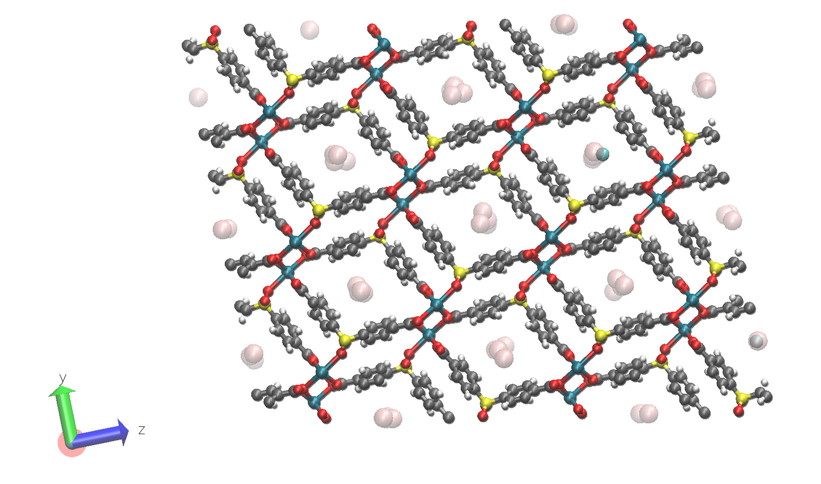
\includegraphics[width=0.45\textwidth]{figures/2-thermo/KAXQIL_clean.jpg}
    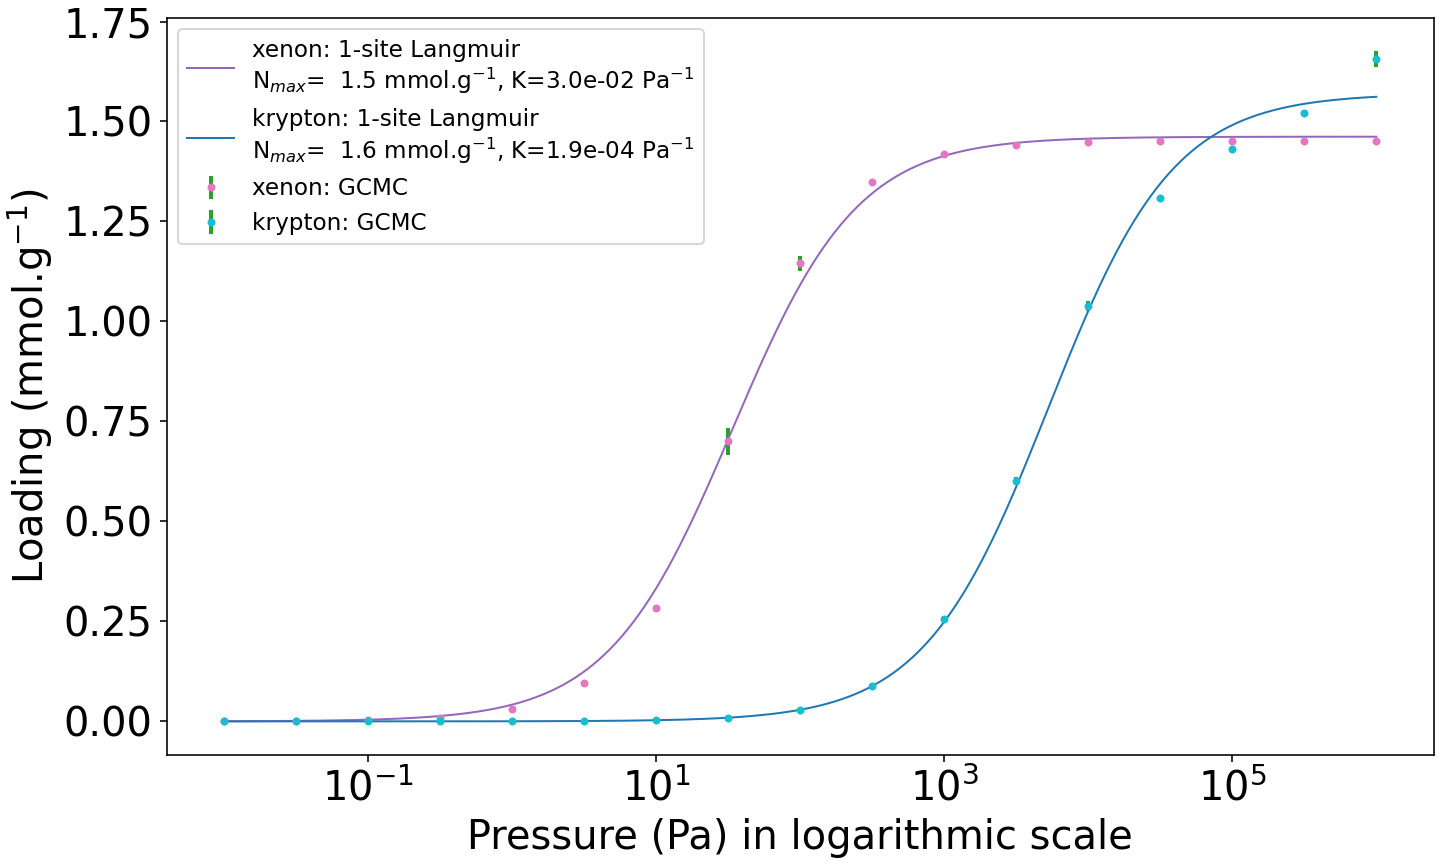
\includegraphics[width=0.45\textwidth]{figures/2-thermo/KAXQIL_clean_isotherm_xenon_krypton_298K.jpg}
    \caption{\texttt{KAXQIL}: On the left side, an illustration of a clean version (all solvent removed) of the calcium coordination framework [Ca(SDB)]$\cdot$H$_2$O, where SDB = 4,$4'$-sulfonyldibenzoate loaded with xenon and krypton obtained by GCMC calculations. Color code: Ca in dark cyan, C in gray, O in red, H in white, S in yellow; Xe in transparent pink and Kr in cyan for the adsorbates. The mono-component isotherms fitted with a 1-site Langmuir model (equation~\ref{eq:langmuir_1}) for both xenon and krypton at \SI{298}{\kelvin} is represented on the right side.}\label{fgr:SI:examples:KAXQIL}
  \end{figure*}

To further validate the role of the guest--guest interactions, another material with one-dimensional tubelike channels is considered: \texttt{JUFBIX}, a cobalt(II) coordination polymer based on carboxylic acid linkers (Figure~\ref{fgr:SI:examples:JUFBIX}).\autocite{JUFBIX} The periodicity along the tube direction is significantly larger at $7.2$\,\si{\angstrom}. The pair interaction energies corresponding to the LJ potentials at this distance are determined as $U\ex{LJ}\e{Xe-Xe}=-0.24$\,\si{\kilo\joule\per\mol}, $U\ex{LJ}\e{Kr-Kr}=-0.06$\,\si{\kilo\joule\per\mol} and $U\ex{LJ}\e{Xe-Kr}=-0.13$\,\si{\kilo\joule\per\mol}. Upon analyzing the adsorption enthalpies (Table~\ref{tbl:effect}), it is observed that these values are too small to affect the positioning of the adsorbed molecules. When the loading is high, resulting in a significant distance between the adsorbed molecules, each adsorption site becomes independent of others. Consequently, the ambient-pressure selectivity $s\e{1}$ remains equal to the low-pressure selectivity $s\e{0}$ since the guest--guest interactions become negligible. This finding substantiates the critical role played by cooperative effects among guest molecules when considering a saturated material.

\begin{figure*}[ht]
  \centering
    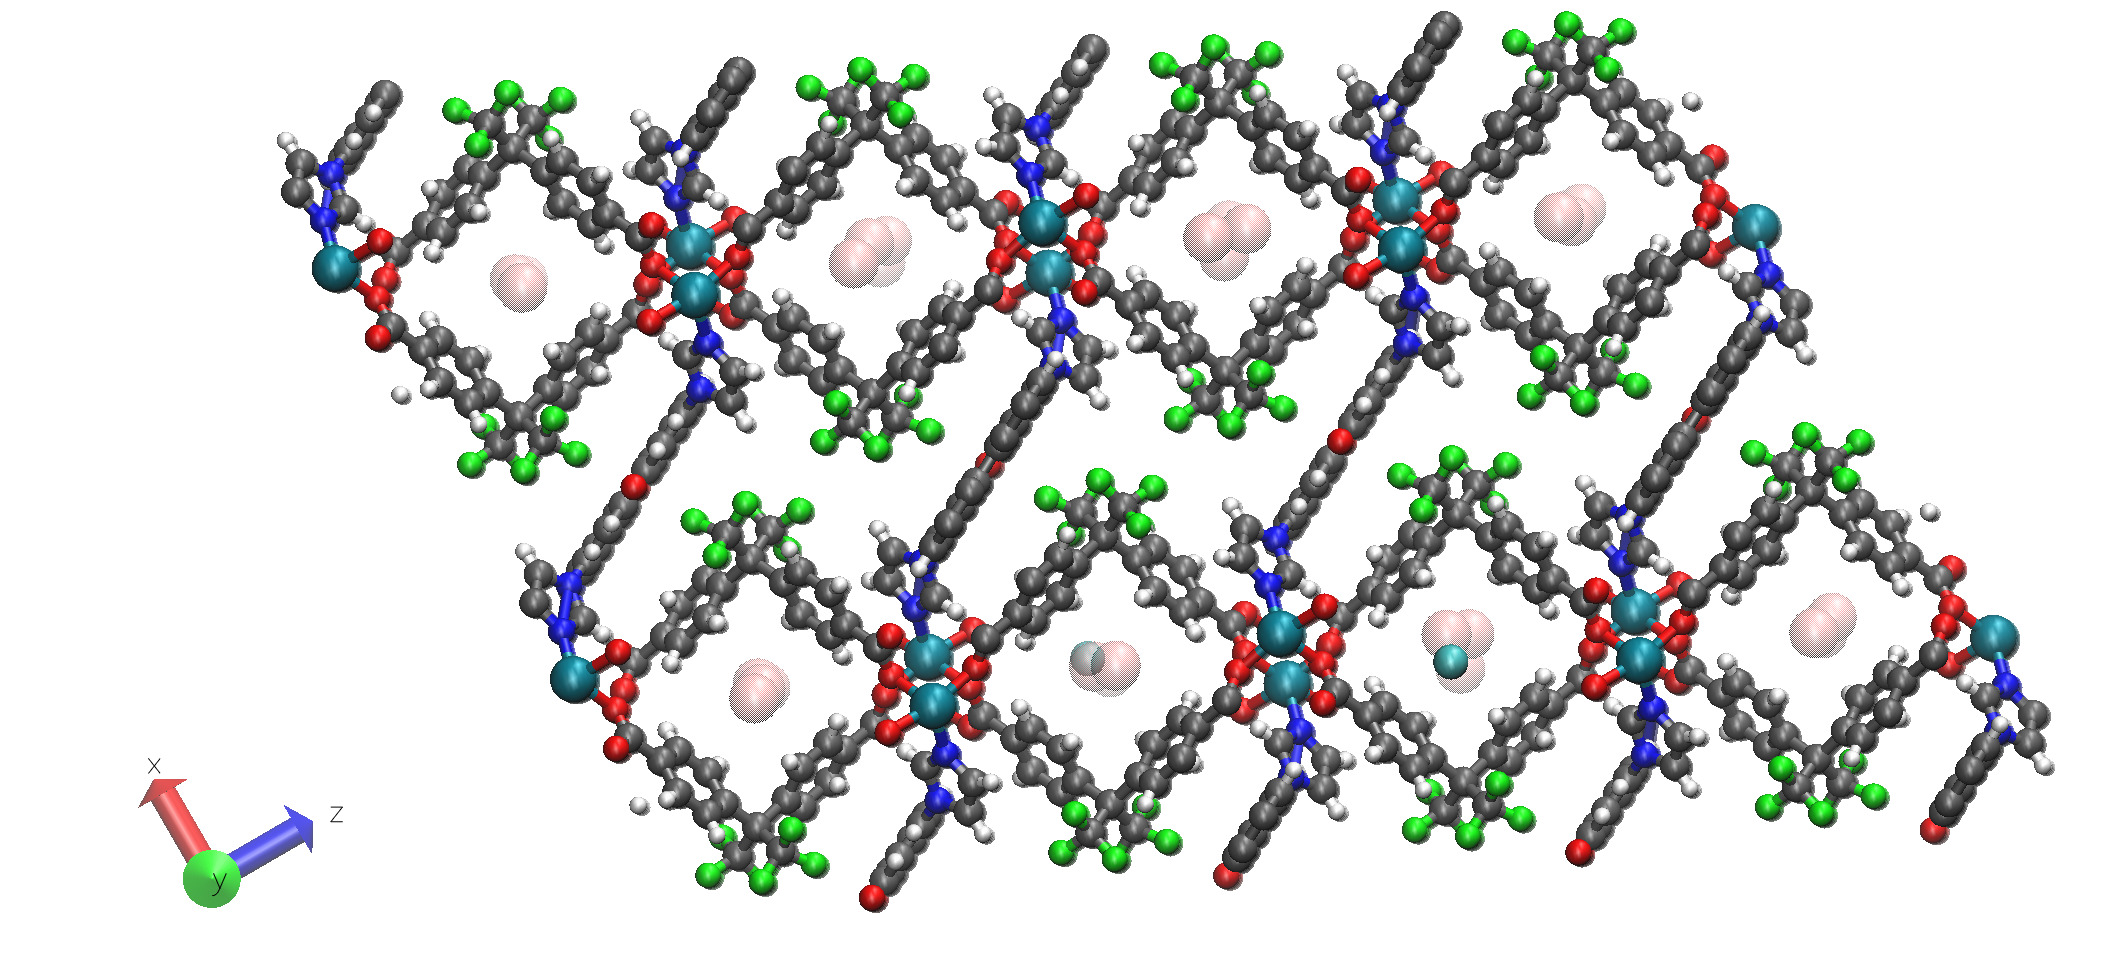
\includegraphics[width=0.45\textwidth]{figures/2-thermo/JUFBIX_clean.jpg}
    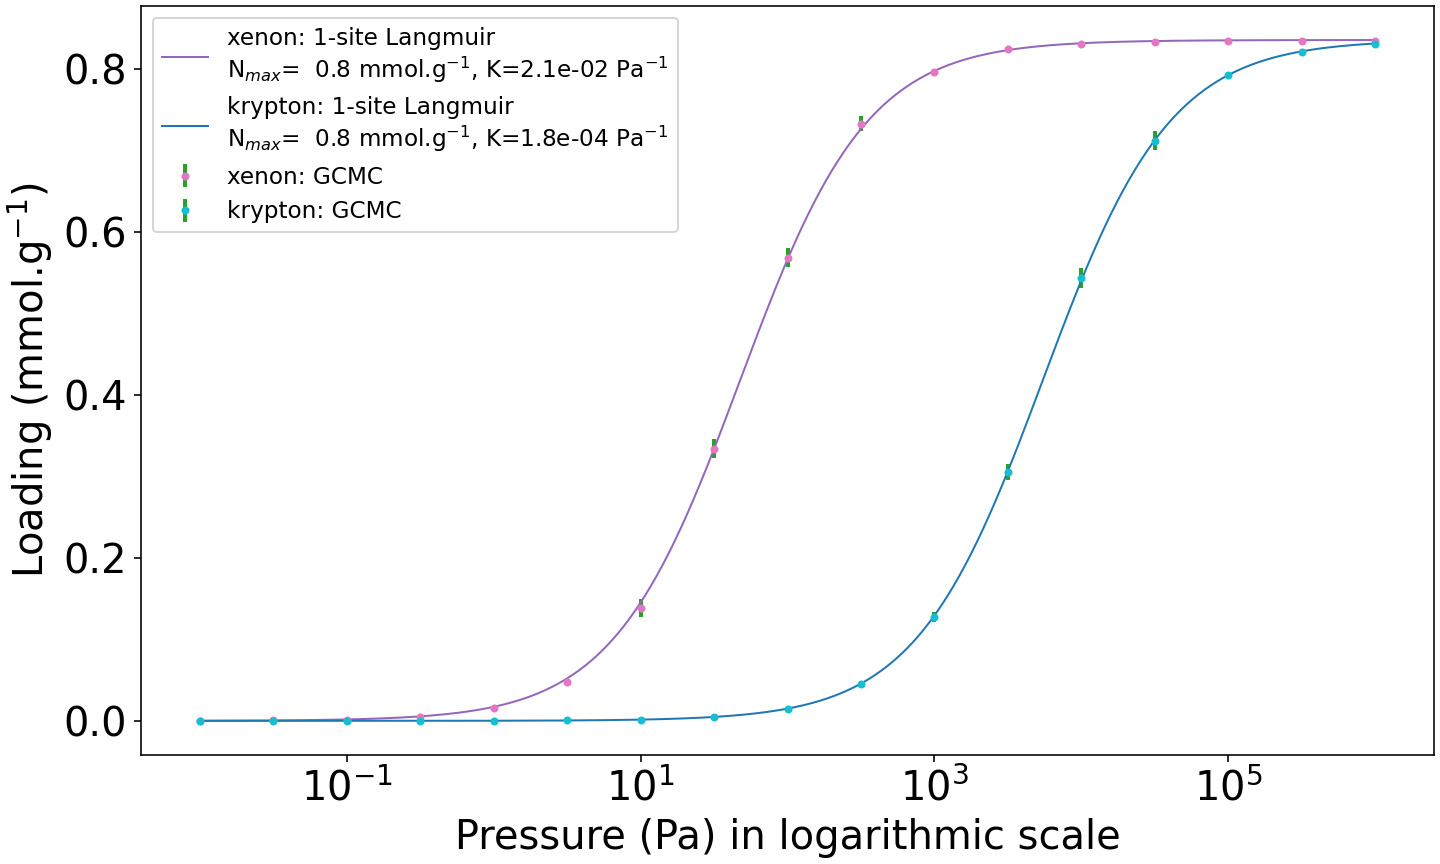
\includegraphics[width=0.45\textwidth]{figures/2-thermo/JUFBIX_clean_isotherm_xenon_krypton_298K.jpg}
    \caption{\texttt{JUFBIX}: Representation of a clean version (all solvent removed) of the cobalt(II) coordination framework [Co$_2$(L)(ppda)$_2$]$_2\cdot$H$_2$O, where the ligand L is 2,8-di(1\emph{H}-imidazol-1-yl)dibenzofuran and the carboxylic acid ligand H$_2$ppda is 4,$4'$-(perfluoropropane-2,2-diyl)dibenzoic acid loaded with xenon and krypton obtained by GCMC calculations. Color code: Co in dark cyan, C in gray, O in red, H in white, N in blue, F in green ; Xe in transparent pink and Kr in cyan for the adsorbates. The mono-component isotherms fitted with a 1-site Langmuir model (equation~\ref{eq:langmuir_1}) for both xenon and krypton at \SI{298}{\kelvin} is represented on the right side.}\label{fgr:SI:examples:JUFBIX}
  \end{figure*}

  \texttt{GOMREG} and \texttt{JAVTAC} are two frameworks categorized as materials with a moderate decrease in selectivity from low to ambient pressure. In the case of GOMREG, the channels consist of one-dimensional tubes that are larger compared to \texttt{KAXQIL} or \texttt{JUFBIX} (Figure~\ref{fgr:SI:examples:GOMREG} and Table~\ref{tbl:effect}). The adsorption sites alternate from left to right inside the channels, resulting in an organized ``zigzag'' pattern of adsorbed molecules. Analyzing the adsorption enthalpies, it is observed that both xenon and krypton exhibit lower enthalpies by a similar margin, indicating an equivalent stabilization for both atoms. Consequently, the enthalpic contribution to the selectivity change is close to 1. 
Due to its smaller size and weaker interaction with the adsorption site, Krypton has more available space within the pore structure. This leads to an entropic advantage for Kr, as reflected by the entropic contribution $k\e{S}$ of $0.64$ in Table~\ref{tbl:effect}. These findings suggest that while enthalpic considerations primarily account for the observed changes at a statistical level, as discussed in previous sections, entropic considerations can play a significant role in pressure-dependent selectivity for specific cases.

\begin{figure*}[ht]
  \centering
    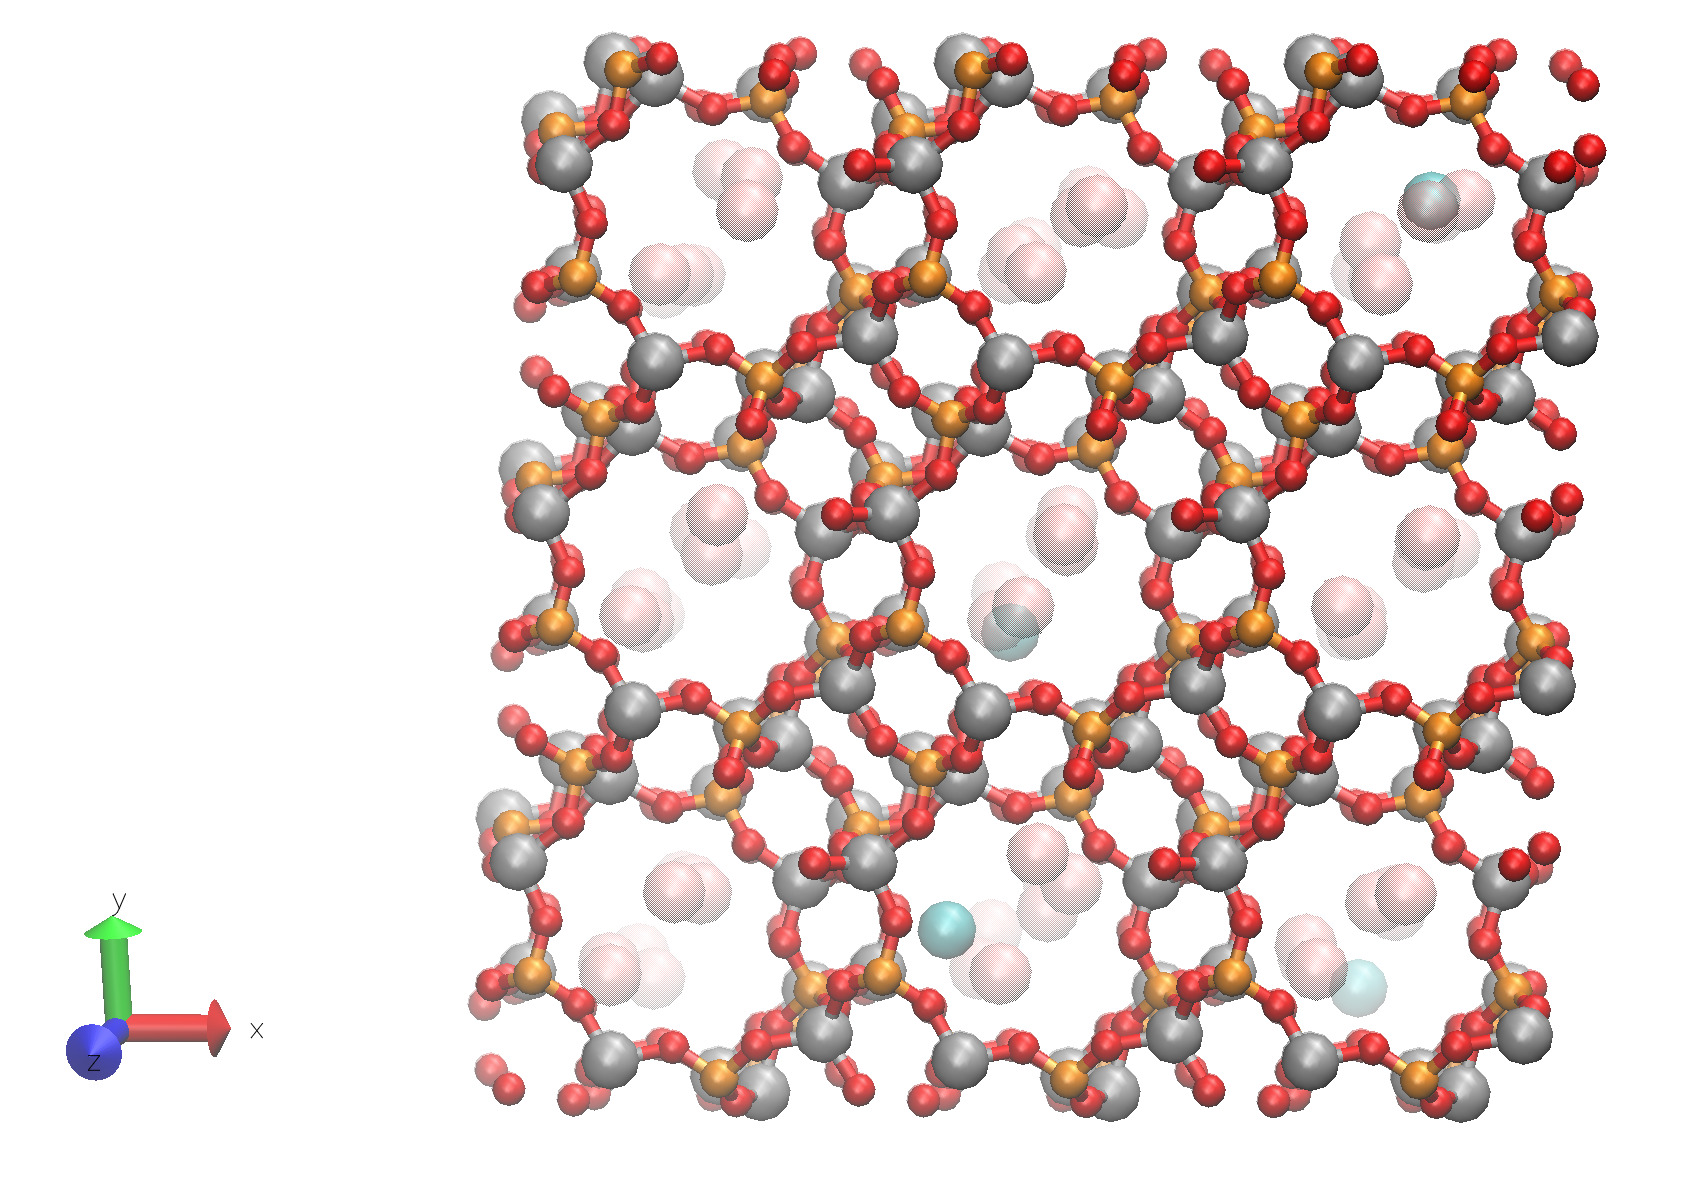
\includegraphics[width=0.45\textwidth]{figures/2-thermo/GOMREG_clean.jpg}
    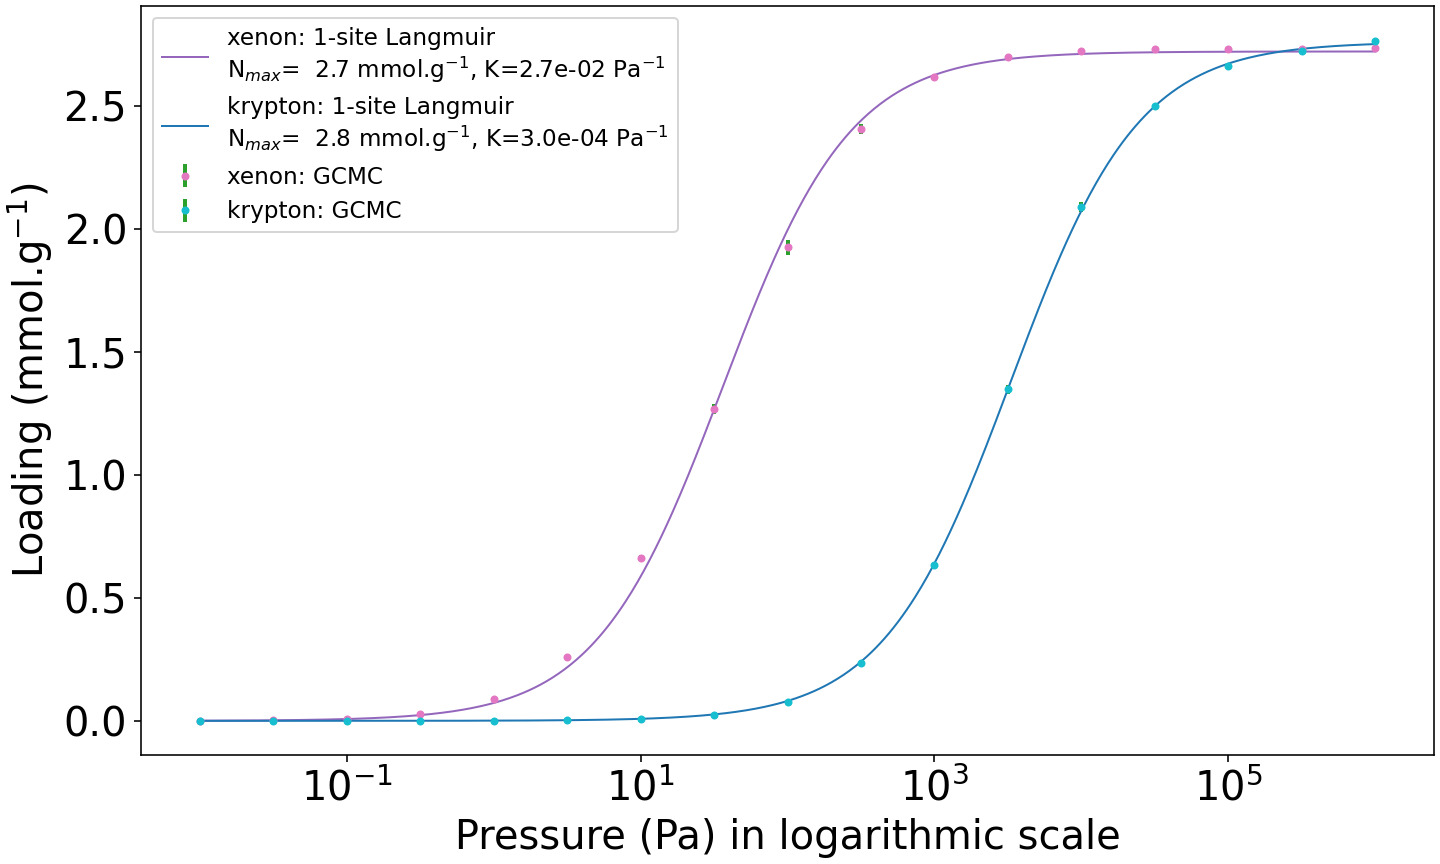
\includegraphics[width=0.45\textwidth]{figures/2-thermo/GOMREG_clean_isotherm_xenon_krypton_298K.jpg}
    \caption{\texttt{GOMREG}: Representation of a clean version (all solvent removed) of this aluminophosphate AlPO$_4$-$n$ that has a zeotype LAU topology with one-dimensional 10-ring channels loaded with xenon and krypton obtained by GCMC calculations. Color code: Al in silver, P in orange, O in red ; Xe in transparent pink and Kr in cyan for the adsorbates. The mono-component isotherms fitted with a 1-site Langmuir model (equation~\ref{eq:langmuir_1}) for both xenon and krypton at \SI{298}{\kelvin} is represented on the right side.}\label{fgr:SI:examples:GOMREG}
  \end{figure*}

The remaining materials discussed in this third category exhibit a significant decrease in selectivity from low to ambient pressure. To investigate the factors contributing to this decrease, several phenomena that are relevant for screening studies have been examined, as they can impose limitations on the working performance of materials that initially appear to be ``top performer'' based on zero-pressure screening.


For example, \texttt{GOMRAC} has a similar structure compared to \texttt{GOMREG} (Figure~\ref{fgr:SI:examples:GOMRAC}), with the distinction of having smaller pores and channels are smaller (see the values of the D$_i$, and the D$_f$, in Table~\ref{tbl:effect}). Consequently, the distances between adsorbed molecules--- in their ideal sites ---  are smaller. At such close distances, it is reasonable to assume that the interactions between adsorbates favor krypton over xenon molecules in GOMRAC (see LJ potentials at distance lower than \SI{4.2}{\angstrom} in Figure~\ref{fgr:LJ}). This enhanced stabilization of krypton relative to xenon results in an enthalpic contribution $k\e{H}$ of $0.58$. Moreover, this finding is consistent with the equivalent guest--guest interactions observed in \texttt{GOMREG}, as discussed earlier. It explains why the difference in adsorption enthalpies becomes smaller for \texttt{GOMRAC}, while it remains unchanged for \texttt{GOMREG} (between low and ambient pressure). This further validates the critical role of interactions between adsorbed molecules and their dependence on guest-guest distances, particularly under high loading conditions.

\begin{figure*}[ht]
  \centering
    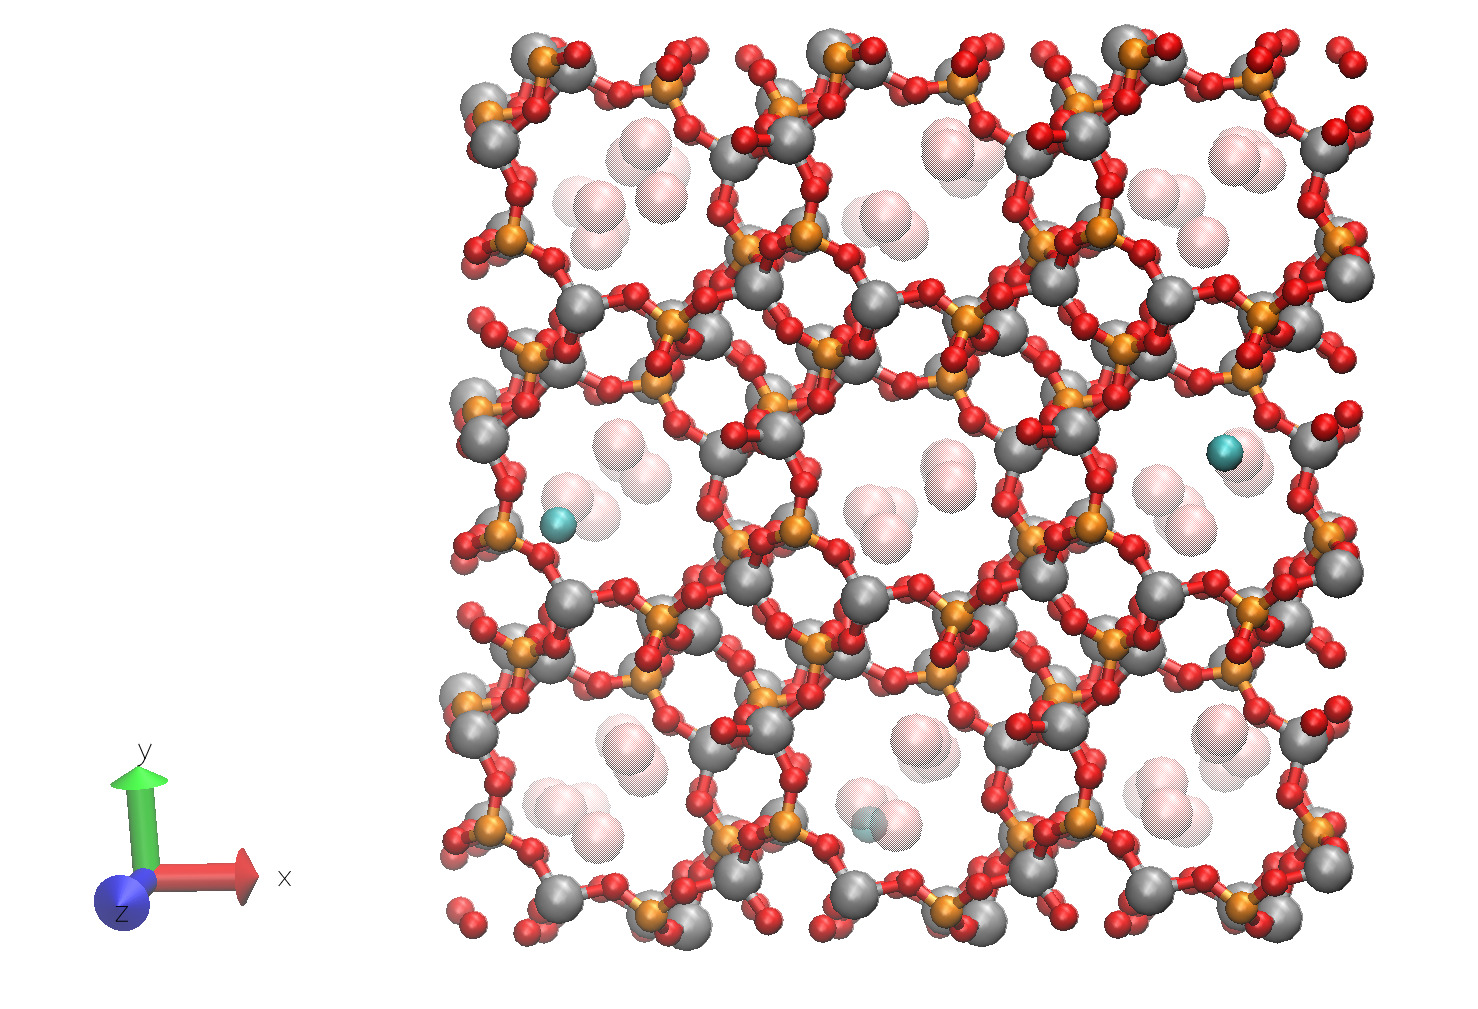
\includegraphics[width=0.45\textwidth]{figures/2-thermo/GOMRAC_clean.jpg}
    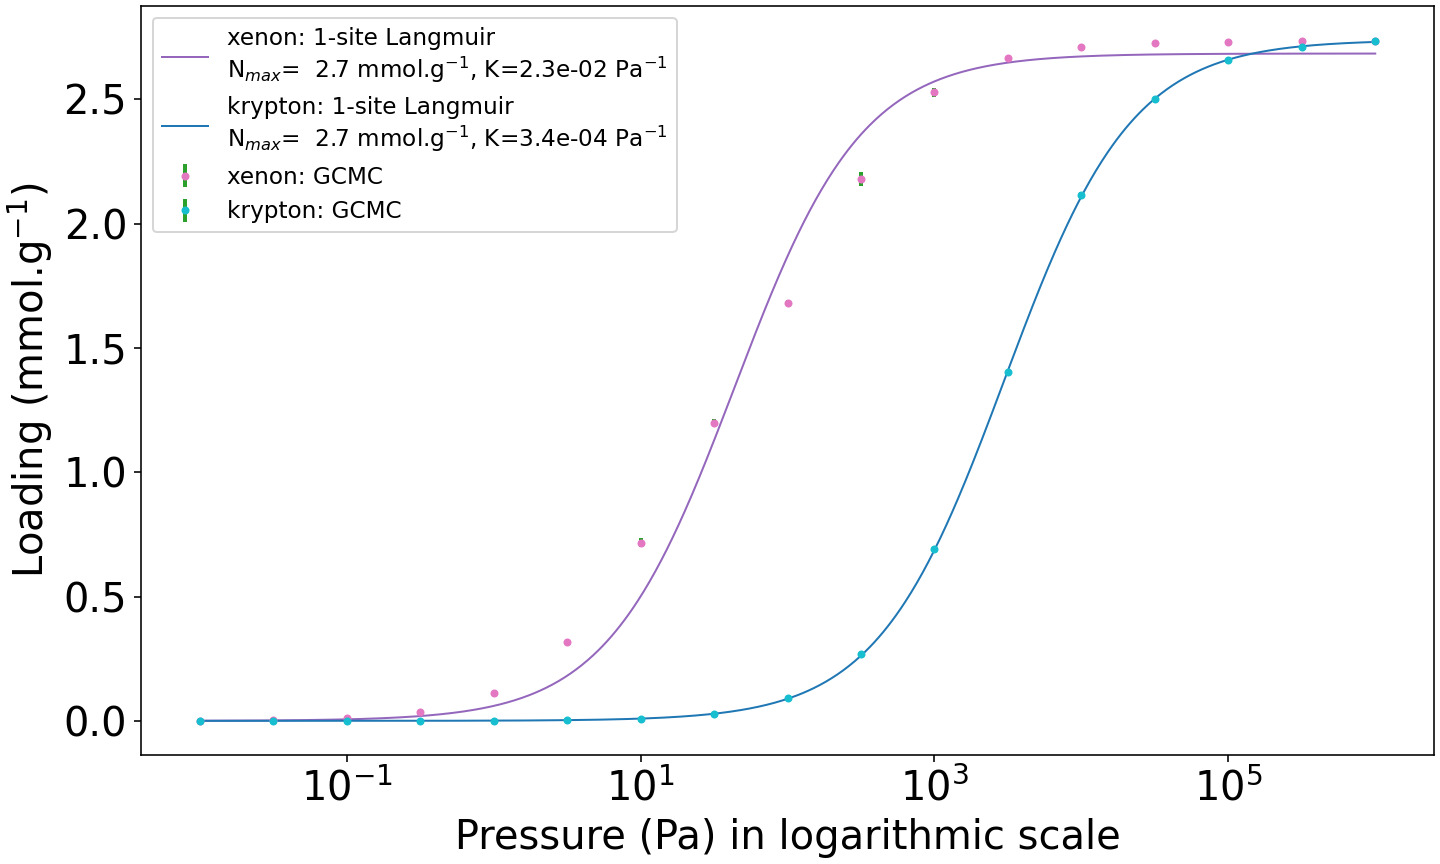
\includegraphics[width=0.45\textwidth]{figures/2-thermo/GOMRAC_clean_isotherm_xenon_krypton_298K.jpg}
    \caption{\texttt{GOMRAC}: Representation of a clean version (all solvent removed) of this aluminophosphate AlPO$_4$-$n$ that has a zeotype LAU topology with one-dimensional 10-ring channels loaded with xenon and krypton obtained by GCMC calculations. Color code: Al in silver, P in orange, O in red; Xe in transparent pink and Kr in cyan for the adsorbates. The mono-component isotherms fitted with a 1-site Langmuir model (equation~\ref{eq:langmuir_1}) for both xenon and krypton at \SI{298}{\kelvin} is represented on the right side. It seems that this aluminophosphate is just a smaller version of \texttt{GOMREG}.}\label{fgr:SI:examples:GOMRAC}
  \end{figure*}

In the case of \texttt{MISQIQ}, the pure-component Xe isotherm depicted in Figure~\ref{fgr:MISQIQ} oes not conform to a single-site Langmuir isotherm, but rather aligns well with a two-site Langmuir model (Figure~\ref{fgr:MISQIQ}). Upon visual examination of the adsorbed density at various loadings, it becomes evident that the second step in the isotherm (representing about {20\%} of the uptake at full loading) corresponds to a reorganization of the adsorbate molecules accompanied by a contraction of interatomic distances. It is important to note that this reorganization does not involve the occupation of a distinct and separate adsorption site at high loading. In this case, the change in selectivity can be attributed to the potential for adsorbate reorganization within the nanopores of the material. This reorganization, which can be detected through the xenon isotherm alone, plays a significant role in determining the material's selectivity at ambient pressure. The repacking of the adsorbed phase during this reorganization process is associated with a strong entropic effect and also influences the enthalpic contribution to selectivity.

\begin{figure*}[t]
  \centering
    \includegraphics[width=0.48\textwidth]{figures/2-thermo/MISQIQ_clean.jpg}\hfill
    \includegraphics[width=0.48\textwidth]{figures/2-thermo/MISQIQ_clean_isotherm_xenon_krypton_298K.jpg}
    \caption{Representation of a chiral open-framework fluoroaluminophosphate [C$_4$N$_3$H$_{16}$]$\cdot$[Al$_6$P$_3$O$_{12}$F$_6$(OH)$_6$] denoted AlPO-JU89 (referenced \texttt{MISQIQ} in the Cambridge structural database), which has been loaded with xenon and krypton in a GCMC simulation, on the left side.\autocite{MISQIQ} Color code: Al in silver, P in orange, O in red, H in white and F in green for the framework; Xe in transparent pink and Kr in cyan for the adsorbates. The pure-component isotherms fitted with a 2-site Langmuir model (equation~\ref{eq:langmuir_2}) for both xenon and krypton at \SI{298}{\kelvin} on the right side.}\label{fgr:MISQIQ}
  \end{figure*}

The materials \texttt{BAEDTA01}, \texttt{VIWMOF}, \texttt{LUDLAZ}, \texttt{WOJJOV}, and \texttt{VAPBIZ} fall into the category of having more than one available adsorption site, resulting in a significant drop in selectivity from low to ambient pressure. The pure-component isotherms and the representation of the materials loaded in xenon and krypton molecules (presented in the supporting information of the Ref.~\cite{Ren_2021} Figures~S19-23) confirm the existence of at least two distinct adsorption sites in each material. The preferential filling of the most selective sites (i.e., the most favorable for Xe) occurs at low loading, while the less selective sites are populated as the pressure increases. Consequently, a net decrease in selectivity at ambient pressure is observed for these materials. The existence of different types of adsorption sites and their impact on Xe/Kr selectivity (at non-zero pressure) suggests the inclusion of this factor in the screening of pure-component isotherms without the need for explicit multi-component GCMC simulations.

\section{Towards the development of new screening tools}

In the current state of the art on Xe/Kr separation by adsorption in nanoporous materials, many studies have focused on establishing structure/property relationships, determining theoretical performance limits, and identifying top-performing materials, for both existing experimental structures and novel hypothetical structures yet to be synthesized. To provide a better understanding of the thermodynamics underlying Xe/Kr separation and the microscopic origins of selectivity at low and ambient pressure, a high-throughput screening of Xe, Kr was conducted as well as Xe/Kr mixtures in 12\,020 experimental open-framework materials. In addition to structural descriptors such as pore sizes, volume, and surface area, thermodynamic quantities were considered to gain insights into the key factors yielding a high selectivity.

The statistical correlation found between Henry's constant for Xe and Xe/Kr selectivity showed that the most selective materials are those with the highest affinity for xenon. To some degree of accuracy, it can be concluded that a direct screening of Kr or xenon adsorption free energy may not be essential for a coarse-grained evaluation of the selectivity of nanoporous frameworks. This finding could facilitate the development of more efficient screening methodologies. For instance, a multistage approach could be employed, starting with a preliminary selection on Henry's constant, which is computationally inexpensive. Subsequently, more computationally intensive grand canonical Monte Carlo (GCMC) simulations can be performed on the selected materials (a gain that can be between 5 and 10-fold in our setup). Furthermore, inspection of the correlations between enthalpy and entropy contributions at low pressure showed that the adsorption-based separation process in the open frameworks studied is mainly enthalpic in nature. It is possible to extend the study in the future to other classes of nanoporous materials beyond MOFs, including covalent organic frameworks, porous aromatic frameworks, purely inorganic porous frameworks such as zeolites, but also amorphous porous materials such as porous polymer membranes.

In the context of xenon-krypton separation using nanoporous materials, pressure swing adsorption (PSA) processes have been widely used, making pressure a crucial thermodynamic variable in the separation cycle. This study has focused on the selectivity difference between a system under very low pressure (at the zero loading limit, which is calculated at relatively low computational cost) and ambient pressure (closer to working conditions but requiring higher simulation cost). The results demonstrated that selectivity can be highly dependent on pressure, with certain materials maintaining high selectivity at both low and ambient pressures, while others experience a significant drop in selectivity. It was found that high ambient-pressure selectivity requires high low-pressure selectivity, but the reverse is not necessarily true.

By using a thermodynamic approach to describe the separation selectivity, the differences in selectivity were elucidated between different pressures (and therefore different loading regimes of the frameworks), primarily attributed to the variations in adsorption enthalpies for Xe and Kr.By delving into specific examples, the microscopic origins of these selectivity changes were uncovered and linked to the relative contributions of host--guest and guest--guest interactions. The population of different adsorption sites or repacking of the adsorbed phase at higher loadings can lead to significant alterations in overall selectivity. The underlying mechanisms of selectivity at high pressure are complex and unique to each framework, requiring a good understanding of the interactions between guest molecules constrained in the nanopores. Nevertheless, this proposed classification of the interactions at play can guide the future design of more efficient high-throughput screening procedures.

For instance, the essentially enthalpic nature of the xenon/krypton separation process underscores the importance of developing more efficient methods for sampling interaction energies and utilizing them as cost-effective descriptors for analyzing an increasing number of structures. In the subsequent chapter, different approaches for evaluating adsorption enthalpy will be explored, considering the computation time required and the accuracy of each method. Additionally, the influence of partial pressure, manifested through changes in composition or pressure, raises questions about the potential use of infinite dilution thermodynamic quantities to predict selectivity at any pressure (GCMC). Numerous studies have focused on predicting GCMC simulations.\autocite{Simon_2015,Shi_2023,Kang_2023,Li_2023}. The thermodynamics-based approach combined with characterizing pore diversity holds the potential to yield improved results in predicting GCMC values of selectivity, contributing to a more comprehensive understanding of adsorption processes in nanoporous materials.


\OnlyInSubfile{\printglobalbibliography}

\end{document}
